%%%%%%%%%%%%%%%%%%%%%%%%%%%%%%%%%%%%%%%%%%%%%%%%%%%%%%%%%%%%%%%%%%%%%%%%%%%%%%%%
%%%%%%%%%%%%%%%%%%   Vorlage für eine Abschlussarbeit   %%%%%%%%%%%%%%%%%%%%%%%%
%%%%%%%%%%%%%%%%%%%%%%%%%%%%%%%%%%%%%%%%%%%%%%%%%%%%%%%%%%%%%%%%%%%%%%%%%%%%%%%%

% Erstellt von Maximilian Nöthe, <maximilian.noethe@tu-dortmund.de>
% ausgelegt für lualatex und Biblatex mit biber

% Kompilieren mit 
% lualatex dateiname.tex
% biber dateiname.bcf
% lualatex dateiname.tex
% lualatex dateiname.tex


% Präambel einbinden:

%------------------------------------------------------------------------------
%---------------- Docmentenklasse, Layout und Ränder: -------------------------
%------------------------------------------------------------------------------
\RequirePackage{fixltx2e}
\documentclass[
        paper=a4,               % Papierformat DIN A4
        BCOR=12mm,              % 12mm Binderandkorrektur
        %parskip=false,           % Absätze als halbe Leerzeile
        headsepline,            % Linie zwischen Kopfzeile und Dokument
        cleardoublepage=plain,  % Keine Kopf/Fußzeile auf Leerseiten
        bibliography=totoc,     % Bibliographie als nicht-nummeriertes 
                                % Kapitel im Inhaltsverzeichnis
        open=right,             % Kapitel beginnen immer aufrechten Seiten
        open=any,               % Kapitel dürfen auf beiden Seiten beginnen
        numbers=noenddot,       % Keine Punkte nach Abbildungsnummern
        captions=tableheading,  % Spacing für Captions über Tabellen an
        titlepage=firstiscover, % Titelseite ist Deckblatt, symmetrische Ränder
        %headings=normal         % kleinere Überschriften
    ]
    {scrbook}


% Patch für LaTeX laden:

% Warnung, falls erneut kompilirt werden muss:
\usepackage[aux]{rerunfilecheck}

% Beschränkung auf chapter und section im Inhaltsverzeichnis:            
\setcounter{tocdepth}{1}

%------------------------------------------------------------------------------
%------------------------------ Sprache und Schrift: --------------------------
%------------------------------------------------------------------------------

% Deutsche Spracheinstellungen
\usepackage{polyglossia}
\setdefaultlanguage{german}

% stellt den \enquote{} Befehl
\usepackage[autostyle]{csquotes}

% verbessert das allgemeine Schriftbild:
\usepackage{microtype}

\usepackage{fontspec}
\defaultfontfeatures{Ligatures=TeX}


\hyphenation{Si-mu-la-tions-ket-te}


%------------------------------------------------------------------------------
%-------------------------   Kopf/Fußzeile/Farben------------------------------
%------------------------------------------------------------------------------


\usepackage{xcolor}
\xdefinecolor{tugreen}{RGB}{128, 186, 38}

\usepackage{scrlayer-scrpage}
\pagestyle{scrheadings}

\addtokomafont{title}{\color{tugreen}}          % Titel auf der Titelseite in TU-Grün
\addtokomafont{sectioning}{\color{tugreen}}     % Kapitel-Überschriften in TU-Grün
\addtokomafont{pagenumber}{\color{tugreen}}     % Seitenzahl in TU-Grün
\addtokomafont{chapterentry}{\color{tugreen}}   % Inhaltsverziechnis
\setheadsepline{0.75pt}[\color{tugreen}]        % Linie unter Kopzzeile in TU-Grün


%------------------------------------------------------------------------------
%------------------------ Für die Matheumgebung--------------------------------
%------------------------------------------------------------------------------

\usepackage{amsmath}
\usepackage{amssymb}
\usepackage{mathtools}

% Enable Unicode-Math and follow the ISO-Standards for typesetting math
\usepackage[
  math-style=ISO,
  bold-style=ISO,
  sans-style=italic,
  nabla=upright,
  partial=upright,
]{unicode-math}
\setmathfont{Latin Modern Math}

% schöne Brüche im Text mit \sfrac{}{}
\usepackage{xfrac}  


%Gleichungsnummern Kapitel.Unterkapitel.Gleichung
\renewcommand{\theequation}{\thechapter{}.\arabic{equation}}
\numberwithin{equation}{chapter}


%------------------------------------------------------------------------------
%---------------------------- Einheiten ---------------------------------------
%------------------------------------------------------------------------------

\usepackage[
  locale=DE,
  separate-uncertainty=true,
  per-mode=symbol-or-fraction,
]{siunitx}
\sisetup{math-micro=\text{µ},text-micro=µ}

%------------------------------------------------------------------------------
%------------------------------ Tabellen: -------------------------------------
%------------------------------------------------------------------------------

\usepackage{booktabs}       % stellt \toprule, \midrule, \bottomrule
\usepackage{threeparttable} % für komplexere Tabellen

%------------------------------------------------------------------------------
%------------------------------ Grafiken: -------------------------------------
%------------------------------------------------------------------------------

\usepackage[]{graphicx}

\usepackage{grffile}

\usepackage{scrhack}
\usepackage{float}
\floatplacement{figure}{htbp}
\floatplacement{table}{htbp}
\usepackage[section]{placeins}

\usepackage{caption}
\DeclareCaptionFont{tugreen}{\color{tugreen}}
\captionsetup{%
            labelfont={bf,tugreen},     % Label fett und in TU-Grün
            format=plain,               % Caption-Text steht auch unter "Tabelle x"
            width=0.9\textwidth         % Bereich für Caption schmaler als für Text
           }

\usepackage{subcaption}   % for subfigures


%------------------------------------------------------------------------------
%------------------------------ Bibliographie ---------------------------------
%------------------------------------------------------------------------------

\usepackage[backend=biber]{biblatex}    % Biblatex mit biber
    \addbibresource{references.bib}     % die Bibliographie einbinden

\DefineBibliographyStrings{ngerman}{andothers = {{et\,al\adddot}}}


%------------------------------------------------------------------------------
%------------------------------ Sonstiges: ------------------------------------
%------------------------------------------------------------------------------


\usepackage{eurosym}
\usepackage[pdfusetitle,unicode, linkbordercolor=tugreen]{hyperref}
\usepackage{bookmark}
\usepackage[shortcuts]{extdash}
\usepackage{todonotes}





%------------------------------------------------------------------------------
%-------------------------    Angaben zur Arbeit   ----------------------------
%------------------------------------------------------------------------------

%Titel der Arbeit
%\newcommand{\thetitle}{Analyse der Quelle Markarian 421\\ während des MAGIC-Upgrades 2012}
%\newcommand{\thesubtitle}{oder\\ Die Rolle der Monte Carlo-Produktion in der MAGIC-Datenanalyse}

\newcommand{\thetitle}{Von der Monte-Carlo-Produktion zur Datenanalyse}
\newcommand{\thesubtitle}{-\\ Eine Analyse der 2012 genommenen Daten \\ des Aktiven Galaktischen Kerns Mrk 421}


\newcommand{\Geburtsort}{Willich}
\newcommand{\Jahr}{Mai 2015}
\newcommand{\Lehrstuhl}{Experimentelle Physik V}
\newcommand{\Betreuer}{Prof. Dr. Erstgutachter}
\newcommand{\Zweitgutachter}{Prof. Dr. Zweitgutachter}
\newcommand{\Abgabedatum}{11. Juli 2014}

%Author und Email-Adresse
\author{
   \textbf{Katharina Frantzen}\\
   geboren in \Geburtsort
}

\titlehead{
   
\includegraphics[height=1.5cm]{logos/tu-logo.pdf}
}
\title{\thetitle}
\subtitle{\thesubtitle}

\date{\Jahr}

\subject{Arbeit zur Erlangung des akademischen Grades eines \\Doktors der Naturwissenschaften \\(Dr. rer. nat.)}
\publishers{Lehrstuhl für \Lehrstuhl \\ Fakultät Physik \\ Technische Universität Dortmund}


\begin{document}
\frontmatter
\maketitle
%Gutachterseite
\thispagestyle{empty}
\vspace*{\fill}
\begin{tabbing}
   Erstgutachter: \hspace{3em}\=   \Betreuer \\ 
   Zweitgutachter: \> \Zweitgutachter\\
   Abgabedatum: \>\Abgabedatum
\end{tabbing}
\newpage

% hier beginnt der Vorspann, nummeriert in römischen Zahlen
%\thispagestyle{plain}
\section*{Kurzfassung}

\textbf{\large Empfohlen wird die Verwendung dieser Vorlage mit der jeweils aktuellsten TeXLive Version (Linux, Windows) bzw. MacTeX Version (MacOS).
Aktuell ist dies TeXLive 2014. Download hier: 
}

\href{https://www.tug.org/texlive/}{\textbf{\large https://www.tug.org/texlive/}}

\textbf{\large
Wichtig ist auch, dass die Source-Dateien UTF-8 kodiert sind. Dies
ist nur unter Windows ein Problem, benutzen Sie einen Editor, der
UTF-8 unterstützt (z.B. TexMaker ab V4, notepad++, sublime).
}

Eine aktuelle Version dieser Vorlage gibt es unter 

\href{https://github.com/MaxNoe/VorlageBachelorArbeit/tree/tu-farben}{www.github.com/MaxNoe/VorlageBachelorArbeit/tree/tu-farben}.

Eine farblich neutrale Variante steht unter  

\href{https://github.com/MaxNoe/VorlageBachelorArbeit}{www.github.com/MaxNoe/VorlageBachelorArbeit}

zur Verfügung.

Falls es Probleme mit der Vorlage gibt, einfach ein \emph{Issue} auf GitHub aufmachen oder eine Email an
\href{mailto:maximilian.noethe@tu-dortmund.de}{maximilian.noethe@tu-dortmund.de} schreiben.


Hier steht eine Kurzfassung der Arbeit in deutscher Sprache inklusive der Zusammenfassung der
Ergebnisse.
Zusammen mit der englischen Zusammenfassung muss sie auf diese Seite passen.

\section*{Abstract}

The abstract is a short summary of the thesis in English, together with the German summary it has to fit on this page.

\tableofcontents

\mainmatter
% Hier beginnt der Inhalt mit Seite 1 in arabischen Ziffern
\chapter{Einleitung}

\begin{quotation}
 Terry Pratchett, einer der berühmtesten Fantasy-Autoren, sagte: 
 
 \enquote{Das Universum ist ein großer Witz}.
 
 %Da denkt man sich: \enquote{\textit{Na, das wollen wir ja mal sehen}.}
 \textit{Ich bin mir da aber noch nicht so sicher...}
\end{quotation}


Vielleicht hilft diese Doktorarbeit dabei, ein kleines bisschen Licht ins Dunkel des Universums zu bringen.
Mit Hilfe von Teilchen, die wir auf der Erde oder mit Hilfe von Satelliten detektieren, können wir versuchen, so viel wie möglich über das Universum zu erfahren.
Fragen wie \enquote{Woher kommen die Teilchen, die wir hier messen?}, \enquote{Wie wurden diese Teilchen beschleunigt?} oder \enquote{Was passiert auf dem Weg von der Quelle bis zu uns mit diesen Teilchen?} beschäftigen die Astroteilchenphysiker.
Um diese Fragen zu klären, stehen verschiedene Botenteilchen mit ihren Vor- und Nachteilen zur Verfügung.
Im Folgenden werde ich mich auf die Gammastrahlung als Bote konzentrieren.\\

Das Konzept der Gammaastronomie wurde in den 50er Jahren entwickelt und in den folgenden Jahren begann die Entwicklung der passenden Teilchendetektoren bis hin zu den abbildenden Luftschauer-Cherenkovdetektoren wie den MAGIC-Teleskopen.
Mit Hilfe dieser beiden Teleskope, die sich auf La Palma befinden, ist es möglich Luftschauer, ausgelöst von sehr hochenergetischer Gammastrahlung, zu detektieren.

Eine mögliche Quelle für hochenergetische Gammastrahlung sind Aktive Galaktische Kerne (AGN).
Die Quellen Markarian~421 (Mrk~421) und Markarian~501 (Mrk~501) waren die ersten detektierten Quellen dieses Typs.
Mrk~421 besitzt eine Rotverschiebung von $z=0.031$ und wurde als Gammastrahlung-emittierende Quelle in den 90er Jahren vom Whipple-Teleskop entdeckt.

Um die physikalischen Prozesse in diesen Quellen zu verstehen, werden Modelle für die Teilchenproduktion und -beschleunigung benötigt.
Die Analyse einer solchen AGN hat unter anderem zum Ziel, das Energiespektrum der emittierten Strahlung zu bestimmen oder eine Lichtkurve anzufertigen, welche die zeitliche Entwicklung des Flusses darstellt.
Dabei gibt es einige Herausforderungen:
Da das Verhältnis von Signal (Gammastrahlung aus der Quelle) zu Untergrund (hadronische Schauer) im besten Fall ca. 1:1000 beträgt, werden effiziente Algorithmen zur Signal-Untergrund-Trennung benötigt.
Diese Klassifikationsalgorithmen werden mit Hilfe von Monte-Carlo-Simulationen trainiert.
Eine genaue Simulation der Primärteilchen, die einen Teilchenschauer auslösen und vom Experiment detektiert werden, ist wichtig.
Alle Simulationsschritte von der Schauersimulation, über die Simulation der Reflexion der Photonen am Teleskopspiegel bis zur Simulation der Kamera und der Elektronik müssen möglichst genau durchgeführt werden.
Dies erfordert die stetige Anpassung der Simulation an die aktuellen Gegebenheiten.
Veränderungen der abbildenden Eigenschaften der Spiegel, sowie Veränderungen in der Elektronik müssen in der Simulation berücksichtigt werden.
Dies führt dazu, dass bei Veränderungen an der Hardware des Teleskops eine neue Monte-Carlo-Produktion angefertigt werden muss.
Die gesamte Monte-Carlo-Produktion für das MAGIC-Experiment wurde im Laufe dieser Doktorarbeit in Dortmund durchgeführt.

Mit Hilfe der Monte-Carlo-Simulationsdaten wird die Analyse der AGN Mrk~421 durchgeführt.
Die zeitliche Entwicklung des Flusses sowie das Energiespektrum dieser Quelle sind die Analyseergebnisse.
Zudem bietet sich die Möglichkeit, eine Quelle in unterschiedlichen Wellenlängen simultan zu observieren.
Diese Multiwellenlängendaten von verschiedenen Experimenten beleuchten die Quelle jeweils in einem anderen Licht und können dabei helfen, physikalische Prozesse wie Beschleunigungsmechanismen und die Produktion von Gammastrahlung zu untersuchen.
Es existieren zwei grundsätzlich unterschiedliche Modelle für die Produktion von Gammastrahlung in diesem Quelltyp, von denen bisher noch keines bestätigt oder ausgeschlossen werden konnte.\newline

Die Arbeit gliedert sich folgendermaßen:

\textbf{\autoref{chapter:Astroteilchenphysik}} gibt einen Einblick in die Astroteilchenphysik. 
Verschiedene Quellen kosmischer Strahlung und Beschleunigungsmechanismen werden vorgestellt. 
Des Weiteren wird auf die Gammaastronomie als eigenes Forschungsgebiet in der Astroteilchenphysik eingegangen. 
Danach wird der Quelltyp des Aktiven Galaktischen Kerns (AGN) näher beschrieben und die in dieser Arbeit analysierte AGN Mrk~421 vorgestellt.

\textbf{\autoref{chapter:MC-Simulation}} beinhaltet eine Beschreibung der MAGIC-Teleskope und bietet einen Überblick über die Monte-Carlo-Produktion.
Jedes Simulationsprogramm und die anschließende Kalibration werden beschrieben.
Abschließend beinhaltet dieses Kapitel noch eine Übersicht über die automatische Produktionsstruktur auf dem Rechencluster LiDO an der TU Dortmund.

In \textbf{\autoref{chapter:Analyse}} befindet sich eine kurze Einführung in die Analyseprogramme, mit denen dann die Analyse der AGN Mrk~421 durchgeführt wird.
Für diese Analyse wird der gesamte Datensatz in vier Teile geteilt, die getrennt voneinander analysiert werden.
Diese Teile unterscheiden sich in ihren äußeren Bedingungen und benötigen verschiedene Monte-Carlo-Simulationsdaten.
Es werden für jeden Datensatz einzeln das Energiespektrum und die Lichtkurve bestimmt.
Datensatz 2 wird zum Verständnis der Analyse beispielhaft genauer diskutiert.
Eine zusammenfassende Lichtkurve, die den gesamten Datensatz enthält, ist am Ende des Kapitels zu finden.

Eine Multiwellenlängenanalyse der Quelle ist in \textbf{\autoref{chapter:MWL}} zu finden.
Nach einer Vorstellung der beteiligten Experimente werden die Lichtkurven der einzelnen Teleskope sowie die Ergebnisse einer Variabilitätsuntersuchung zwischen den verschiedenen Wellenlängen  dargestellt.

In \textbf{\autoref{chapter:Ergebnisse}} werden alle erzielten Ergebnisse zusammengefasst und ein kurzer Ausblick gegeben.
\chapter{Astroteilchenphysik}
Das Gebiet der Astroteilchenphysik ist noch ein recht junges Gebiet der Physik und beschäftigt sich mit einer Kombination aus Astrophysik und Teilchenphysik.
Verschiedene Botenteilchen, deren Vor- und Nachteile in \autoref{sec:KosmischeStrahlung} beschrieben werden, geben Auskünfte über Quellen (siehe \autoref{sec:Quellen}).
Die Energie dieser in den Quellen beschleunigten Teilchen übersteigt zum Teil die höchste Energie, die auf der Erde mit Beschleunigern erreicht werden kann.
Die Modelle für die grundlegenden Beschleunigungsmechanismen (siehe \autoref{sec:Beschleunigungsmechanismen}) müssen noch überprüft, bzw. weiterentwickelt werden.
Im Verlauf der Jahre haben sich verschiedene Detektionsarten entwickelt und sind speziell angepasst an die Teilchen, die detektiert werden.
Dabei ist die Forschung in der Detektorentwicklung noch nicht am Ende und die Kollaborationen, sowie die konzipierten Detektoren werden größer.
Beispiele dafür ist der Icecube-Neutrino-Detektor oder das geplante Cherenkov-Teleskop-Array CTA.
\autoref{sec:Gammaastronomie} bietet eine Übersicht über die Gammaastronomie und beschreibt die Wechselwirkung der Photonen auf dem Weg von der Quelle zum Detektor. 
Im \autoref{sec:AGN} wird noch einmal der spezielle Quelltyp des Aktiven Galaktischen Kerns [Active Galctic Nuclei (AGN)] näher beschrieben.
Der letzte Abschnitt - \autoref{sec:Mrk421} - bietet eine Übersicht über die AGN Mrk 421, die im Verlauf der Arbeit analysiert wird.

\section{Kosmische Strahlung}
\label{sec:KosmischeStrahlung}

\begin{figure}
    \centering
    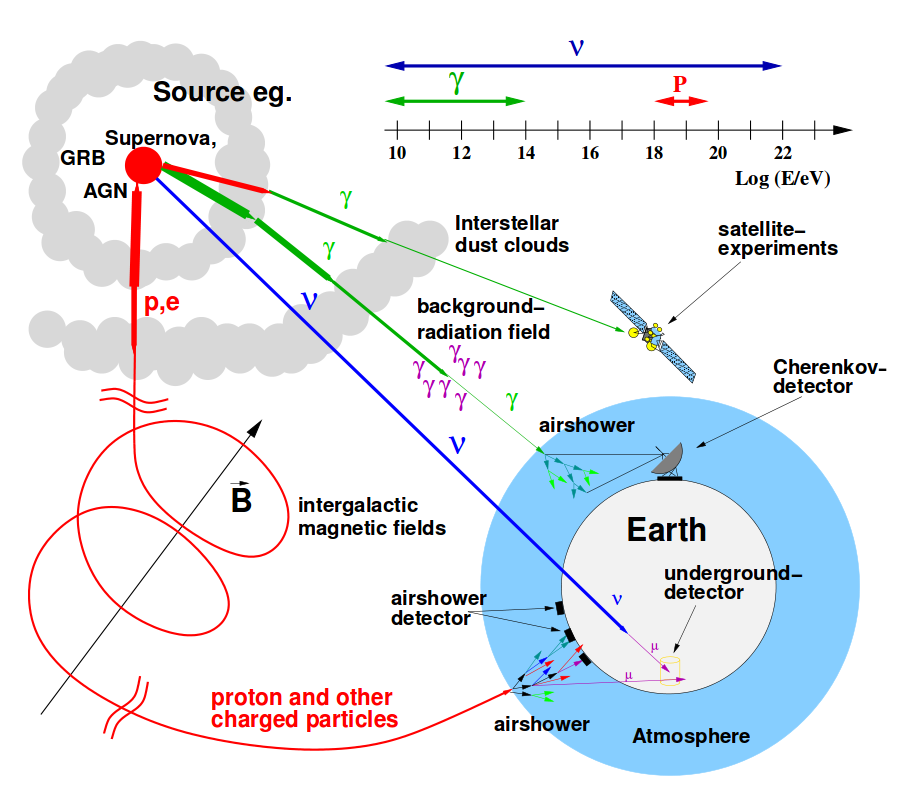
\includegraphics[width=0.8\textwidth]{./Plots/02_Astroteilchenphysik/Astroteilchen.png}
    \caption{Auf dem Weg von der Quelle zum Beobachter unterliegen die unterschiedlichen Botenteilchen unterschiedlichen Wechselwirkungen. 
    Geladene Teilchen wechselwirken mit Staubwolken und werden von Magnetfeldern abgelenkt, Neutrinos und hochenergetische Photonen behalten ihre Richtungsinformation bei.
    Photonen wechselwirken ebenfalls mit Staubwolken oder mit niederenergetischen Hintergrundphotonen und werden dann abhängig von ihrer Energie mit unterschiedlichen Detektoren detektiert. 
    Das Bild entstammt \cite{DissMarlene}.}
    \label{Astroteilchen}
\end{figure}


\autoref{Astroteilchen} zeigt eine schematische Darstellung der verschiedenen Botenteilchen, die von einer astrophysikalischen Quelle emittiert werden können.

Geladene Teilchen wie z.B. Protonen oder Elektronen werden aufgrund ihrer Ladung auf ihrem Weg von der Quelle zum Beobachter von Magnetfeldern abgelenkt und verlieren damit ihre Richtungsinformationen.

Neutrinos hingegen können wegen ihrer geringen Wechselwirkungswahrscheinlichkeit diese Strecke ungehindert zurücklegen. 
Allerdings ist ihre Detektion schwierig.
Detektoren mit großem Volumen können sie indirekt z.B. über Myonen detektieren.

Hochenergetische Photonen besitzen den gleichen Vorteil wie Neutrinos und werden auf dem Weg zum Detektor nicht abgelenkt.
Allerdings wechselwirken sie mit Staubwolken oder Hintergrundphotonen, sodass sie abhängig von ihrer Energie mit Satellitenexperimenten direkt oder über Luftschauerteleskope indirekt detektiert werden können.

\subsection{Geladene kosmische Strahlung}
Die geladene kosmische Strahlung wurde Anfang des 20. Jahrhunderts mit Hilfe von Ballonexperimenten entdeckt \cite{Hess}.
Aufgrund der Tatsache, dass mit steigender Höhe die Ionisation zunahm, schlossen Hess und Kohlhörster, dass die von ihnen detektierte Strahlung aus dem Weltraum kommen müsse. \cite{Kohlhoerster}
Diese Strahlung besteht zu 85\% aus Protonen, zu 12\% aus $\alpha$-Teilchen und 3\% aus Elementen mit größerer Kernladung.\cite{Grupen}
Das Energiespektrum dieser kosmischen Strahlung ist auf einem sehr großen Energiebereich bekannt und wurde sowohl mit erdgebundenen als auch mit Satellitenexperimenten bestimmt.


\begin{figure}
    \centering
    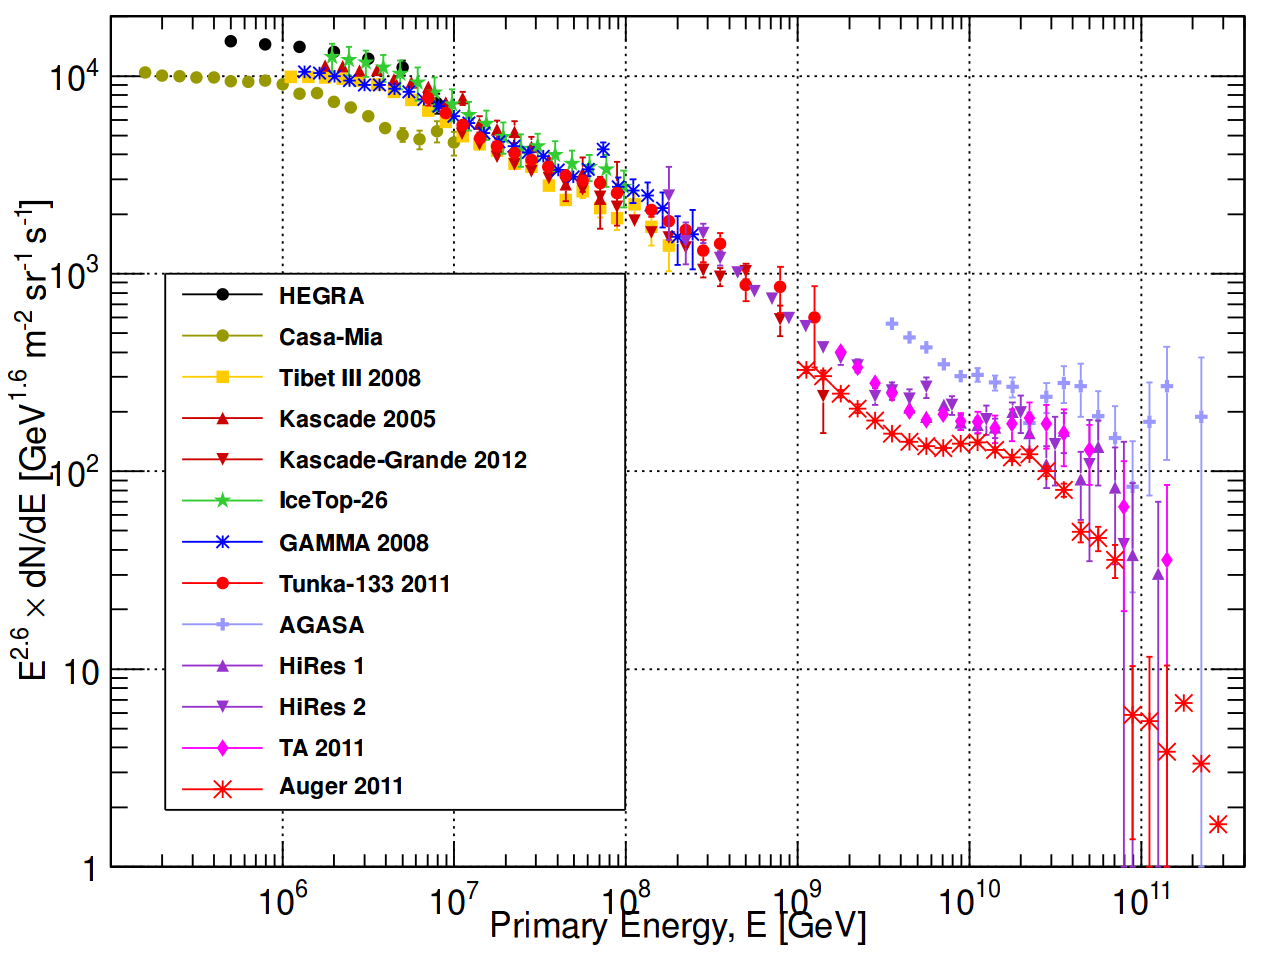
\includegraphics[width=0.8\textwidth]{./Plots/02_Astroteilchenphysik/CosmicRaySpectrum.png}
    \caption{Spektrum der kosmischen Strahlung: Bei der Energie $E=10^{6.4}\,\si{GeV}$ befindet sich das sogenannte "Knie" und bei der Energie $E=10^{9.5}\,\si{GeV}$ die "Ferse" des Spektrums. \cite{GaisserSpektrum}}
    \label{CR-Spektrum}
\end{figure}



Wie in \autoref{CR-Spektrum} zu erkennen ist, kann das Spektrum mit einem gebrochenen Potenzgesetz mit zwei Steigungsänderungen, die als "Knie" und "Ferse" bezeichnet werden, beschrieben werden \cite{DissBecker}:

\begin{equation}
 \frac{dN}{dE_{CR}} \propto E_p^{-\alpha_{CR}}
\end{equation}

mit 

\begin{equation*}
\alpha_{CR}=	
\left\{
\begin{aligned}
2,67 \qquad \log\left( \frac{E_{CR}}{eV} \right) &< 15,4 \\
3,10 \qquad \log\left( \frac{E_{CR}}{eV} \right) &< 18,5 \\ 
2,75 \qquad \log\left( \frac{E_{CR}}{eV} \right) &> 18,5.
\end{aligned}
\right.
\end{equation*}

Größere Energien als $5 \cdot 10^{19} \si{eV}$ können aufgrund des GZK-Cutoffs \cite{Greisen}\cite{ZatsepinKuzmin} nicht gemessen werden. 
Dieser Cutoff tritt auf, wenn Protonen mit dem kosmischen Mikrowellenhintergrund (CMB) wechselwirken \cite{DissBecker}: 

\begin{equation*}
p\gamma_{CMB}=	
\left\{
\begin{aligned}
& \Delta^+ \\
& p e^+ e^- .
\end{aligned}
\right.
\end{equation*}

Knie und Ferse beinhalten Informationen über die Beschleunigungsmechanismen der Teilchen, bzw. über die Quellen.
Die Teilchen mit den höchsten Energien, jenseits der Ferse können nicht galaktischen Ursprungs sein, da die galaktischen Magnetfelder für die Beschleunigung zu schwach sind. 
Deswegen wird vermutet, dass diese Teilchen extragalaktischen Ursprungs sind, wobei die Beschleunigungsmechanismen (vgl. \autoref{sec:Beschleunigungsmechanismen}) noch nicht genau bekannt sind.

\subsection{Neutrinos}
Neutrinos sind leichte Teilchen, die eine sehr geringe Wechselwirkungsqahrscheinlichkeit haben und so in großen Experimenten wie IceCube\cite{Icecube} oder ANTARES\cite{ANTARES} indirekt über Myonen nachgewiesen werden.
Das größte Problem bei der Suche nach hochenergetischen Neutrinos ist der Untergrund, der in Wechselwirkungen von geladener kosmischer Strahlung in der Atmosphäre entsteht.
Neutrinos werden in hadronischen Reaktionen erzeugt und können auf dem Weg von der Quelle zum Detektor oszillieren.
Die Produktion von Neutrinos geschieht über die Produktion von geladenen Pionen und folgende Reaktionen sind möglich:
Entweder wechselwirkt ein Photon mit einem Proton folgendermaßen mit der angegebenen Wahrscheinlichkeit\cite{DissBecker}:

\begin{equation*}
p\gamma \rightarrow \Delta^+ \rightarrow	
\left\{
\begin{aligned}
& p \pi^0 \qquad [2/3] \\
& n \pi^+ \qquad [1/3]
\end{aligned}
\right.
\end{equation*}

oder ein Proton wechselwirkt mit einem anderen Proton\cite{DissBecker}:

\begin{equation*}
p p \rightarrow
\left\{
\begin{aligned}
& p p \pi^0 \qquad [2/3] \\
& p n \pi^+ \qquad [1/3].
\end{aligned}
\right.
\end{equation*}

Die gleichen Prozesse treten auch für Neutronen oder bei höheren Energien Kaonen als Primärteilchen auf, wodurch negativ geladene Pionen entstehen.
Die Pionen zerfallen dann und erzeugen weitere Neutrinos \cite{DissBecker}:

\begin{equation*}
 \begin{aligned}
 \pi^+ \rightarrow \mu^+ \nu_{\mu} \rightarrow e^+ \nu_e \overline{\nu}_{\mu} \nu_{\mu} \\ 
 \pi^- \rightarrow \mu^- \overline{\nu}_{\mu} \rightarrow e^- \overline{\nu}_e \nu_{\mu} \overline{\nu}_{\mu}
 \end{aligned}
\end{equation*}

Aufgrund der beschriebenen Prozesse erwartet man in der Quelle eine Verteilung der Neutrinos von $(\nu_e:\nu_{\mu}:\nu_{\tau})=(\overline{\nu}_e:\overline{\nu}_{\mu}:\overline{\nu}_{\tau})=(1:2:0)$.
Propagieren die Neutrinos Strecken von der Größenordnung des Sonnensystems, oszillieren sie, sodass auf der Erde ein Verhältnis von $(\nu_e:\nu_{\mu}:\nu_{\tau})=(1:1:1)$ beobachtet wird.

Es gibt verschiedene Neutrinoquellen:
\begin{itemize}
 \item Kosmogene Neutrinos werden in Wechselwirkungen von hochenergetischen Protonen mit dem CMB und den darauffolgenden Zerfall von geladenen Pionen erzeugt.
 \item Galaktische Neutrinos können in hadronischen Beschleunigungsprozessen erzeugt werden.
 \item Es wird erwartet, dass in Gamma Ray Bursts Neutrinos erzeugt werden.
 \item In den hadronischen Modellen von AGNs werden Neutrinos produziert. 
\end{itemize}

\subsection{Photonen}
Genau wie die Neutrinos haben Photonen den Vorteil, dass sie nicht von Magnetfeldern abgelenkt werden.
Allerdings könenn aufgrund der Absorption in der Atmosphäre auf der Erde nur Photonen im optischen und im Radiobereich detektiert werden.
Deswegen wurden diese Wellenlängen in der Astronomie auch als erstes benutzt. 
Nach und nach kamen dann die anderen Wellenlängen wie z.B. Röntgenstrahlung oder Gammastrahlung hinzu.
Gammastrahlung lässt sich anhand der Energie in nieder- bis mittelenergetische Gammastrahlung ($\SI{0,1}{MeV}$ - $\SI{30}{MeV}$), hochenergetische Gammastrahlung ($\SI{30}{MeV}$ -$\SI{100}{GeV}$), sehr hochenergetische Gammastrahlung ($\SI{100}{GeV}$-$\SI{100}{TeV}$) und ultrahochenergetische Gammastrahlung ($E>\SI{100}{TeV}$) einteilen.
Der Energiebereich bis ca. 100GeV lässt sich nur mit Satellitenexperimente nachweisen.
Die sehr hochenergetische und die ultrahochenergetische Strahlung lässt sich wiederum mit Hilfe von Luftschauerteleskopen auf der Erde detektieren.\cite{Weekes}

Das Problem der hochenergetischen Photonen ist, dass sie mit den niederenergetischen Photonen der Hintergrundstrahlung (EBL) wechselwirken.
Mit Hilfe von Modellen kann die Absorption von hochenergetischen Photonen aus extragalaktischen Quellen durch diese Hintergrundstrahlung berechnet werden.\cite{Weekes}

In \autoref{sec:Gammaastronomie} wird dann noch näher auf die Gammaastronomie eingegangen und es werden die Wechselwirkungen erklärt, die die Photonen auf ihrem Weg zur Erde, erfahren.


\section{Quellen kosmischer Strahlung}
\label{sec:Quellen}
In diesem Kapitel wird eine Übersicht über die Quellen der kosmischen Strahlung gegeben.

\subsection{Die Galaktische Scheibe und das Galaktische Zentrum}
Die galaktische Scheibe ist die stärkste und erste detektierte Gammaquelle und wurde 1968\cite{GalacticPlane} detektiert.
Im Folgenden werden die Prozesse beschrieben, die die galaktische Gammastrahlung erzeugen:

\begin{itemize}
 \item Kosmische Elektronen erzeugen niederenergetische Photonen durch Bremsstrahlung mit dem Interstellaren Gas.
 \item Hadronen der kosmischen Strahlung produzieren neutrale Pionen, die dann in zwei Photonen mit mittlerer Energie zerfallen.
 \item Kosmische Elektronen überleben eine inverse Comptonstreuung an niederenergetischen Gammaphotonen und erzeugen Photonen mit hohen Energien.
\end{itemize}

Das Galaktische Zentrum enthält mehrere Objekte, wie z.B. junge Supernova-Remnants wie Sgr $A$ East, die hochenergetische Gammastrahlen emittieren.
Das dynamische Zentrum wurde mit der kompakten Radioquelle Sgr $A^*$ assoziiert, welche vermutlich ein supermassives schwarzes Loch ist.
In einem Radius von 10pc um das Galaktische Zentrum befindet sich eine Masse von $3\cdot 10^7$ Sonnenmassen.
Das Satellitenexperiment EGRET hat die Quelle 3EG J1745-2852 detektiert, welche hochenergetische Gammastrahlung emittiert. 
Die Natur dieser Quelle ist noch unbekannt.\cite{GalacticCenter}\cite{Weekes}


\subsection{Supernovae und Supernovaremnants}
Die Explosion eines Sterns wird als Supernova (SN) bezeichnet.
Gammastrahlung, die aus SN kommt, wird entweder in den ersten Sekunden der Explosion als Gammastrahlenausbruch [Gamma Ray Burst (GRB)] detektiert oder als stete periodische Emission des entstandenen Pulsars.
Es ist auch möglich, dass sie der sich ausbreitenden Hülle des ehemaligen Sterns [Supernova Remnant (SNR)] entstammen. 
Diese galktischen Quellen liefern kosmische Strahlung bis zu Energien von $\SI{100}{TeV}$.
SN und SNR vermögen es nicht, Teilchen auf Energien von $10^20\,\si{eV}$ zu beschleunigen.
Somit entstammen Teilchen mit so hohen Energien extragalaktischen Quellen.\cite{Weekes}

Die Beschleunigung der Teilchen erfolgt in Schockwellen.
Das Modell dieser diffusen Schockbeschleunigung liefert ein Potenzgesetz für das Spektrum der beschleunigten Strahlung von $\frac{dN}{dE} \propto E^{-2,0}$.
Dieses Potenzgesetz wird um Effekte während der Propagation durch die Galaxie korrigiert und resultiert in einem Spektrum der kosmischen Strahlung von $\frac{dN}{dE} \propto E^{-2,7}$
Im Allgemeinen sind die Spektra von Supernovae hart und haben einen Cutoff bei ca. $\SI{20}{TeV}$, was auf eine Primärteilchenenergie von einigen TeV schließen lässt.\cite{Weekes}\cite{RhodeFalke}


\subsection{Gamma Ray Pulsars und Binaries}
Pulsare sind rotierende Neutronensterne. 
Das bekannteste Beispiel ist der Crab Pulsar im Zentrum des Krebsnebels.
Dieser Quelltyp wurde vor mehr als 30 Jahren entdeckt und er lässt sich in zwei Kategorien einteilen.
Der erste Typ gewinnt seine Energie durch Rotation und ist im Radiobereich detektierbar und der andere Quelltyp gewinnt seine Energie durch Akkretion von Materie und ist im Röntgenbereich detektierbar.
Pulsare haben Rotationsperioden zwischen einigen Millisekunden und einigen Sekunden.
Vor allem im Gammabereich ist ihre Luminosität hoch und genau wie bei den SN und SNRs können ihre Energiespektren durch ein Potenzgesetz beschrieben werden.
Verschiedene Pulsare lassen sich anhand ihrer Spektren voneinander unterschieden; auch unterscheiden sich ihre Lichtkurven in der Position der Peaks bei verschiedenen Wellenlängen.
Die Theorie von Pulsaren ist noch nicht komplett verstanden, weswegen Modelle getestet werden.\cite{Weekes}

Die Hälfte aller Sterne taucht in einer Assoziation mit einem anderen Objekt auf und wird Binaries genannt.
Dieses andere Objekt ist oft ein kompaktes Objekt wie ein Weißer Zwerg, ein Neutronenstern oder ein Schwarzes Loch.
Hohe Röntgenemission sowie ein zeitlich variables Verhalten sind charakteristisch für diesen Quelltyp.
Dabei kann die Variabilität im Bereich von Millisekunden bis zu Jahren liegen und periodisch auftauchen oder in einzelnen Ausbrüchen, Flares genannt.\cite{Weekes}


\subsection{Gamma Ray Bursts}
Gammastrahlenausbrüche (GRBs) wurden während des kalten Kriegs von den amerikanischen Vela-Satelliten, die Atombombenexplosionen aufspüren sollten, entdeckt.
16 GRBs mit Zeitspannen von $\SI{0,1}{s}$-$\SI{30}{s}$ mit Flüssen zwischen $(10^{-5}-10^{-4}\,\frac{\si{erg}}{\si{s}}$ wurden detektiert.
Allgemein dauern GRBs zwischen Millisekunden und einigen tausend Sekunden und sind isotrop verteilt.
Sie werden in kurzzeitige Bursts ($t<\SI{2}{s}$) und den Rest unterteilt.
Fast die gesamte emittierte Energie ist größer als $\SI{50}{keV}$.
Mit Satellitenexperimenten wurden GRBs auch im Gammabereich (bis ca. $\SI{30}{GeV}$) detektiert, der Fluss ist aber sehr niedrig.
Bodengebundene Teleskope, wie z.B. MAGIC haben GRB-Programme, allerdings kam es bisher noch zu keiner richtigen Detektion.\cite{Weekes}


\subsection{Aktive Galaktische Kerne}
Die Klasse der Aktiven Galaktische Kerne (AGN) wird durch ein supermassives schwarzes Loch, welches sich in ihrem Zentrum befindet und Materie akkretiert, gekennzeichnet. 
Anhand ihrer Ausrichtung zum Beobachter und ihrer Emission in den verschiedenen Wellenlängen werden AGNs klassifiziert. 
Eine genauere Darstellung dieses Quelltyps, zu dem auch die in dieser Arbeit analysierte Quelle gehört, wird in \autoref{sec:AGN} gegeben.

\section{Beschleunigungsmechanismen} 
\label{sec:Beschleunigungsmechanismen}
Im Folgenden werden die Beschleunigungsmechanismen vorgestellt, die in den relativsitischen Jets von AGNs oder GRBs relevant sind.
Dafür wird zunächst der Fermi-Mechanismus vorgestellt, mit Hilfe dessen geladenen Teilchen beschleunigt wird.
Danach werden die Prozesse zur Erzeugung, bzw. Abschwächung von hochenergetischer Gammastrahlung beschrieben.
Wegen der geringen Teilchendichte in Jets ($n\leq 10^{-3}\,\frac{1}{cm^3}$) werden Prozesse wie Coulombstreuung oder Bremsstrahlung nicht beschrieben.

\subsection{Fermi-Mechanismus 1. und 2. Art}
Die Fermi-Beschleunigung 1.Art beschreibt die Schockbeschleunigung.
Die in einer SN abgestoßene Hülle repräsentiert eine Schockfront, die sich mit einer Geschwindigkeit $u_1$ durch das Interstellare Medium (ISM) fortbewegt. 
Dahinter strömt das Gas mit einer Geschwindigkeit $u_2$ weg.
Kollidiert nun ein Teilchen, welches sich mit der Geschwindigkeit $c$ bewegt, mit dieser Schockfront und wird dabei reflektiert, so gewinnt es die Energie

\begin{equation}
 \frac{\Delta E}{E}\propto \frac{u_1-u_2}{c}.
\end{equation}

Diese Art der Beschleunigung ist somit linear in der Geschwindigkeit und es können maximale Energien von $\approx 100\si{TeV}$ erreicht werden.\cite{Grupen}\cite{Longair}

Die Fermi-Beschleunigung 2.Art beschreibt die Wechselwirkung eines Teilchens mit Geschwindigkeit c mit magnetischen Gaswolken, die sich mit der Geschwindigkeit u bewegen:

\begin{equation}
 \frac{\Delta E}{E}\propto \frac{u^2}{c^2}.
\end{equation}

Die Fermi-Beschleunigung 2.Art ist somit quadratisch in der Wolkengeschwindigkeit.
Da die Teilchen der kosmischen Strahlung einen Teil ihrer Energie in Wechselwirkungen mit dem interstellaren oder dem intergalaktischen Gas zwischen zwei Kollisioinen wieder verlieren, benötigt dieser Beschleunigungsmechanismus eine minimale Injektionsenergie, oberhalb der Teilchen effektiv beschleunigt werden können.\cite{Grupen}\cite{Longair}


\subsection{Synchrotronstrahlung}
Fliegt ein geladenes relativistisches Teilchen durch ein Magnetfeld, emittiert es ein breites Spektrum an Synchrotronstrahlung.
Der Energieverlust dieses Teilchens mit Masse m, Ladung q, Lorentzfaktor $\gamma$ und der Geschwindigkeit $\beta c$, welches sich mit einem Winkel $\Psi$ zum B-Feld mit der Energiedichte $u_B=\frac{B^2}{8\pi}$ bewegt beträgt:

\begin{equation}
 \left( \frac{dE}{dt} \right)_{Sy} = - \frac{16 \pi c}{3} \left(\frac{q}{mc^2} \right)^2 u_B \beta^2 \gamma^2 sin^2(\Psi).
\end{equation}

Unter der Annahme, dass in relativistischen Jets die abstrahlenden Teilchen sofort in zufällige Richtungen gestreut werden, d.h. dass sie zufällig im Verhältnis zum B-Feld verteilt sind und unter der Annahme, dass die Streuung auf kleineren Zeitskalen als die Synchrotronstrahlung passiert, wird über den Winkel $\psi$ gemittelt.
Das führt dazu, dass der Energieverlust umso größer wird, je größer die Masse ist:

\begin{equation}
 \frac{dE}{dt}\propto m^{-2}, \qquad \text{bzw.} \qquad \frac{d\gamma}{dt}\propto m^{-3}.
\end{equation}

Daraus folgt, dass Elektronen ihre Energie effizienter durch Synchrotronstrahlung verlieren können als Protonen.
Für den gleichen Energieverlust müsste ein Proton $6,2 \cdot 10^9$ mal mehr Energie haben.
Das Problem von Elektronen ist, dass sie nachdem sie zu ultrarelativistischen Energien beschleunigt worden sind, ihre Energie sehr schnell wieder verlieren.
Protonen und schwerere Teilchen können einfacher beschleunigt werden,  müssen aber auf extrem hohe Energien beschleunigt werden, um Photonen mit nennenswerter Energie abstrahlen zu können.

Zudem tritt noch das Problem der Synchrotron-Selbst-Absorption auf, d.h. Photonen werden von relativistischen Elektronen im B-Feld absorbiert.\cite{RelativisticJets}

\subsection{Compton-Streuung}
Die Streuung von relativistischen Elektronen an einem Strahlungsfeldes in extragalaktischen Jets wird Compton-Streuung genannt.
Die Photonenergie wird in Abhängigkeit von der Elektron Ruhe-Masse $m_e c^2$ angegeben: $\epsilon= \frac{h\nu}{m_e c^2}$.\cite{RelativisticJets}
 
In niedrigster Ordnung ist der Energieverlust im Thomson Limit, d.h. $\gamma \epsilon <<1$ gegeben durch:

\begin{equation}
-\left(\frac{d\gamma}{dt} \right) \approx \frac{4}{3} c \sigma_T \frac{u_{ph}}{m_e c^2} \gamma^2
\end{equation}

\begin{center}
 \begin{tiny}
  $\sigma_T$: Thompson-Wirkungsquerschnitt, $u_{Ph}$: Energiedichte des Photonfeldes.
 \end{tiny}
\end{center}

Im Thompson-Limit kommt es zu Photonenergien von $\epsilon_S ~\gamma^2 \epsilon_0 << \frac{1}{\epsilon_0} $, wobei $\epsilon_0$ die Energie des isotropen monoenergetischen Photonfeldes ist.\cite{RelativisticJets}

Für große Elektron- und Photonenergien $\gamma \epsilon > 1$ ist Compton-Streuung unterdrückt.\cite{RelativisticJets}


\subsection{$\gamma\gamma$-Absorption und Paar-Produktion}
Die Wechselwirkung von hochenergetischen Photonen miteinander oder mit weniger energiereichen Photonen ist der einzige relevante Absorptionsmechanismus für Photonen in astrophysikalischen Umgebungen.
Ein Photon mit der Energie $\epsilon_1$ wechselwirkt mit einem Photon mit der Energie $\epsilon_2$ unter dem Winkel $\Theta=cos^{-1}\mu$ und produziert ein $e^+/e^-$-Paar falls:
\begin{equation}
 \epsilon_1 \geq \frac{2}{\epsilon_2 (1-\mu)}.
\end{equation}

VHE-Gammastrahlung aus einer Quelle in kosmologischer Entfernungen wird vom Infrarot- und optischen Hintergrundlicht absorbiert. 
Dieser Prozess wird EBL (Extragalactic Background Light)-Absorption genannt. 
Dieses extragalaktische Hintergrundlicht besteht vorwiegend aus der Infrarot-Emission von Staub aus jungen, sternbildenden Galaxien als auch aus der Infrarot- und der optischen Emission von Sternen.
Das Spektrum und die Intensität des EBL hängen von der kosmologischen Zeit bzw. der Rotverschiebung ab und dadurch wird auch die Opazität für VHE-Gammastrahlung bestimmt.
Wegen der großen Emission innerhalb des Sonnensystems und der Milchstraße ist der EBL schwierig zu vermessen.\cite{RelativisticJets}


\subsection{$\gamma$-Hadron-Wechselwirkungen}
Aufgrund der oft dichten Strahlungsfelder in Jets sind die Wechselwirkungen zwischen relativistischen Hadronen und Photonen wichtig.
Zum einen kann es zu Bethe-Heitler-Paarproduktion und zum anderen zu Photomesonproduktion kommen.\cite{RelativisticJets}

Die Bethe-Heitler-Paarproduktion beschreibt die Reaktion eines Kernteilchens an einem Hintergrund-Photon, wobei ein $e^+/e^-$-Paar entsteht:
\begin{equation}
 p \gamma \rightarrow p' e^+ e^-.
\end{equation}

Diese Reaktion tritt auf, sobald die Schwerpunktsenergie groß genug ist:
\begin{equation}
 s \geq (m_p c^2 +2 m_e c^2)^2 \approx 0,882\si{GeV^2}.
\end{equation}

Die Photomesonproduktion von z.B. Pionen tritt auf, sobald die Schwerpunktsenergie $s \geq (m_p c^2 +2 m_{\pi^0} c^2)^2 \approx \SI{1,16}{GeV^2}$ überschreitet.
Dominant ist die Pion-Produktion in photohadronischen Interaktionen, wobei die $\pi^0$ mit einer Halbwertszeit von $t_{1/2}\approx 8,4\cdot 10^{-17}\,\si{s}$ in zwei Photonen zerfallen und die geladenen Pionen nach einer Halbwertszeit von $t_{1/2}\approx 2,6\cdot 10^{-8}\,\si{s}$ in Myonen und Neutrinos.
Die Produktion und der Zerfall von Kaonen und $\eta$-Mesonen trägt (10-20)\% zur gesamten Photonen-, Leptonen- und Neutrinoproduktion bei.\cite{RelativisticJets}

\subsection{Photodisintegration}
Für Protonen ist der Verlust durch Photomesonproduktion dominierend gegenüber der Bethe-Heitler-Paarproduktion. 
Photodisintegration ist vernachlässigbar.
Photodisintegration beschreibt die Anregung eines Kerns durch ein Photon.
Bei der Abregung wird ein ein oder mehrere Protonen oder Neutronen oder Alpha-Teilchen sowie ein oder mehrere Photonen.
Der Wirkungsquerschnitt hat eine Resonanz ("giant dipole resonance") der Höhe $\sigma_{A\gamma}\approx A \si{mb}$.\cite{RelativisticJets}

\subsection{Elektromagnetische Kaskaden}
In einer photohadronischen Quelle ist die Lichtundurchlässigkeit für primäre Gammastrahlung aus $\pi^0$-Zerfällen oder Compton-Streuung groß, weil sonst keine photohadronischen Wechselwirkungen stattfinden würden.
Solche primären Photonen verursachen eine elektromagnetische Kaskade aus Paarproduktion, Synchrotronstrahlung, Comptonstreuung und Bremsstrahlung.
Dieser Prozess kann innerhalb Jets auftreten, sobald die Photonen genug Energie für die Paarproduktion besitzen und die Dichte an Umgebungsphotonen hoch genug ist.
Sobald die Energie der Photonen nicht mehr ausreichend für die Paarproduktion ist, verschwindet die Kaskade.\cite{RelativisticJets}


\section{Gammaastronomie}
\label{sec:Gammaastronomie}


\begin{figure}
    \centering
    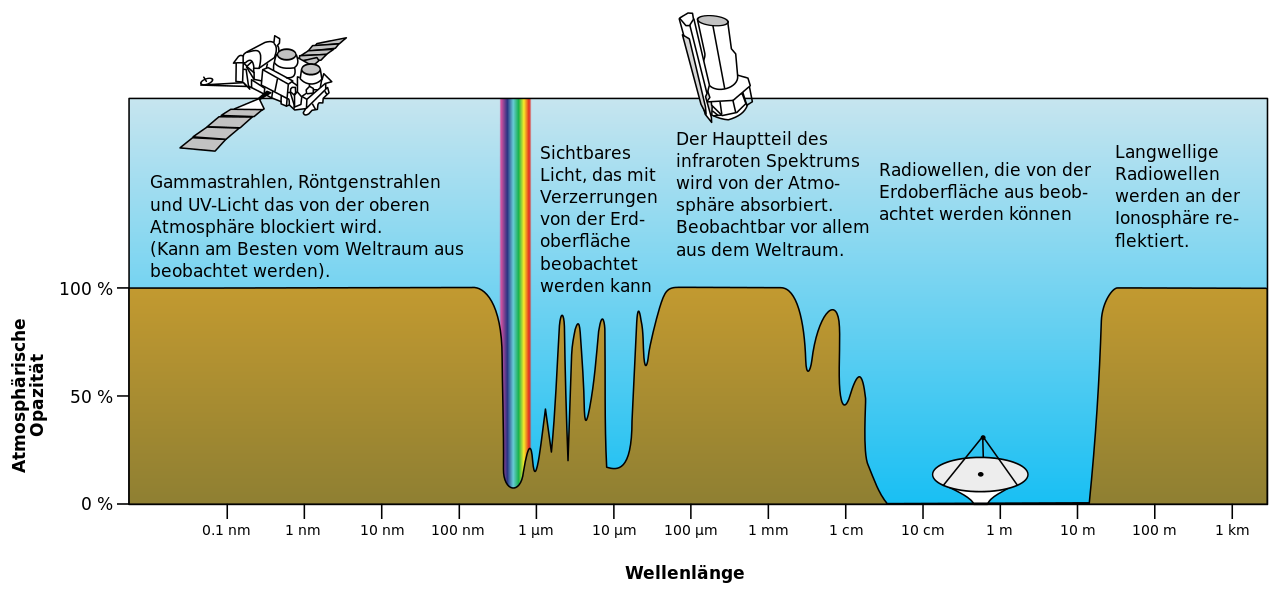
\includegraphics[width=0.99\textwidth]{./Plots/02_Astroteilchenphysik/Atmospheric_electromagnetic_opacity.png}
    \caption{Zu sehen ist die Durchlässigkeit der Atmosphäre für elektromagnetische Strahlung in Abhängigkeit von der Wellenlänge.\cite{Opazitaet}}
    \label{EM-Opazitaet}
\end{figure}


Wie in \autoref{EM-Opazitaet} zeigt, ist die Atmosphäre transparent für optische Beobachtungen und Radiowellen. 
Alle anderen Wellenlängen werden von der Atmosphäre geblockt, sodass bis 1960 nur in diesen Wellenlängen beobachtet wurde.
Mit der Entwicklung der Raumfahrt konnten dann auch Satellitenexperimente konzipiert werden, mit denen Gammaastronomie betrieben wurde.
Aber auch mit bodengebundenen Experimenten wird Gammaastronomie betrieben mit Hilfe von Sekundärprodukten, die mit der Atmosphäre wechselwirken.
Die minimale Energie, bei der Gammastrahlung auf der Erde detektiert werden kann ist zufällig genau über der maximalen Energie, die von Satellitenexperimenten beobachtet wird.
Die bodenegebundenen Experimente beruhen auf der Detektion des Cherenkovlichts von elektromagnetischen Schauern in der Atmosphäre.\cite{Weekes}

Die bevorzugte Wechselwirkung eines Gammateilchen, das mit einer Energie $E>\SI{10}{MeV}$ in die Atmosphäre eintritt, ist die Paaarproduktion, die meist nach einer durchlaufenen Strecke von ca. $\SI{20}{km}$ auftritt.
Das produzierte $e^+/e^-$-Paar fliegt in die gleiche Richtung wie das primäre Photon und wechselwirkt mit den Molekülen der Atmosphäre.
Dabei werden Bremsstrahlungsphotonen emittiert, die dann eine weitere Paarproduktion auslösen können.
Die resultierende Kaskade ist relativ schmal und bewegt sich in die gleiche Richtung wie das Ursprungsteilchen.
Sie wächst so lange bis die Energie der geladenen Teilchen so gering ist, dass Ionisationsverluste und Strahlungsverluste gleich groß sind und erreicht da ihr Schauermaximum.
Danach nimmt die Anzahl der Teilchen der Kaskade ab und der Schauer stirbt aus, was meistens über dem Erdboden passiert.
Die sekundären geladenen Teilchen im Schauer emittieren Cherenkovlicht in Vorwärtsrichtung unter einem Winkel von ca. 1,3°, welches dann von den Teleskopen detektiert wird.
Nicht nur primäre Photonen können solch einen Schauer induzieren, sondern auch Hadronen, wobei der Schauer kein rein elektromagnetischer ist. 
Ein hadronischer Schauer unterscheidet sich in seiner Form von einem elektromagnetischen (siehe \todo{CORSIKA-Referenz}).\cite{Weekes}

Für die Detektion wird ein Detektor mit schneller Elektronik benötigt, mit dem Ziel den Ursprung des Schauers, die Energie und die Ankunftszeit zu bestimmen.
Die Photonenanzahl im Schauer ist ein gutes Maß für die Energie des ursprünglichen Photons.
Für eine große Sensitivität muss die Lichtsammelfläche eines Telskops möglichst groß sein. 
Die Entwicklung von Teleskopen mit segmentierten Spiegeln begann mit dem Whipple-Teleskop\cite{Whipple}.
Heute nutzen sowohl MAGIC\cite{MAGIC_Telescopes}, als auch HESS\cite{HESS} und VERITAS\cite{VERITAS} diese Technologie.
Mit Hilfe von Photomultipliern (PMTs) wird eine hohe Sensitivität für blaue Wellenlängen bereitgestellt. 
Problematisch ist, dass diese PMTs bei zu hellen Bedingungen nicht betrieben werden können und so eine Observation bei Vollmond nicht möglich ist.\cite{Weekes}

Für einen guten Standort muss auch das Störlicht minimiert werden. 
Dies kann durch eine geschickte Standortwahl z.B. auf hohen Bergen fernab von Städten gewährleistet werden.


\section{Aktive galaktische Kerne}
\label{sec:AGN}

\begin{figure}
    \centering
    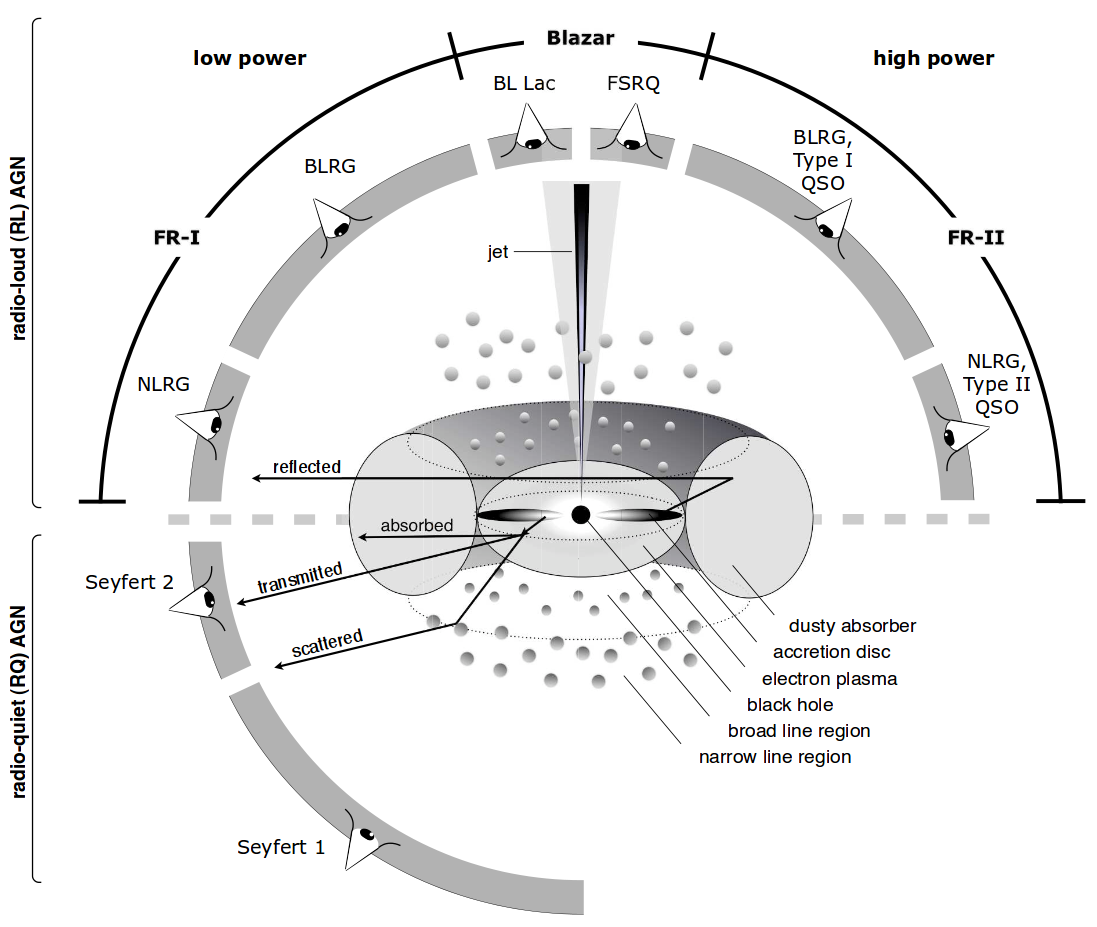
\includegraphics[width=0.8\textwidth]{./Plots/02_Astroteilchenphysik/AGN_Schema.png}
    \caption{Schematische Darstellung einer AGN. Abhängig von der Radioemission und dem Blickwinkel werden die einzelnen AGN-Typen voneinander unterschieden.
    Im Inneren befindet sich ein supermassives schwarzes Loch, welches von einer Akkretionsscheibe umgeben ist. 
    Diese wird wiederum von einem Staubtorus umschlossen.
    Aus dem Zentrum werden zwei entgegengesetzte Jets emittiert.\cite{AGNSchema}}
    \label{AGN_Bild}
\end{figure}

Wie in \autoref{AGN_Bild} zu sehen ist, befindet sich im Zentrum jeder AGN ein supermassives schwarzes Loch, welches Materie akkretiert und eine Akkretionsscheibe formt.
Oberhalb der Scheibe befinden sich Wolken, die mit schneller Geschwindigkeit rotieren und Emissionslinien fabrizieren. Diese Region wird Broad Line Region (BLR) genannt.
Wolken die mit einem größeren Abstand um das schwarze Loch kreisen produzieren die narrow lines und werden Narrow Line Region genannt.
Die BLR und die zentrale Region sind von einem Staubtorus umgeben.
Senkrecht zur Scheibe werden zwei Jets in entgegengesetzte Richtungen emittiert.\cite{Weekes}

\subsection{Klassifikation}
Nach Urry und Padovani\cite{Urry_Padovani} werden AGNs in radiolaute und radioleise Vertreter unterteilt. 
Diese werden dann wieder gemäß ihrer Ausrichtung zur Sichtlinie des Beobachters weiter klassifiziert.
Für eine genauere Informationen siehe \cite{Urry_Padovani}.
Gemäß dieser Klassifikation werden nun Blazare betrachtet.
Bei diesem AGN-Typ handelt es sich um radiolaute Quellen und der Beobachter guckt in den Jet. 
Blazare können in allen Wellenlängen beobachtet werden, d.h. über die volle Breite des elektromagnetischen Spektrums, was ca. 19 Dekaden in der Energie entspricht.
Sie zeichnen sich durch ihre hohe Luminosität im Gammawellenlängenbereich und große Variabilität in allen Wellenlängen aus.
Des Weiteren können starke Korrelationen zwischen den Wellenlängen beobachtet werden.\cite{Weekes}

\subsection{Spektrale Energieverteilung}
Die spektrale Energieverteilung [Spectral Energy Distribution (SED)] beschreibt die Emission einer Quelle aufgeteilt nach den verschiedenen Wellenlängen.
Die SEDs von Blazaren besitzen eine charakteristische 2-huppelige Struktur.
Bei sehr hochenergetischen Blazaren, wie Mrk 421 und Mrk 501 befindet sich der erste Peak bei Röntgenenergien und der zweite Peak bei ca. (10-250)$\si{GeV}$.
Beide Peaks sind vergleichbar hoch.\cite{Weekes}


\subsection{Variabilität}
Blazare haben charakteristische Variabilitäten zwischen einigen Minuten und Jahren.
Die erste Detektion eines Flares, also eines außergewöhnlichen Flussanstiegs, in der VHE-Emission einer AGN fand 1994 statt:
Whipple beobachtete einen Flussanstieg von Mrk421 auf das 10fache.\cite{Weekes}\cite{Mrk421_Outburst}

\subsection{Multiwellenlängenbeobachtungen}
Die simultane Beobachtung einer Quelle mit mehreren Teleskopen zur genauen Überwachung der Aktivität in allen Wellenlängen wird Multiwellenlängenbeobachtung (MWL-Beobachtung) genannt. 
Diese Beobachtungen dienen z.B. dazu, die Beschleunigungs-Mechanismen in den Quellen zu verstehen.
Es können Korrelationen der Flüsse in verschiedenen Wellenlängen untersucht werden.
Die erste MWL-Kampagne wurde 1995 organisiert; Ziel war die Quelle Mrk421.\cite{Weekes}

\subsection{Modelle für hochenergetische Gamma-Emission}
Es existieren zwei grundsätzlich verschiedene Ansätze um die hochenergetische Gammaemission zu erklären.
Dies sind zum einen leptonische Modelle und zum anderen hadronische Modelle.
Im Folgenden werden zuerst zwei mögliche leptonische Modelle und anschließend ein hadronisches Modell vorgestellt.

\subsubsection{Leptonische Modelle}
Die Spektrale Energieverteilung (SED) gibt Hinweise auf die Strahlungsmechanismen, die im Inneren eines Jets vonstatten gehen könnten.
Im Inneren eines Jets werden Elektronen durch Schocks beschleunigt. 
Diese Schocks entstehen durch Materie-Ansammlungen, die den Jet mit verschiedenen Geschwindigkeiten durchlaufen.
Die beschleunigten Elektronen verlieren ihre Energie durch Synchrotronstrahlung im Magnetfeld des Jets und produzieren den Synchrotronpeak in der SED.
Die Position dieses Peaks wird durch die Effizient der Schockbeschleunigung und der Cooling-Prozesse, d.h. der Energieverluste bestimmt. 
Im Folgenden werden zwei verschiedene leptonische Modelle vorgestellt.\cite{Weekes}

\subparagraph{SSC}
Im Synchrotron-Selbst-Compton-Modell werden die in Synchrotron-Prozessen abgestrahlten Photonen zu hohen Energien geboostet, die nahe an den Elektronenergien sind.
Im Thomson-Regime können Photonenergien von $E_{\gamma}\approx \gamma^2 h \nu$ und im Klein-Nishine-Regima $E_{\gamma}\approx \gamma m_e c^2$ erreicht werden.\cite{Weekes}

\subparagraph{External Radiation Compton}
Im External-Radiation-Compton-Modell werden sogenannte Saat-Photonen benötigt, die dann invers Compton gestreut werden.
Diese Saat-Photonen werden außerhalb des Jets produziert, z.B. in der Akkretionsscheibe.\cite{Weekes}

\subsection{Hadronische Modelle}
In den Protonmodellen werden die Gamma-Photonen in proton-induzierten Kaskaden produziert. 
Ziel dieser Modelle ist es, zwei Phänome gleichzeitig zu erklären: 
Das sind zum Einen die Produktion von VHE-Gammastrahlung in AGNs und zum Anderen der Ursprung der extragalaktischen kosmischen Strahlung mit Energien von $10^{20}\,\si{eV}$.
Die sehr hochenergetische Gammastrahlung entsteht durch beschleunigte Protonen im Jet mit Energien von bis zu $10^{18}\,\si{eV}$, die dann mit energieärmeren Photonen wechselwirken und Pionen produzieren.
Die erzeugten Pionen zerfallen und lösen dann eine Kaskade aus.
In manchen Modellen wird die Gammastrahlung als Synchrotronstrahlung von sehr energiereichen Protonen emittiert.
Das Problem der hadronischen Modelle ist, dass kurze Zeitvariabilitäten nicht erklärt werden können, da dafür ein sehr schnelles Cooling der Protonen nötig wäre. 
Durch Synchrotronstrahlung können die Protonen nicht schnell genug abgebremst werden.
Kollisionen mit Photonen oder Ionen im Jet wären eine bessere Erklärung.\cite{Weekes}

In jedem Fall können hadronische Modell erst dann als richtig angenommen werden, wenn ein Neutrinofluss, resultierend aus dem Pion-Zerfall detektiert wird.\cite{Weekes}




\section{Markarian 421}
\label{sec:Mrk421}

\begin{figure}
    \centering
    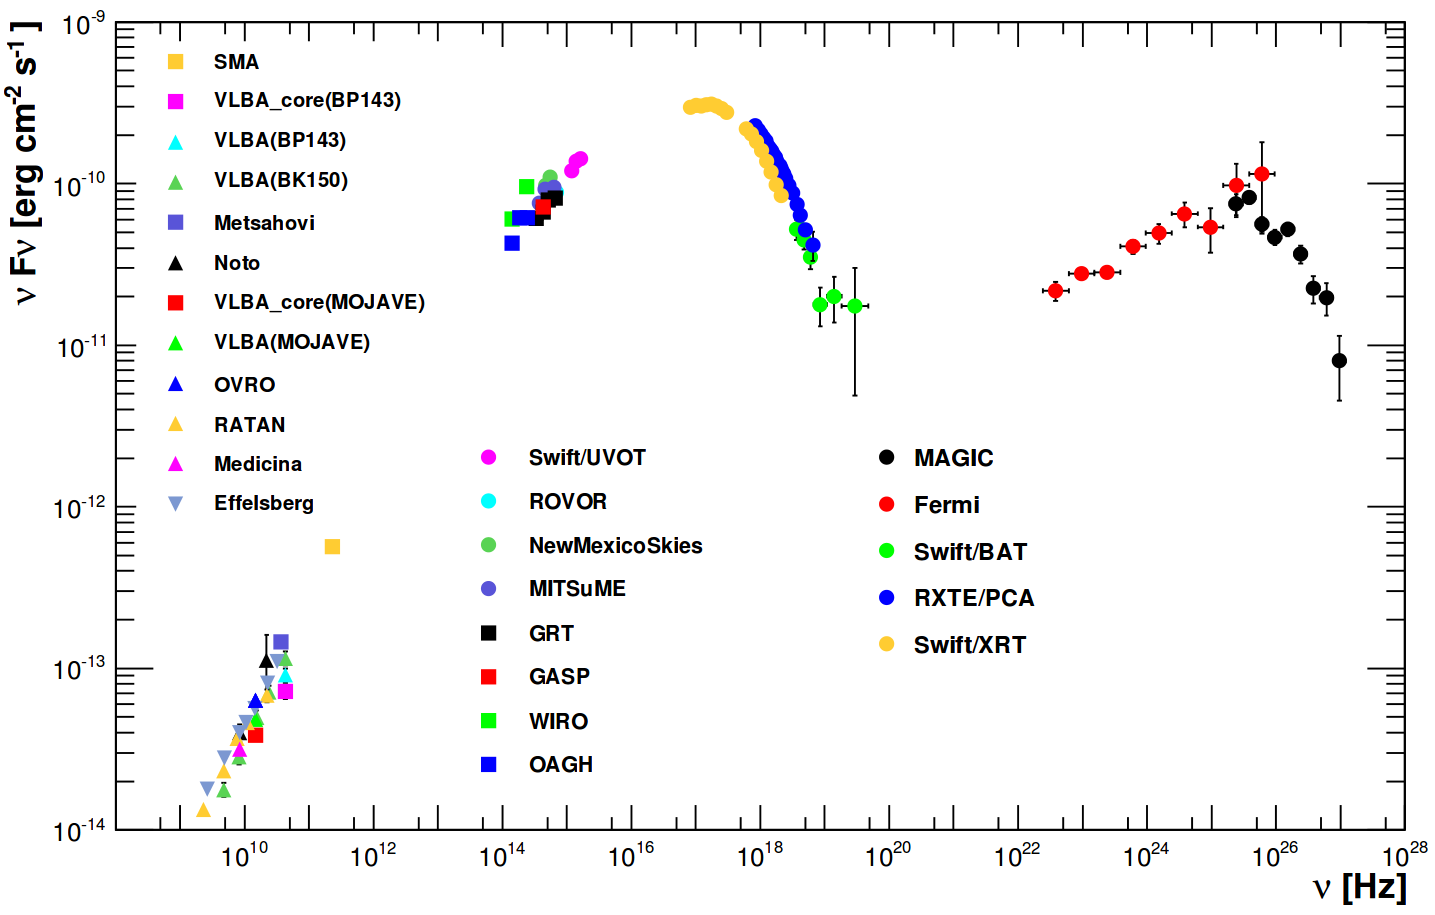
\includegraphics[width=0.8\textwidth]{./Plots/02_Astroteilchenphysik/SED_Mrk421.png}
    \caption{Die Graphik zeigt die SED von Mrk 421. Die für Blazare typische doppelhöckrige Struktur ist erkennbar. 
     Des Weiteren ist zu sehen, dass das Maximum des niederenergetischen und des hochenergetischen Huppels einen ähnlichen Fluss aufweist.\cite{Mrk421_SED}}
    \label{Mrk_SED}
\end{figure}

Die AGN Markarian 421 (Mrk 421) (RA=$11^h 4^m 27,31^s$, Dec=$38°12' 31,8''$) ist eine der hellsten extragalaktischen Quellen im Röntgen- und TeV-Licht und wird dem Typ High Synchrotron Peaked BL Lac zugeordnet.
Sie besitzt eine Rotverschiebung von z=0,0031 und ist damit die nächste Quelle im TeV-Energiebereich.
Neben Mrk 501 ist sie auch die am besten untersuchte Quelle.
Die Quelle ist sehr variabel; so wurde z.B. schon eine Verdopplung des Flusses in $\SI{15}{min}$ beobachtet.
%Es wurden Variationen im Fluss von mehr als einer Ordnung in der Magnitude beobachtet und eine Verdopplung des Flusses in 15min.
Während eines Flares konnte auch eine Änderung in der Steigung des Spektrums beobachtet werden.
In MWL-Kampagnen wurden auch Korrelationen von verschiedenen Wellenlängen beobachtet.
Die charakteristische doppelhöckrige Struktur in der SED ist ebenfalls erkennbar, wobei der erste Peak bei keV-Energien und der zweite bei GeV-TeV-Energien zu erkennen ist (siehe \autoref{Mrk_SED}). 
Mit Hilfe des SSC-Modells kann die Form der SED gut beschrieben werden, wobei hadronische Modelle trotzdem nicht auszuschließen sind.
Die ersten Beobachtungen von MAGIC im Winter 2004/2005 und im Frühling 2005 beinhalten Observationen von Mrk 421.
Eine Multiwellenlängenkampagne von der Quelle hat auch, während die Quelle in einem nicht aktiven Zustand war, Variabilitäten beobachtet und eine Korrelation zwischen VHE und Röntgenstrahlung destgestellt \cite{MWL2009}.\cite{Weekes}
\chapter{Monte Carlo-Simulation}
Ein großes Ziel in der Astroteilchenphysik ist es, Aussagen über die Energiespektren von astrophysikalischen Quellen zu machen.

In dieser Arbeit werden Daten analysiert, die von den beiden MAGIC-Teleskopen aufgenommen wurden, die in Kapitel \ref{sec:MAGIC} kurz beschrieben werden.

In der Datenanalyse sind Monte Carlo (MC)-Daten von grundlegender Bedeutung:
Für die Rekonstruktion eines Energiespektrums einer Gamma-Quelle müssen zunächst einmal Signalevents, die aus der Quelle kommen und Background-Events voneinander getrennt werden.
Dies geschieht heutzutage mit künstlichen Lernalgorithmen, die auf wohl bekannten Beispieldaten, den MC-Daten, trainiert werden müssen.
Auch für die Methode der Entfaltung des Energiespektrums werden MC-Daten benötigt.

Die komplette Produktion der MC-Daten für das MAGIC Experiment wurde im Rahmen dieser Doktorarbeit durchgeführt und wird in diesem Kapitel detailliert beschrieben.

Es werden zunächst die Programme beschrieben, die in der MAGIC MC - Simulationskette genutzt werden.
Angefangen mit der Simulation der Luftschauer mit \textit{CORSIKA} (Kapitel \ref{sec:Corsika}) über die Reflektor-Simulation (Kapitel \ref{sec:Reflector}) wird bis hin zur Kamera-Simulation (Kapitel \ref{sec:Camera}) hier alles beschrieben.
Dabei bauen die Simulationsschritte aufeinander auf, sodass die simulierten Corsika-Events bis zum letzten Schritt weiter prozessiert werden.

Für die eigentlichen Simulationsprogramme (\textit{CORSIKA}, \textit{Reflector} und \textit{Camera}) wird jeweils eine Übersicht über einige wichtige Inputparameter, die den Programmen als text-Dateien,
sogenannten Inputcards, übergeben werden, gegeben.
Nach Abschluss der Simulationskette liegen dann die MC Daten in der gleichen Form vor wie die aufgenommenen Daten der Teleskope. 

Die anschließenden Schritte der Kalibrationskette (\textit{Sorcerer}, \textit{Star} und \textit{Superstar}) von der Signalextraktion und Ankunftszeitbestimmung bis zur Berechnung der Stereo-Bildparameter der gecleanten Events werden in den Kapitel \ref{sec:Calibration} - Kapitel \ref{Superstar} ebenfalls beschrieben.
Diese Kalibration wird im MAGIC Datenzentrum genauso mit den real aufgenommenen Daten durchgeführt, sodass am Ende alle Daten (reale und simulierte) im gleichen Format vorliegen.

Nachdem alle Programme zur Simulation und Kalibration erklärt worden sind, wird auf die automatische Produktionsstruktur auf dem Rechencluster LiDO an der TU Dortmund eingegangen (Kapitel \ref{sec:Automatische MC-Produktion} ).

% \vspace{\fill}


\section{MAGIC}
\label{sec:MAGIC}

Die MAGIC-Teleskope sind zwei IACTs mit einem Spiegeldurchmesser von 17m, die sich auf dem Roque de los Muchachos auf der kanarischen Insel La Palma befinden (siehe Abb.\ref{MAGIC Teleskope}).

\begin{figure}
    \centering
    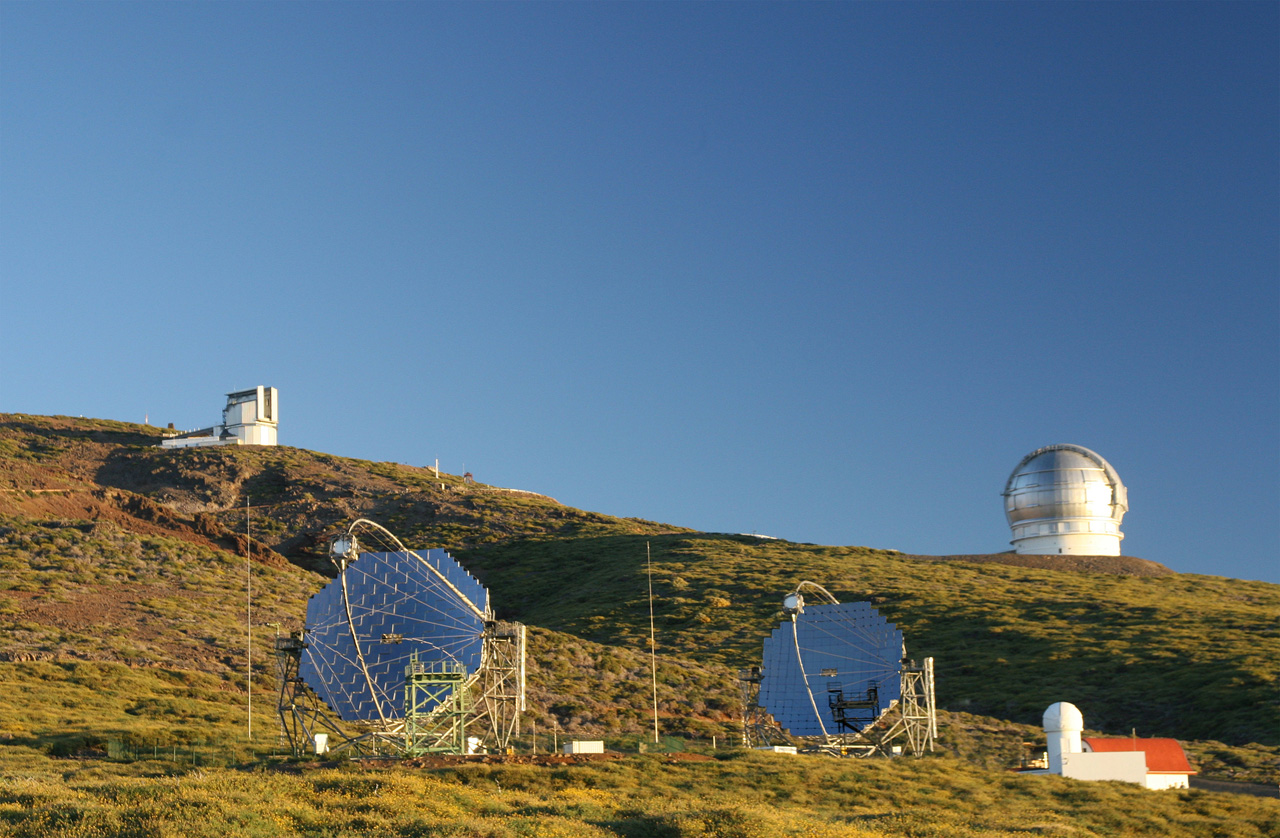
\includegraphics[width=\textwidth]{./Plots/03_MonteCarlos/MAGIC-Telescopes.jpg}
    \caption{MAGIC Teleskope auf dem Roque.[MAGIC Homepage]}
    \label{MAGIC Teleskope}
\end{figure}

Das erste Teleskop -MAGIC I- ist 2004 in Betrieb gegangen und das zweite Teleskop - MAGIC II - 2009.
In den Jahren 2011/2012 wurde ein großes Upgrade des Systems durchgeführt und sehr viel Hardware von MAGIC I durch neuere ersetzt.

Die beiden großen Ziele des Experimentes sind das Erlangen einer niedrigen Energieschwelle und eine schnelle Ausrichtung der Teleskope auf eine Quelle.
Die niedrige Energieschwelle wird durch die große Spiegelfläche, die große Pixelanzahl in der Kamera und die schnelle Ausleseelektronik erreicht.
Durch die leichte Kohlefaser-Struktur der Mounts und die automatische Spiegelausrichtung ist es möglich, das Teleskop schnell und genau auf eine neue Quelle auszurichten.
Es dauert ca 25s, das komplette Teleskop um 180° im Azimuth zu rotieren.

Vor dem großen Kameraupgrade, was im Juni 2012 stattfand, bestand die Kamera von MAGIC I aus 577 Pixeln, unterteilt in 397 innere Pixel mit einem Durchmesser von 1inch und 180 äußere mit einem Durchmesser von 2 inch.
Die Kamera hatte eine hexagonale Form.
Die Kamera von MAGIC II bestand aus 1039 Pixeln mit je 1inch Durchmesser und einem totalen Field of View von etwa 3.5°.
Nach dem Upgrade im Juni 2012 haben beide Teleskope das MAGIC II Kameradesign.

Im Zentrum der Spiegel befindet sich bei beiden Teleskopen die Calibration Box.
Diese sendet sehr kurze Lichtpulse mit konstanter Intensität in Richtung Kamera und dienen der Kalibration der einzelnen Pixel.
Dies geschieht in den sogenannten Calibration Runs oder in den interleaved calibration runs, die während der Datennahme genommen werden.

Das analoge Signal, welches aus den PMTs kommt, wird über optische Fasern zum Trigger und zum Readout im Countinghouise gebracht.

Vor dem Upgrade hab es verschiedene Readout System für MAGIC I und MAGIC II:
Das Readout-System von Magic1 basierte auf dem MUX-FADC-Board, welches robust war und eine gute Performance geliefert hat, allerdings teuer und unhandlich war.
Das Readout-System von Magic 2 basierte auf dem DRS2 Chip, welcher unter recht hohem Rauschen litt.

Nach dem Upgrade wurden beide Auslesesysteme mit dem DRS4-Chip ausgestattet, welcher sich durch wenig Noise, wenig Crosstalk und eine sehr kurze Totzeit auszeichnet.

Der Trigger wird in verschiedene Level unterteilt:
Der Level 0-Trigger ist beinhaltet einen Schwellwert (Discriminator Threshold) für jeden Pixel, die überschritten werden muss, damit ein Event weiterverarbeitet werden kann.
Es folgt der Level 1-Trigger. Dieser basiert auf einem Nächste-Nachbarn-Trigger. 
Für Stereo-Beobachtung müssen 3 nächste Nachbarpixel eines Pixels ebenfalls ein Signal detektiert haben, damit die Level 1-Triggerbedingung erfüllt ist.
Schließlich folgt noch der Stereo-Trigger, welcher die Events auswählt, die in beiden Teleskopen einen Trigger ausgelöst haben und ihren zeitlichen Abstand überprüft.

Diss von Daniel Mazin
Upgrade of the MAGIC Telescopes ICRC
Upgrade Paper I und II


\section{Schauersimulation mit CORSIKA}
\label{sec:Corsika}

CORSIKA wurde am Forschungszentrum Karlsruhe ursprünglich für das KASCADE-Experiment entwickelt und wird heute in vielen Astroteilchenexperimenten eingesetzt.
Mit \textit{CORSIKA} werden ausgedehnte Luftschauer, ausgelöst von kosmischer Strahlung simuliert.

Es können verschiedene Primärteilchen wie Protonen, Eisenkerne oder Photonen als Primärteilchen eingestellt werden.
Diese Primärteilchen werden durch die Atmosphäre propagiert, wo sie Wechselwirkungen mit den Kernen der Luft eingehen und Schauer produzieren oder aber zerfallen.
Die entstandenen Schauer werden dann bis zum Teleskop simuliert.


% \begin{figure}
%     \centering
%     \includegraphics[width=0.3\textwidth]{./Plots/Photon_1TeV_CORSIKA.png}
%     \caption{Schematische Darstellung der automatischestionskette.}
%     \label{CORSIKA_Photon}
% \end{figure}

\begin{figure}
 \begin{subfigure}{0.4\textwidth}
  \includegraphics[width=\textwidth]{./Plots/03_MonteCarlos/Photon_1TeV_CORSIKA.png}
  \caption{Simulation eines Schauers mit 1TeV-Photon als Primärteilchen}
 \end{subfigure}
 \hspace{2.0cm}
  \begin{subfigure}{0.4\textwidth}
  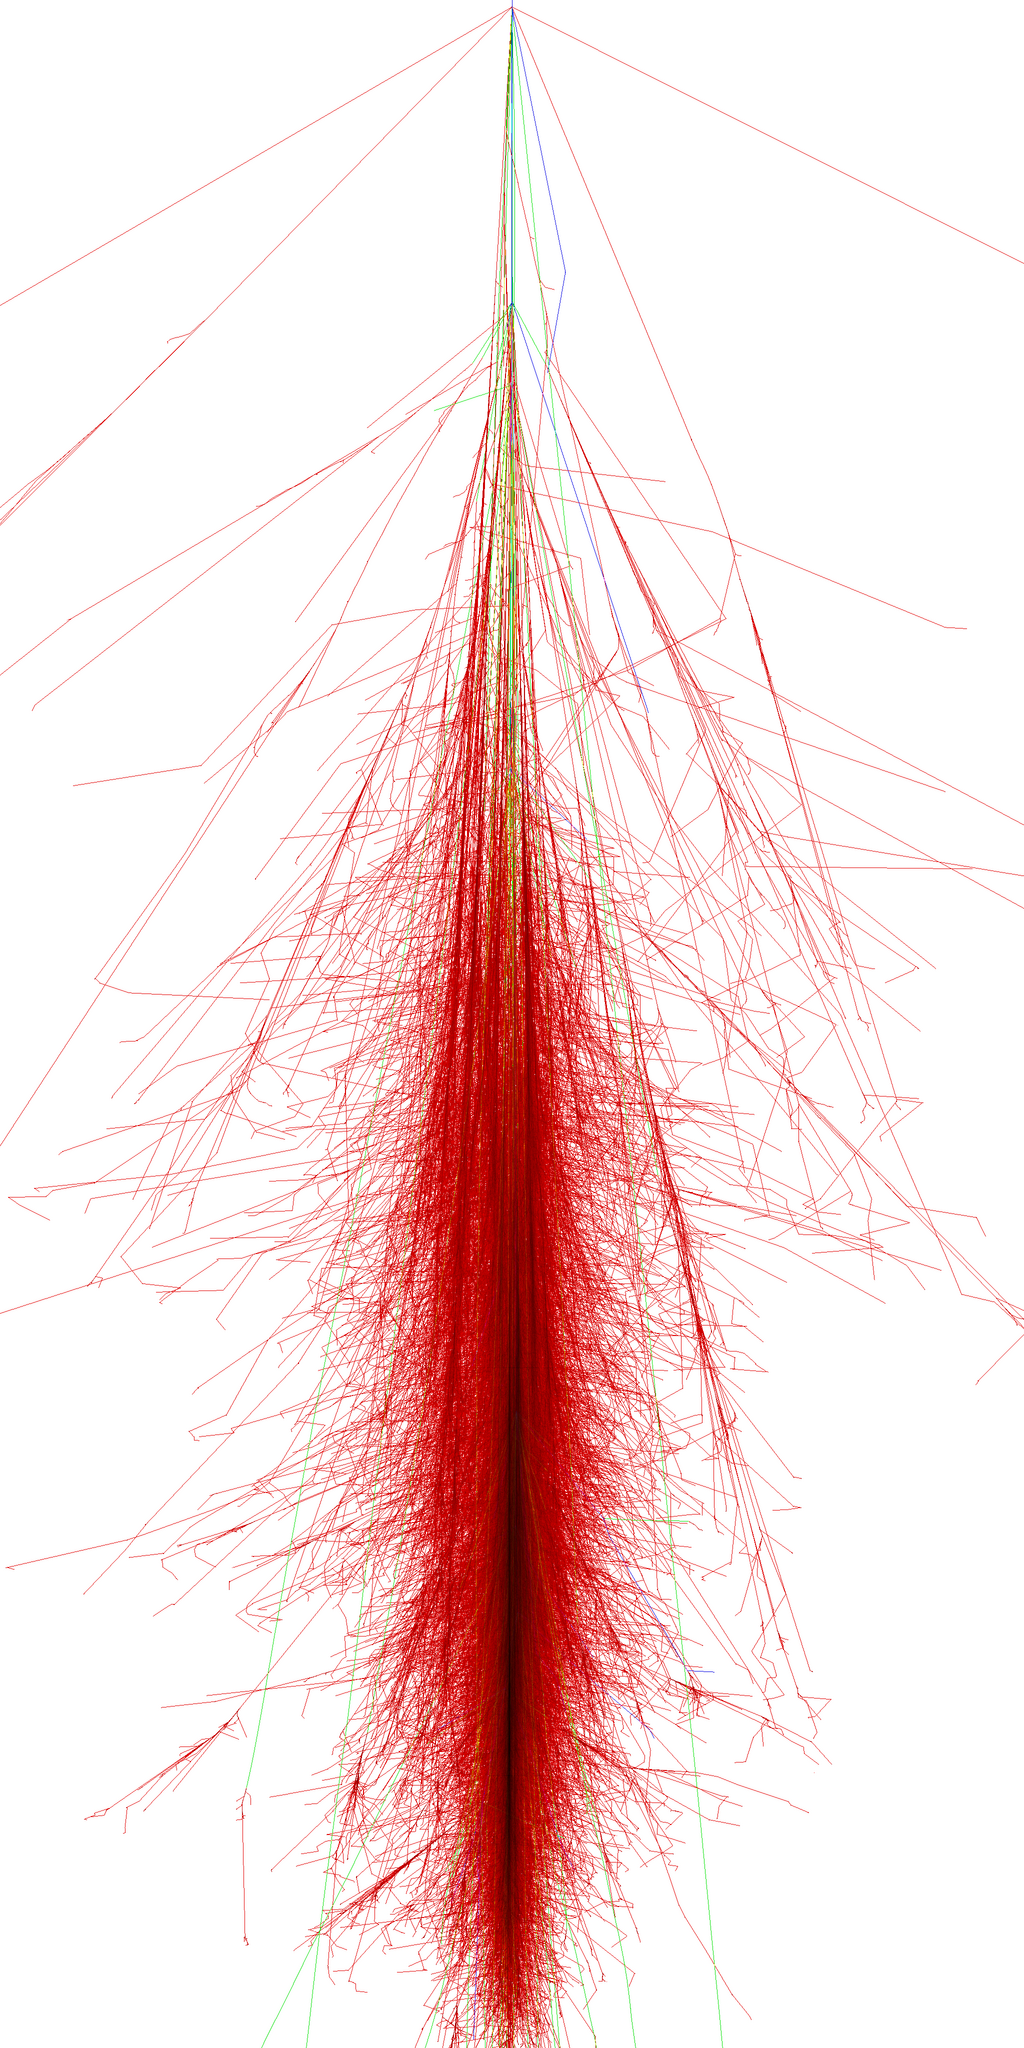
\includegraphics[width=\textwidth]{./Plots/03_MonteCarlos/Proton_1TeV_CORSIKA.png}
  \caption{Simulation eines Schauers mit 1TeV-Proton als Primärteilchen}
 \end{subfigure}
  \caption{ Schauersimulation mit CORSIKA mit 1TeV Primärteilchen}
  \label{CORSIKA_Schauer}
 \end{figure}



In Abb.\ref{CORSIKA_Schauer} sieht man die verschiedenen Eigenschaften der Schauer: Hadronische Schauer haben einen größeren Querschnitt und sind weniger kompakt verglichen mit elektromagnetischen.

Es sind verschiedene Modelle für die hadronische Wechselwirkung bei hohen Energien und bei niedrigen Energien implementiert.
Für die MAGIC MC-Simulation werden QGSJET II für die hadronische Wechselwirkung bei hohen Energien und FLUKA für die Wechselwirkung bei niedrigen Energien benutzt.
Elektromagnetische Prozesse werden mit dem EGS4-Modell beschrieben.
Eine Simulation der Cherenkovphotonen, die von den geladenen Teilchen produziert werden, die durch die Luft propgaieren, erfolgt ebenfalls.

\subsection{Mmcs}
Eine speziell für das MAGIC-Teleskop adaptierte Version von \textit{CORSIKA} wird in der Standardsimulation genutzt.
In dieser Version wurde der Einfluss des Magnetfeldes vor der ersten Wechselwirkung auf das Primärteilchen vernachlässigt um zu verhindern, dass es zu weit vom Teleskop abgelenkt wird.
Außerdem wurde die Simulation der Cherenkovwellenlänge eingebaut und es wurde eingebaut, dass alle Informationen über das Primärteilchen gespeichert werden.

\subsection{Inputcards}
Die Inputcard enthält Informationen über den Teleskopstandort, die simulierten Schauer und über das Magnetfeld.

Zunächst können allgemeine Angaben zur Anzahl der simulierten Events gemacht werden. 
So erhält jeder \textit{CORSIKA}-Run eine eigene Runnumer und die Anzahl der Schauer pro Run wird durch den Parameter \texttt{NSHOW} angegeben.

Außerdem erfolgen noch Einstellungen über die Eigenschaften der Schauer.
Der Parameter \texttt{PRMPAR} gibt die Art des Primärteilchens an und \texttt{ERANGE} beschreibt den Energiebereich, in dem die Primärteilchen simuliert werden.
Die Steigung des Energiespektrums wird mit dem Parameter \texttt{NSLOPE} eingestellt.
Zenit- und Azimutbereich, in dem die Schauer simuliert werden, wer den durch \texttt{THETAP} und \texttt{PHIP} angegeben.

Zudem werden in \textit{CORSIKA} noch Standortangaben zur Geographie des Teleskopstandortes gemacht.
So wird die Höhe über NN im Parameter \texttt{OBSLEV} angegeben und eine Angabe über die horizontale, bzw. vertikale Komponente des Magnetfeldes auf La Palam befindet sich im Parameter \texttt{MAGNET}.
Der Parameter \texttt{ATMOSPHERE} gibt an, welche Parametrisierung der Atmosphäre genutzt wird.

Abgesehen von diesen allgemeinen Angaben gibt es in der Inputcard noch einige Parameter, die dediziert für die Simulation der Cherenkovphotonen sind.
Der Wellenlängenbereich, in welchem Cherenkovphotonen simuliert werden, wird mit \texttt{CWAVLG} angegeben.
Der Impact-Parameter, der angibt, in welcher Entfernung der Schauer vom Teleskop entfernt auftreffen kann, wird mit \texttt{CSCAT} angegeben.
Der Parameter \texttt{CERTEL} beinhaltet Standort und Größe der Teleskope, die man simuliert und mit der Option \texttt{CERFIL} wird angegeben, ob der Output über die Cherenkovphotonen in eine extra Datei geschrieben wird.


% Einige Einstellungen werden im Folgenden beschrieben:
% 
% \begin{itemize}
%  \item Jedem Corsika-Run wird eine eigene Runnummer zugewiesen
%  \item Mit PRMPAR wird die Art des Primärteilchens eingestellt, was simuliert werden soll.
%  \item ERANGE beschreibt den Energiebereich, in dem Primärteilchen simuliert werden.
%  \item Die Anzahl der Schauer pro Run wird durch NSHOW angegeben.
%  \item Es ist möglich, den Slope des Energiespektrums der Primärteilchen mit ESLOPE einzustellen.
%  \item THETAP und PHIP beschreiben den Zenit- und Azimutbereich, in dem die Schauer simuliert werden.
%  \item Die Höhe über NN des Teleskops wird mit OBSLEV angegeben.
%  \item MAGNET gibt die horizontale und die vertikale Komponente des Magnetfeldes auf La Palma an.
%  \item ECUTS sind die Cut-offs in der unteren Energie für Hadronen, Myonen, Elektronen und Photonen.
%  \item MUADDI gibt falls es auf TRUE gesetzt schreibt zusätzliche Informationen über Myonen raus.
%  \item Mit MUMULT kann man einstellen auf welche Art die Myonen gestreut werden.
%  \item LONGI ist ein Parameter für die longitudinale Schauerentwicklung.
%  \item MAXPRT ist die maximale Nummer der gedruckten Events.
% \end{itemize}
% 
% Nun gibt es in der INputcard noch einige Parameter die dediziert für die Simulation der Cherenkovphotonen sind:
% So zum Beispiel:
% 
% \begin{itemize}
%  \item CWAVLG gibt an, in welchem Wellenlängenbereich Cherenkovphotnen simuliert werden sollen.
%  \item Mit CSCAT kann man einstellen, wie oft ein Cherenkovevent wiederbenutzt wird und der Impact ,d.h. der Bereich, in dem der Schauercore vom Teleskop entfernt auftreffen kann.
%  \item Falls CERFIL TRUE ist, wird der Output über die Cherenkovphotonen in ein extra File geschrieben.
%  \item Mit CERTEL gibt man den Standort und die Größe der Teleskope an, für die man simulieren möchte.
%  \item ATMOSPHERE sagt, welche Parametrisierung der Atmosphäre genutzt werden soll.
% \end{itemize}

\section{Simulation des Reflektors mit Reflector}
\label{sec:Reflector}
Wie der Name schon sagt, wird im Programm \textit{Reflector} vor allem der Reflektor simuliert, allerdings kommen noch einige Zusatzfunktionen ins Spiel.

Mit \textit{Reflector} wird zuerst die atmosphärische Absorption der Cherenkovstrahlung in der Luft simuliert. 
Dabei werden Rayleigh-Streuung, Mie-Streuung und die Absorption an Ozon simuliert.
Als nächstes wird mit Hilfe von Ray-Tracing simuliert, ob die Cherenkovphotonen den Teleskopspiegel treffen.
Dort angekommen muss die Absorption der Aluminium-, bzw. Glasspiegel berücksichtigt werden und die Photonen reflektiert werden.
Nach der Reflexion am Spiegel wird nacheinander überprüft, ob die Photonen die Kamera treffen und letztendlich die Ankunftszeiten in der Kamera bestimmt.

\subsection{Inputcards}
Für diese Simulationsschritte werden bestimmte Inputparameter, bzw. Inputdateien benötigt, die die Eigenschaften des Reflektors beschreiben.
Die wichtigsten werden im Folgenden kurz erklärt.

Es muss der Pfad zur \textit{CORSIKA}-Inputdatei sowie die Output-Pfade für die beiden Reflektordateien (je eine pro Teleskop) angegeben werden.

Teleskopstandort und Wobble Position müssen angegeben werden.

Pro Teleskop wird ein \texttt{mirror\_definition\_file} für die verschiedenen Spiegel (Glas und Aluminium) benötigt.
In dieser Datei sind grundlegende Eigenschaften des Teleskops wie zum Beispiel der Abstand zwischen Spiegel und Kamera festgelegt. 
Des Weiteren wird der Kameraradius angegeben und die Anzahl der Spiegel mit ihrer jeweilige Größe.
Für jeden Spiegel sind einzeln ihre jeweilige ID, der Fokalabstand, die Koordinaten des Spiegelmittelpunkts und der Normalenvektor des Spiegels aufgelistet.

Im sogenannten \texttt{reflectivity\_file} sind die gemessenen Reflektivitäten der einzelnen Spiegel aufgelistet.

Das \texttt{axisdev\_file} beschreibt die Abweichung der einzelnen Spiegel von der idealen Pointing Position.

Im \texttt{measuredpsf\_file} ist die gemessene PSF eingetragen.

Letztendlich muss man in Reflector noch das Atmosphärenmodell, welches für die Simulation benutzt werden soll, angegeben werden. 
Aktuell wird das MagicWinter-Modell benutzt. 
Eine Parametrisierung des Modells enthält abhängig von der Höhe die Dichte, die Dicke und der Brechungsindex (siehe Arbeit von Mareijke Haffner).


\section{Simulation von Kamera und Elektronik mit Camera}
\label{sec:Camera}
Das Programm \textit{Camera} simuliert das komplette Verhalten der Kamera inklusive der Beiträge des Nachthimmeluntergrundes (NSB).
Es werden neben den Schauern also auch der diffuse NSB und Sterne im Field of View simuliert. 
Des Weiteren werden der Trigger und das elektronische Rauschen simuliert, sodass bei einer Änderung der Hardware der Kamera, bzw der Elektronik nicht die komplette MC Kette noch einmal durchlaufen werden muss.
In Abb.\ref{Kamera-Bild} befindet sich ein generiertes Cherenkovevent in der Kamera mit einer Energie von $\SI{3.0}{TeV}$.

\begin{figure}
    \centering
    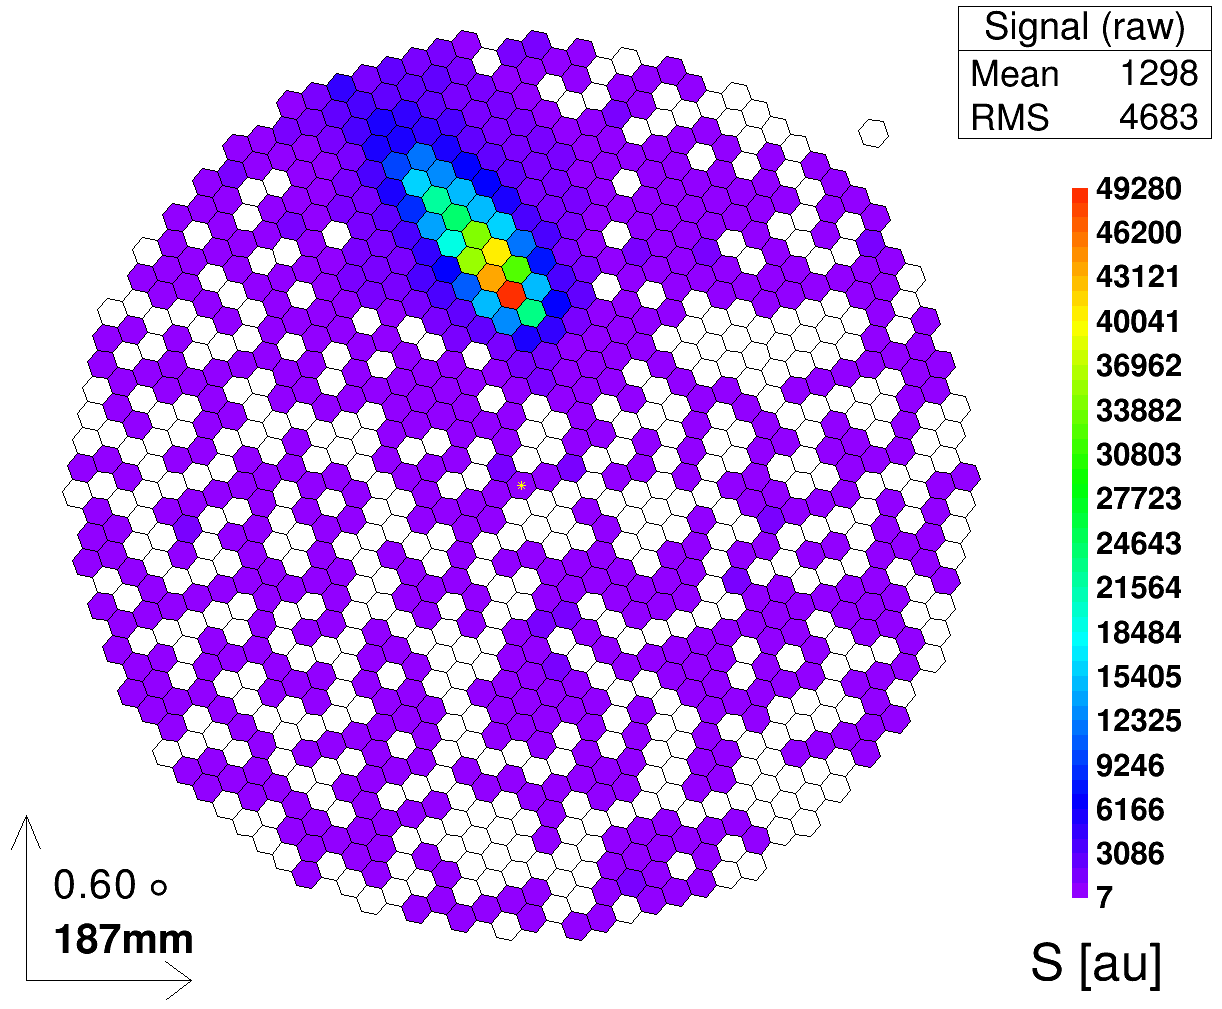
\includegraphics[width=0.6\textwidth]{./Plots/03_MonteCarlos/Signal_Job481_RunNr1513276_511_e3.0TeV_Zd32.2_fertig.png}
    \caption{Darstellung eines simulierten Schauers mit einer Primärteilchenenergie von $\SI{3.0}{TeV}$ in der Kamera. Dargestellt ist der Pixelinhalt in [a.u.].}
    \label{Kamera-Bild}
\end{figure}

Im Folgenden wird die Simulation beschrieben, die mit zwei möglichen vorbereitenden Schritten beginnt: der Simulation des NSB und der Sterne im FoV.

\subsection{StarFieldAdder und StarResponse}
Da MAGIC sensitiv für Sterne bis zur Magnitude 10 ist, tragen die Sterne zum Rauschen in der Kamera bei.
Das Programm \textit{StarFieldAdder} berechnet anhand von einem Katalog, welche Sterne im FoV sind und berechnet dann, wieviele Photonen von diesen Sternen mit welcher Wellenlänge den Spiegel treffen.
Der Output wird im \textit{CORSIKA}-Format geschrieben und muss noch durch \textit{Reflector} laufen, bevor er von \textit{Camera} benutzt werden kann.
Eine Simulation der Sterne im FoV wird in der Standard-MC-Simulation nicht durchgeführt, da die MC-Daten für alle Quellen in einem bestimmten Zenitbereich benutzt werden sollen und nicht für jede Quelle eigene MC-Daten produziert werden.

Um die Simulation zu beschleunigen und damit nicht für jedes Event der diffuse NSB neu berechnen werden muss, wird mit \textit{StarResponse} eine NSB-Datenbank generiert und daraus dann das NSB-Rauschen berechnet, welches dann zusammen mit dem Cherenkovphotonensignal zum Trigger geht.

\subsection{Simulation von Kamera und Elektronik}
Nachdem alle Parameter aus der Inputcard eingelesen worden sind und die individuelle PixelResponse mit NSB gefüllt wurde, erfolgt die eigentliche Verarbeitung der zuvor simulierten \textit{Reflector}-Daten.
Die Photonen aus den Schauern werden eingelesen und für jedes Photon werden folgende Werte einzeln bestimmt:

\begin{itemize}
 \item Pixelization: In welchem Pixel kommt das Photon an
 \item PhE-Produktion: Unter Berücksichtigung der wellenlängenabhängigen Quanteneffizienz jedes PMTs und der Winston Cones wird entschieden, ob ein Photoelektron erzeugt wird.
 \item Channel Response: Für jedes Photoelektron, was die Photokathode verlässt, wird das Analogsignals des PMTs generiert.
\end{itemize}

Danach werden die Signale und Ankunftszeiten aller Photonen eines Pixel superponiert und die Response des Triggers und FADC Systems berechnet und elektronisches Rauschen hinzugefügt.
Das wird für alle Pixel gemacht und man erhält das analoge Signal.
Dann wird durch eine Baseline-Subtraction die AC Kopplung simuliert, die zwischen dem PMT Output und dem Signal ist, welches in den Discriminator Trigger geht.
Danach steht noch die Simulation des Triggers aus. 
Es wird gecheckt, ob das analoge Signal eine bestimmte Schwelle, die Discriminator Schwelle, überschreitet.
Falls ja, wird ein digitales Output Signal simuliert.
Dann wird der first Level Trigger simuliert:
Ob das Event triggert beruht auf seiner Topologie und der Multiplizität.
Dafür wird eine Nächste-Nachbarn-Bedingung überprüft, d.h. die minimale Anzahl an Pixeln, die einen bestimmten Photoneninhalt haben und ihre Verteilung in der Kamera.
Falls diese Bedingungen erfüllt sind, wird ein First Level Trigger Signal generiert und der Output des FADC Systems, welches die digitalisierte Form des analogen Signals ist, wird gespeichert.
Dann wird der nächste Schauer prozessiert.

\subsection{Inputcard}
Im Folgenden werden einige Parameter erklärt, die in der Inputcard von \textit{Camera} enthalten sind.
Wie in jeder Inputcard müssen die Pfade zu den zu prozessierenden \textit{Reflector}-Dateien angegeben sein sowie ein Output-Pfad.
Im Folgenden werden einige Dateien angegeben, die das Programm Camera benötigt:

\begin{itemize}
 \item \texttt{qe\_file}, in welchem die Quanteneffizienz der PMTs als Funktion ihrer Wellenlänge angegeben ist
 \item \texttt{lightcollision.dat}, was die Lichtkollektionseffizienz der Pixel als Funktion des Winkels zwischen Photontrajektorie nach der Reflexion am Spiegel und der Kameraebene angibt.
 In diesem Wert muss die Transmission des Plexiglasfensters der Kamera, die Reflektivität der Winston Cones (Lichtleiter) und die Kollektionseffizienz der Photoelektronen der ersten Dynode der PMTs beinhalten.
 \item \texttt{star\_field\_file}, welches vorher generiert wurde und die Sterne im FoV enthält.
\end{itemize}

Zudem werden einige Parameter, die den NSB betreffen hier eingeführt.
Erst einmal muss definiert werden, ob der NSB simuliert werden soll oder nicht. 
Dies geschieht mit dem Befehl \texttt{nsb\_on}, bzw. \texttt{nsb\_off}.
Des Weiteren muss der Pfad zur vorher generierten NSB Datenbank gegeben werden, was mit dem Parameter \texttt{nsb\_directory} geschieht.
Falls die äußeren (früher größeren) Pixel einen anderen Gain haben, ist dort auch der Einfluss des NSB anders. 
Dies wird durch \texttt{nsb\_dir\_outer} angegeben.
Ein weiterer Parameter, der den NSB betrifft, ist \texttt{nsb\_mean}.
Die erste Zahl gibt die Amplitude des NSB in Anzahl an Photoelektronen pro einem inneren Pixel der Kamera pro ns an.
Wenn man also eine andere Geometrie (größere Spiegel oder größere Pixel) oder eine andere Kamera (andere Quanteneffizienz) simulieren möchte, wird die Photoelektronrate automatisch skaliert.
Die zweite Zahl gibt an, wie groß die Anzahl der Photoelektronen eines Schauers minimal sein muss, damit NSB für diesen Schauer generiert wird.
Die meisten Schauer produzieren wenige oder gar keine Photonen in der Kamera und werden ignoriert.
Für alle Schauer mit weniger als 10 Cherenkovphotonen wird kein NSB produziert, da diese Schauer mit hoher Wahrscheinlichkeit auch nicht getriggert werden.

Der Parameter \texttt{mirror\_fraction} gibt die Zahl der Spiegel an, die zur Reflexion des Lichts beiträgt. 
Mit Hilfe dieses Parameters können fehlende Spiegel in der Simulation berücksichtigt werden.

Der Parameter \texttt{ct\_geom} gibt Aufschluss über die Kamera-Geometrie für jedes Teleskop und beinhaltet Anzahl, Größe und Position der Pixel.

Abgesehen von den oben beschriebenen Parametern gibt es noch zahlreiche weitere, die die Triggereinstellungen und die FADC-Einstellungen betreffen.

Nachdem \textit{Camera} durchgelaufen ist, ist die eigentliche Simulationskette beendet und die Daten liegen im gleichen Format vor wie die real aufgenommenen.
Es erfolgt die gleiche Kalibration wie auch bei den echten Daten und die Einstellungen in den folgenden Programmen unterscheiden sich kaum noch.

% \begin{itemize}
%  \item Pfad zu den beiden Reflectorfile
%  \item qe-file, in welchem die Quanteneffizienz der PMTs als Funktion ihrer Wellenlänge angegeben ist
%  \item Lightcollision.dat, was die LIchtkollektionseffizienz der Pixel als Funktion des Winkels zwischen Photontrajektorie nach der Reflexion am Spiegel und der Kameraebene angibt.
%  In diesem Wert muss die Transmission des Plexiglasfensters der Kamera, die Reflektivität der Winston COnes (Lichtleiter) und die Kollektionseffizienz der Photoelektronen der ersten Dynode der PMTs beinhalten.
%  \item star field file, welches vorher generiert wurde und die Sterne im FoV enthält.
%  \item $nsb_on$, bzw. $nsb_off$ soll NSB simuliert werden oder nicht
%  \item $nsb_directory$: Der Einfluss auf die Elektronik Chain durch NSB wird aus den vorher generierten Dateien genommen. 
%  Mit diesem Befehl gibt man dem Kamera-Programm den Pfad zur vorher generierten NSB-Datenbank 
%  \item $nsb_dir_outer$: Falls die äußeren (früher: größeren) Pixel einen anderen Gain haben als die inneren, ist auch der Einfluss des NSB dort anders.
%  \item $data_file$: Mit diesem Parameter gibt man den Namen des Output Text Files an, in dem eine kurze Triggerstatistik (Anzahl der prozessierten Events und Anteil der getriggerten Events) drin ist
%  \item $root_file$: Name des eigentlichen Output Files von Camera
%  \item $ct_num$: Anzahl der simulierten Teleskope (für uns also 2)
%  \item $ct_geom$: Kamera-Geometrie für jedes Teleskop. Darin enthalten sind Anzahl, Größe und Position der Pixel
%  \item $mirror_fraction$: Die erste Zahl gibt den Teleskopindex an und mit der zweiten Zahl wird die Anzahl der Spiegel angegeben, die zur Reflexion des LIchts beiträgt.
%  Mit Hilfe dieses Inputparameters kann man fehlende Spiegel in der Simulation berücksichtigen.
%  \item $nsb_mean$: Die erste Zahl gibt die Amplitude des NSB in Anzahl an Photoelektronen pro einem inneren Pixel der Kamera pro ns an
%  Wenn man also eine andere Geometrie (größere Spiegel oder größere Pixel) oder eine andere Kamera (andere Quanteneffizienz) simulieren möchte, wird die Photoelektronrate automatisch skaliert.
%  Die zweite Zahl gibt an, wie groß die Anzahl der Photoelektronen eines Schauers minimal sein muss, damit NSB für diesen Schauer generiert wird.
%  Die meisten Schauer produzieren wenige oder gar keine Photonen in der KAmera und werden ignoriert.
%  Für alle Schauer mit weniger als 10 Cherenkovphotonen wird kein NSB produziert, da diese Schauer mit hoher Wahrscheinlichkeit auch nicht getriggert werden.
%  \item $end_file$: Ende der Inputcard: Alles, was dahinter noch steht, wird ignoriert
% \end{itemize}

\section{Calibration}
\label{sec:Calibration}
Ziel der Kalibration ist es, für jeden Pixel die Ladung in Photoelektronen und die Ankunftszeit der Photonen zu bestimmen.
Dafür muss der Lichtpuls extrahiert und die Baseline abgezogen werden.
Die Baseline wird mit Hilfe von pedestal Events bestimmt, also Events mit zufälligem Trigger, welche keine Schauerpulse enthalten sollten und dann in den richtigen Events abgezogen [vgl. Abb.\ref{Kamera-Bild-Pedestal}].
Ziel der Calibration Runs - Events mit bekanntem Lichtpuls - ist es, die Konversionsfaktoren der einzelnen Pixel zu berechnen.

\begin{figure}
    \centering
    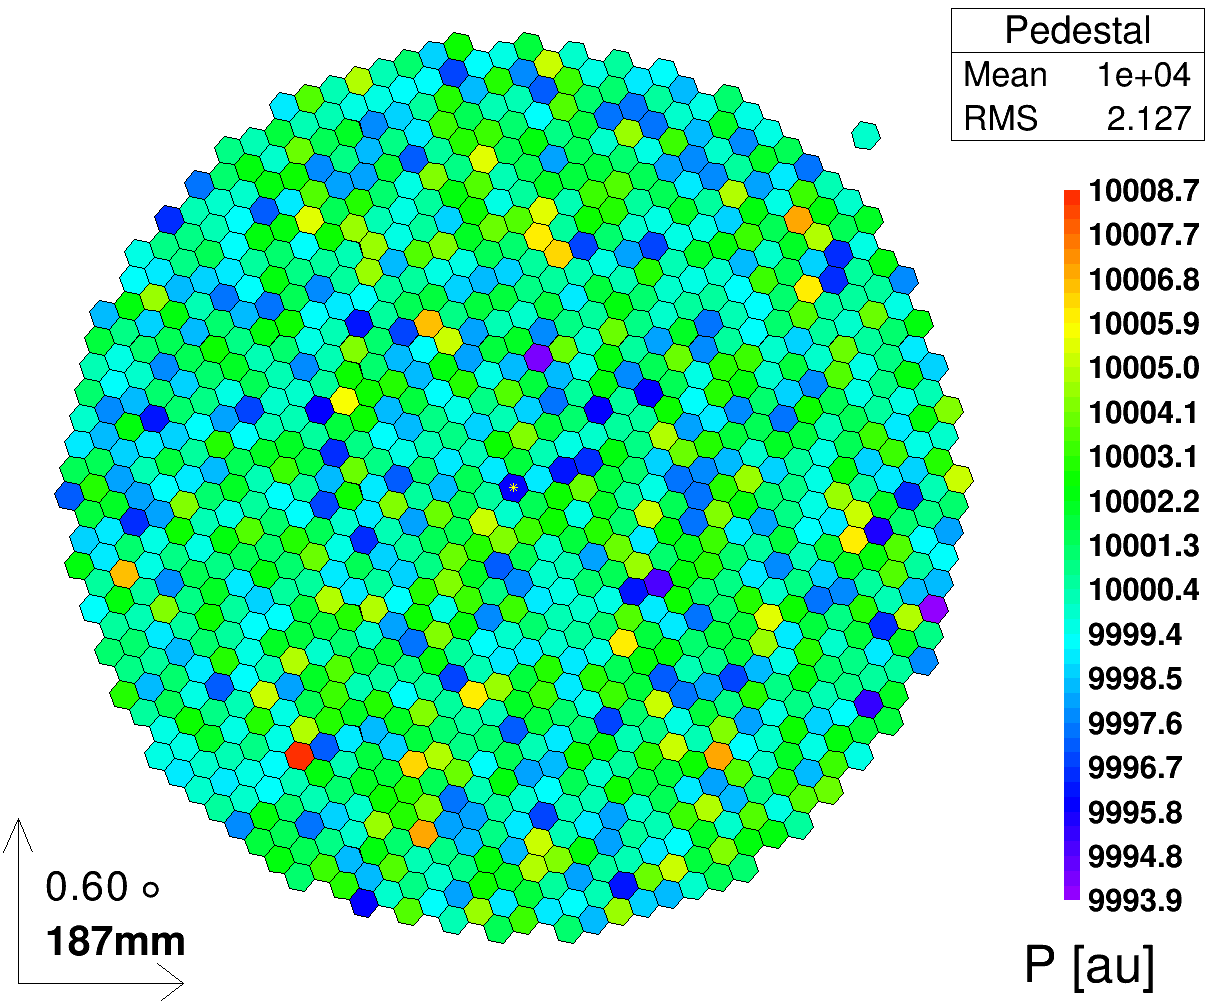
\includegraphics[width=0.6\textwidth]{./Plots/03_MonteCarlos/Pedestal_fertig.png}
    \caption{Darstellung eines simulierten Pedestal Events in der Kamera. Dargestellt ist der Pixelinhalt in [a.u.].}
    \label{Kamera-Bild-Pedestal}
\end{figure}

In der Realität sind Pedestal Events, Events mit zufälligem Trigger und ohne Puls und Calibration Runs sind Runs, die genommen werden, wobei die Calibration Box benutzt wird.
Diese Calibration Box befindet sich im Zentrum der Spiegel und verursacht kurze Lichtpulse mit konstanter Intensität in Richtung Kamera.


\subsection{Signalextraktion}
Ziel der Signalextraktion ist die Integration der Counts in der Pulsregion ohne Baseline.
Dafür gibt es verschiedene Methoden:
\begin{itemize}
 \item Fixed window: Mit dieser Methode wird an einer a priori bekannten Position, an der man den Cherenkovpuls erwartet, über eine bestimmte Länge integriert.
 \item Sliding window: Bei dieser Methode wird das Integrationsfenster so lange verschoben, bis man den Bereich gefunden hat, in dem das Signal am höchsten ist und integriert dort.
 \item Spline: Diese Methode beruht auf der Sliding Window-Methode, allerdings erfolgt die Integration mit Hilfe eines Polynoms.
\end{itemize}

Aktuell wird in MAGIC die Sliding Window Methode benutzt. Es wird in einem 60 time slice großen Bereich nach dem Pulse gesucht und dann über 6 time slices integriert ($\SI{3}{ns}$).

Nachdem man nun das Signal extrahiert hat, wird es noch von readout counts in Photoelektronen umgerechnet.

\subsection{Ankunftszeitbestimmung}
Die Ankunftszeit des Pulses wird als mittlere Time slice des integrierten Windows gewichtet mit dem Signal darin berechnet:

\begin{equation}
 t_{arrival}=\frac{\sum i s_i}{\sum s_i},\\
\end{equation}
\begin{center}
\tiny{mit $i$: time slice Nummer, $s_i$: Signal in slice i und der Summierung über 6 slices als Integrationsfenster.}
\end{center}


Eine typische Verteilung der Ankunftszeiten für einen Cherenkovschauer in Kamera ist in Abb.\ref{Kamera-Bild-ArrivalTimes} zu sehen.

\begin{figure}
    \centering
    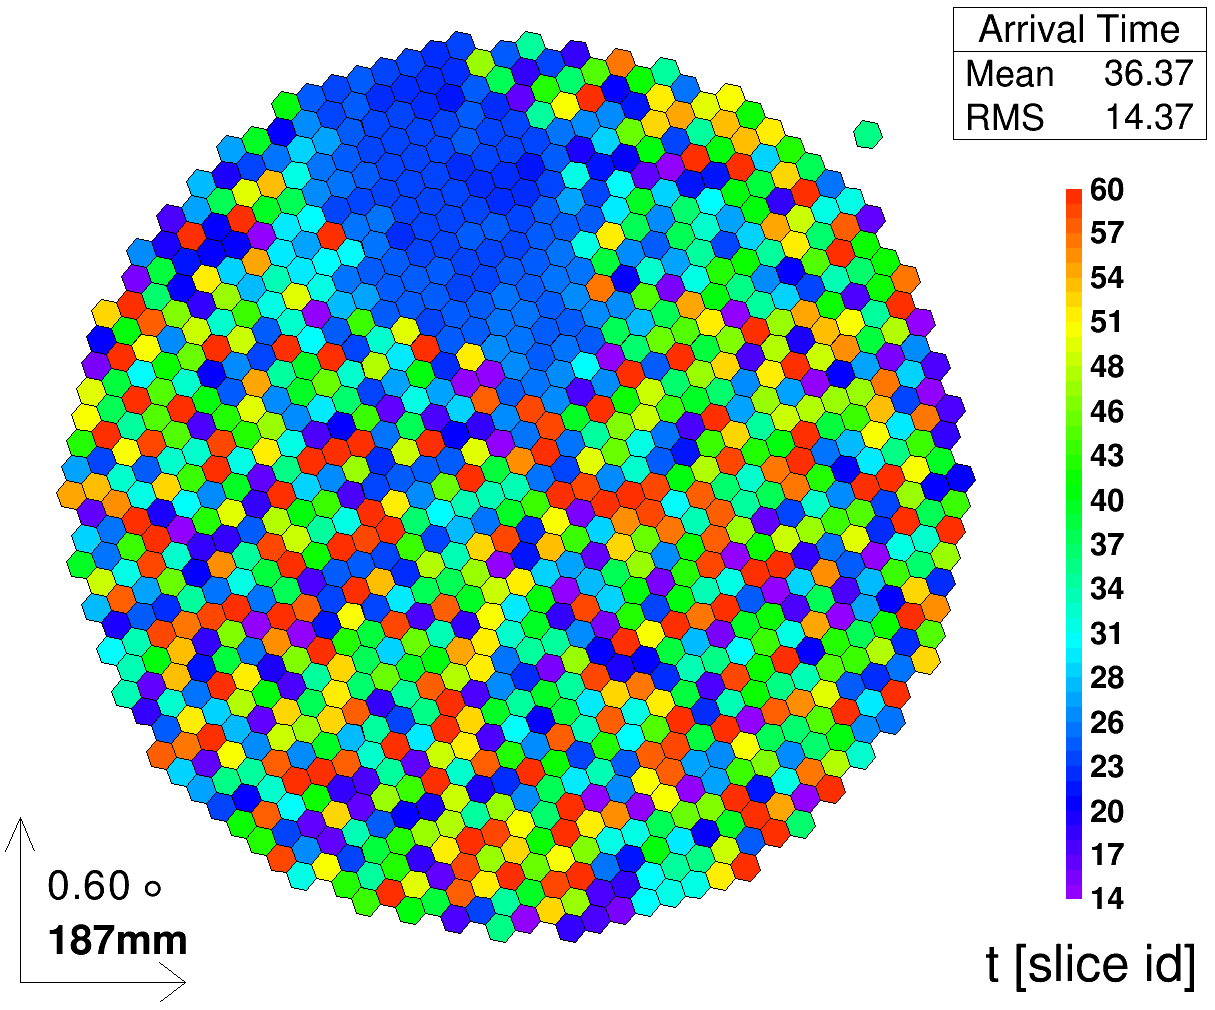
\includegraphics[width=0.6\textwidth]{./Plots/03_MonteCarlos/Signal_ArrivalTime_fertig.png}
    \caption{Darstellung der Ankunftszeiten eines Schauers in der Kamera. Dargestellt sind die Ankunftszeiten in time slices.}
    \label{Kamera-Bild-ArrivalTimes}
\end{figure}

\section{Star - Image Cleaning und Bildparametrisierung}
\label{sec:Star-ImageCleaning}

\subsection{Image Cleaning}
Im Programm \textit{Star} geschieht das Image Cleaning und die Parametrisierung des Schauerbildes.

Wird ein Event getriggert, werden die Signale der einzelnen Pixel gespeichert.
Sowohl Night Sky Background (NSB) als auch elektrisches Rauschen sind dann noch in dem Eventbild enthalten (siehe Abb.\ref{Kamera-Bild}).
Ziel des Image Cleanings ist es, das Bild von allem Background zu bereinigen, sodass nur noch das Signal vom eigentlichen Schauer überbleibt und eine robuste und stabile Parametrisierung dieses Schauerbildes durchgeführt werden kann.
Einerseits können Pixel, die nicht zum eigentlichen Schauer gehören und das Image Cleaning überleben, zu einer falschen Rekonstruktion führen, andererseits ist es zu vermeiden, dass zu viele Pixel im Cleaning wegfallen, da es so zu einem Signalverlust kommt, was ebenfalls zu einer schlechteren Rekonstruktion führen kann.
Also werden schlaue Algorithmen benötigt! 

Der einfachste und älteste Algorithmus ist das Absolute Image Cleaning.
Dabei wird nur die Photoncharge in den einzelnen Pixeln benutzt.
Es werden zwei Schwellwerte definiert für die Core ($Q_{Core}$) und die Boundary Pixel ($Q_{boundary}$).
Nun werden alle Pixel mit einer Photoncharge die größer als $Q_{Core}$ ist, ausgewählt.
Ein Pixel ist dann ein Corepixel, wenn er noch einen Nachbarn hat, welcher ebenfalls eine Photoncharge hat, die dieses Limit überschreitet.
Im zweiten Schritt werden alle Pixel mit direkten Nachbarn, die den vorherigen Schritt überlebt haben und eine Ladung größer als $Q_{boundary}$ haben, als boundary Pixel markiert.
Alle anderen Pixel fliegen raus.
Dieser Image Cleaning Algorithmus benutzt keine Zeitinformation und es wird damit keine niedrige Energieschwelle erreicht. 
Die verschiedenen Rauschlevel zwischen den Pixeln werden auch nicht berücksichtigt.

Eine Weiterentwicklung dieses Cleaningalgorithmus, welcher auch die Zeitinformationen benutzt, ist das Time Constrained Absolute Image Cleaning. 
Es funktioniert genauso wie das absolute Image Cleaning, allerdings wird die Ankunftszeit der Photonen zusätzlich berücksichtigt.

Eine weitere Entwicklung ist das Sum Image Cleaning, welches folgendermaßen funktioniert:
Es wird eine Zweier-, Dreier- oder Vierer-Kombination von Nachbarpixeln gesucht und deren Signale aufsummiert.
Ist das aufsummierte Signal über einer bestimmten Schwelle, werden die Ankunftszeiten in der Gruppe untereinander verglichen. 
Liegen diese nahe genug zusammen, werden die Pixel behalten, ansonsten verworfen.
Anschließend werden Nachbarpixel gesucht und deren Pixelinhalte und Ankunftszeiten betrachtet.

Beim dynamischen Sum Cleaning wird zusätzlich noch die Size, der Gesamtphotoneninhalt, eines Events mit berücksichtigt.

\subsection{Bildparametrisierung}
Die Bildparameter basieren auf den Hillas Parametern von 1985 [] und berücksichtigen die Verteilung der Photonen in den Pixeln, die zum gecleanten Event gehören.
Abb.\ref{Kamera-Bild-gecleant} zeigt ein gecleantes Event in der Kamera.

\begin{figure}
    \centering
    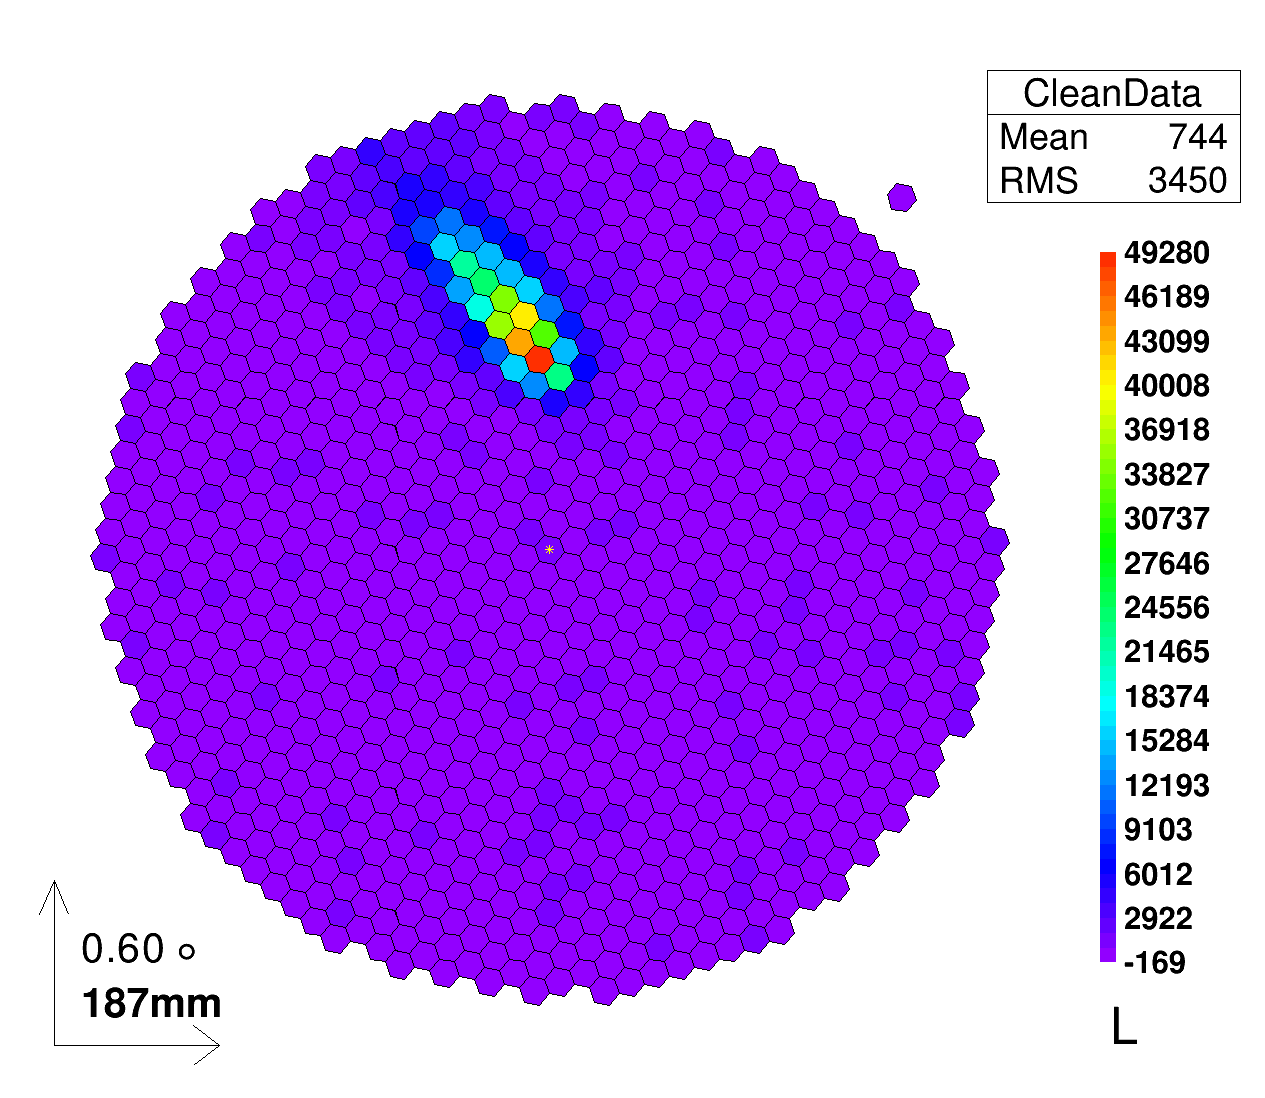
\includegraphics[width=0.6\textwidth]{./Plots/03_MonteCarlos/Signal_gecleant_fertig.png}
    \caption{Darstellung des gecleanten Events in der Kamera.}
    \label{Kamera-Bild-gecleant}
\end{figure}


Im Folgenden werden einige wichtige Bildparameter aufgelistet und beschrieben (vgl. Abb.\ref{CleaningBild}):

\begin{itemize}
 \item \texttt{size}: Die Gesamtzahl der Photoelektronen in einem ShowerImage wird als \texttt{size} bezeichnet. Für feste Zenitwinkel und Impactparameter ist diese Größe proportional zur gesuchten Primärteilchenenergie.
 \item \texttt{CoG} (Center of Gravity): Das Center of Gravity des Schauers bezeichnet die Position des gewichteten Mean Signals entlang der X- und Y-Achse in der Kamera. 
 X und Y sind die ersten Momente der Ladungsverteilung und werden \texttt{MeanX}, bzw. \texttt{MeanY} genannt.
 \item \texttt{Width}: Die halbe Breite der kleinen Halbachse der an den Schauer gefitteten Ellipse wird als \texttt{Width} bezeichnet. 
 Mit Hilfe dieses Paramters lassen sich Aussagen über die transversale Ausbreitung des Schauers und damit auch über den Ursprung des Schauers (hadronisch oder elektromagnetisch) treffen. 
 Dieser Parameter ist somit ein guter Trennparameter.
 \item \texttt{Length}: Die halbe Länge der großen Halbachse wird mit dem Parameter \texttt{Length} bezeichnet.
 Dieser Parameter trifft eine Aussage über die longitudinale Entwicklung des Schauers und ist im Allgemeinen größer für Hadroninduzierte Schauer als für Gammainduzierte Schauer.
 \item \texttt{Conc-n}: Der Anteil der Photoelektronen, welche in den n hellsten Pixeln enthalten sind, wird als \texttt{Conc-n} bezeichnet.
 Damit ist es möglich, die Kompaktheit des Schauermaximums zu beschreiben. 
 Bei Gamma-Schauern ist die Region sehr kompakt.
 \item \texttt{Leakage}: Dieser Parameter beschreibt den Anteil des Signals im äußeren Kameraring im Vergleich zur totalen Image Size.
 Es ist möglich mit diesem Parameter den Signalverlust zu beschreiben und zu entscheiden, ob der Schauer überhaupt noch vernünftig rekonstruiert werden kann.
 \item \texttt{M3Long}: Dieser Parameter ist das dritte Moment entlang der großen Halbachse und beschreibt die Asymmetrie des Schauers.
 Es lässt sich damit also auf die Herkunftsrichtung des Schauers schließen. 
 \texttt{M3Long} ist positiv wenn der Schauerschwerpunkt in Richtung des Kamerazentrums liegt, ansonsten negativ.
 \item \texttt{Number\_of\_Islands}: Wie der Name schon sagt wird mit diesem Parameter die Anzahl der Inseln, die nach dem Cleaning übergeblieben sind, bezeichnet. 
 Je größer dieser Wert ist, umso mehr Inseln sind noch vorhanden und umso wahrscheinlicher ist der Schauer hadronischen Ursprungs.
\end{itemize}

\begin{figure}
    \centering
    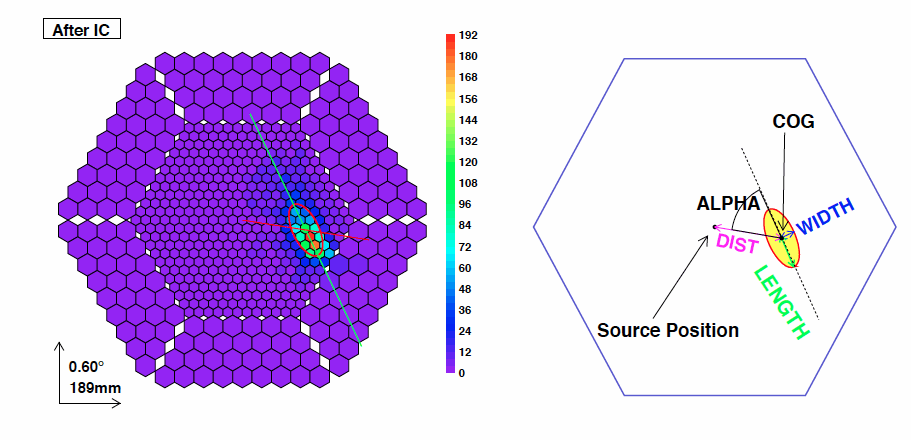
\includegraphics[width=0.9\textwidth]{./Plots/03_MonteCarlos/CleaningBild.png}
    \caption{Beispielhafte Darstellung eines bereinigten Bildes und einiger Bildparameter in der alten MAGIC-Kamera.}
    \label{CleaningBild}
\end{figure}

Abgesehen von diesen Bildparametern gibt es auch noch Parameter, die zu einem bestimmten Referenzpunkt, z.B. der Quellposition, in der Kamera berechnet werden. 

\begin{itemize}
 \item \texttt{Alpha}: \texttt{Alpha} bezeichnet den Winkel zwischen der großen Halbachse der Ellipse und der Linie vom CoG zum Referenzpunkt.
 Dieser Parameter beinhaltet eine große Gamma-Hadron-Trennkraft, da gamma-induzierte Schauer zur Quellposition in der Kamera zeigen und somit alpha klein ist.
 Hadroninduzierte Schauer sind isotrop in der Kamera verteilt.
 \item \texttt{Dist}: \texttt{Dist} ist der Abstand vom CoG zum Referenzpunkt und bietet Informationen über den Abstand von Schauermaximum zur Teleskopachse.
\end{itemize}

Außerdem gibt es noch einige Parameter, die die Ankunftszeit der Cherenkovphotonen zusätzlich berücksichtigen, wie z.B.:

\begin{itemize}
 \item \texttt{TimeGradient}: Der \texttt{TimeGradient} bietet ein Zeitprofil eines Events.
 Die Pixel werden auf die Hauptachse projiziert.
 Dann wird ein Graph der Ankunftszeiten der einzelnen Pixel erstellt und mit einer linearen Funktion gefittet.
 Die Steigung dieser gefitteten Geraden wird dann als Time Gradient bezeichnet.
 \item \texttt{TimeRMS}: So wird der Arrivaltime Spread der Cherenkovphotonen in den Bildpixeln bezeichnet:
 
\begin{equation}
 Time-RMS=\sqrt{\sum_{i=1}^k (t_i-t_{mean})^2}
\end{equation}
 \begin{centering}
  \tiny{mit k:Anzahl der Pixel, $t_i$: Ankunftszeit im i-ten Pixel und $t_mean$:mittlere Ankunftszeit}
 \end{centering}


\end{itemize}

Mit Hilfe dieser Bildparameter und der stereoskopischen Bildparameter kann dann im Folgenden die Gamma-Hadron-Separation durchgeführt werden.


\section{Superstar - Stereoskopische Rekonstruktion der Schauer}
Mit Hilfe des Programms Superstar geschieht die stereoskopische Rekonstruktion der Schauerparameter.

Der Kreuzungspunkt der beiden Hauptachsen der projizierten Bilder des Schauers in den beiden MAGIC-Kameras erlaubt einen Rückschluss auf die Ursprungsrichtung des Schauers.
Anhand geometrischer Überlegungen können die Schauerachse und der Core Impact Punkt auf der Erde, sowie die beiden individuellen Impactparameter der Teleskope bestimmt werden (siehe Abb.\ref{Superstar}).

Auch die Höhe des Schauermaximums wird in Superstar bestimmt.

\begin{figure}
    \centering
    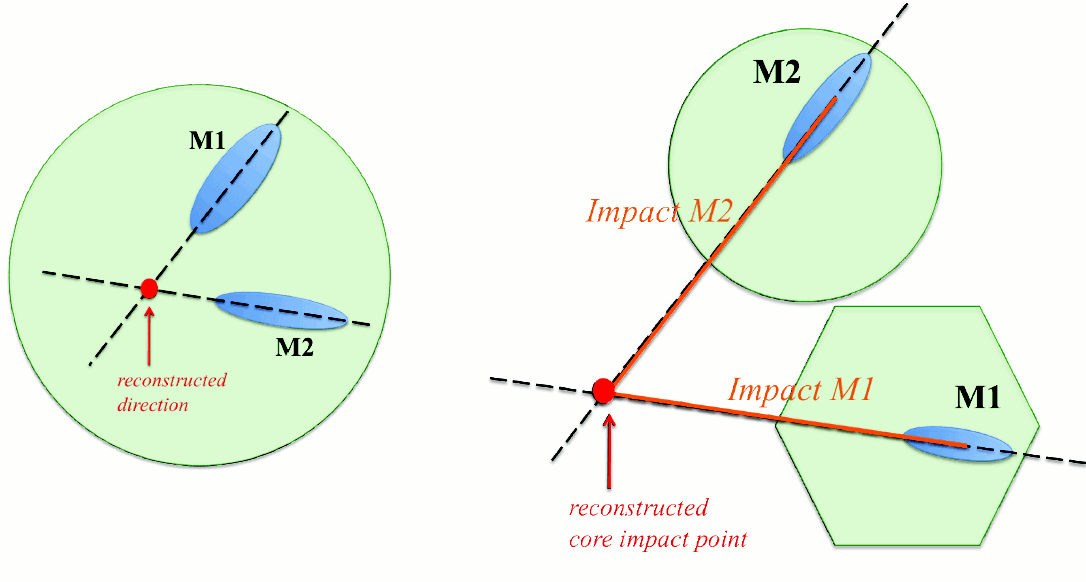
\includegraphics[width=0.9\textwidth]{./Plots/03_MonteCarlos/Superstar.png}
    \caption{Rekonstruierte Richtung und rekonstruierter Core Impact Punkt}
    \label{Superstar}
\end{figure}

Des Weiteren werden noch der Cherenkov-Radius und die Cherenkovlichtdichte bestimmt.

Der Cherenkovradius ist der Radius am Boden, der von einem 87MeV Elektron,welches in Schauerrichtung fliegt, in der Höhe des Schauermaximums produziert wird.

Die Cherenkovlichtdichte ist die Lichtdichte am Boden, die von einem 1m langen Track eines 86MeV Elektrons im Schauermaximum produziert wird, welches ebenfalls in Schauerrichtung fliegt.

%Alle mit Superstar geometrisch berechneten Parameter werden im root Container MStereoPar gespeichert:

% \begin{itemize}
%  \item fCoreX / fCoreY: berechnete CorePosition auf dem Boden
%  \item fDirectionAz/fDirectionDec/fDirectionRA: berechneter Azimut, bzw. Deklination und Rektaszension der Schauerachse
%  \item fM1Impact: berechneter Impactparameter für MAGIC 1, bzw. 2
%  \item fMaxHeight: berechnete Höhe des Schauermaximums
% \end{itemize}

% \begin{figure}
%     \centering
%     
\includegraphics[width=0.9\textwidth]{./Plots/Superstar.jpg}
%     \caption{Stereokacke.}
%     \label{Jobmanager}
% \end{figure}



\section{Automatische MC-Produktion hier in Dortmund geht so}
\label{sec:Automatische MC-Produktion}

Die Monte Carlo Produktion an der TU Dortmund geschieht automatisiert mit Hilfe von bash-Skripten und einer mysql-Datenbank siehe \ref{Jobmanager}.

\begin{figure}
    \centering
    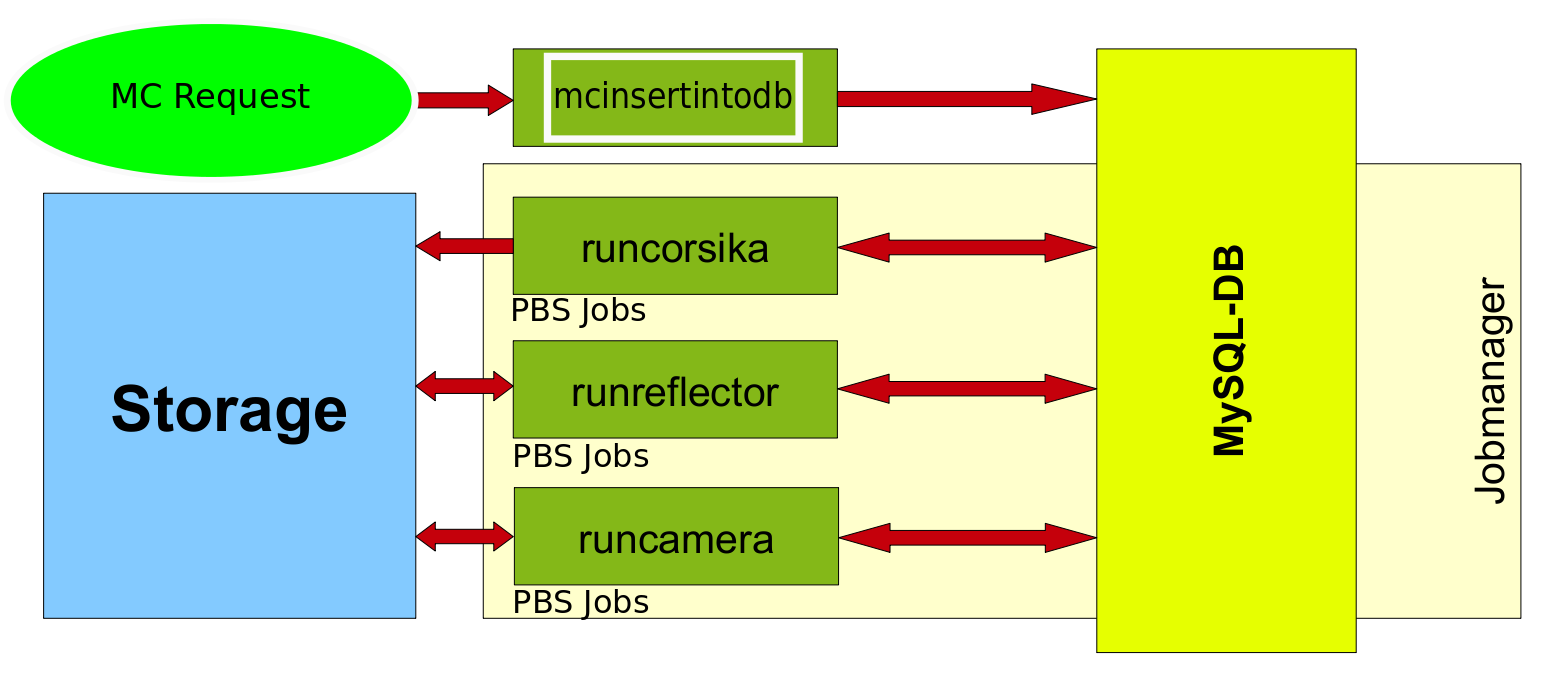
\includegraphics[width=0.9\textwidth]{./Plots/03_MonteCarlos/Jobmanager.png}
    \caption{Schematische Darstellung der automatischen MC Produktionskette.}
    \label{Jobmanager}
\end{figure}


Bei einer neuen Anfrage für MC Daten werden mit Hilfe des mcinsertintodb-Skripts die für die gewünschte Produktion benötigten Inputcard-Parameter in die Datenbank geschrieben.
Im Hintergrund läuft die ganze Zeit das jobmanager-Skript, welches überprüft, ob in der Datenbank ein neuer Auftrag (Job) eingegangen sind.
Falls dies der Fall ist, startet das jobmanager-Skript automatisch das runcorsika-Skript, welches wiederum Corsika für diesen neuen Job mit den gewählten Einstellungen startet.
Sobald Corsika beendet ist, wird dies in die Datenbank geschrieben, sodass das nächste Programm in der Monte Carlo-Kette gestartet werden kann.
Für das nächste Programm in der Kette sind alle benötigten Parameter schon bei der Inauftraggabe des Jobs in der Datenbank gespeichert worden.
Also wird Reflector mit Hilfe des runreflector-Skripts gestartet und nach Beendigung und Eintragen in die Datenbank auch Camera.

Nach dem erfolgreichen Durchlauf eines kompletten Jobs  bestehend aus 1000-2000 Runs mit je 1000 Events werden die generierten MC Daten nach jedem Programmdurchlauf auf dem Cluster gespeichert.
Sobald die Simulationskette für einen Job beendet wurde, wird dies wiederum in die Datenbank eingetragen.

Die Kalibrationskette, die aus den Programmen Sorcerer, Star und Superstar besteht wird analog durchgeführt:
Mit Hilfe der run-Skripte werden die Programme gestartet und nach erfolgreichem Durchlauf die Daten gespeichert.

\subsection{Datenbank}
Wie oben beschrieben, werden die wichtigsten Inputparameter und die Pfade zu den MCs in einer mysql-Datenbank gespeichert.
Diese Datenbank beinhaltet die Tabellen in Tab.\ref{MYSQL_Tabellen}:

\begin{table}[!h]
\centering
\caption{Auflistung der Tabellen, die in der Datenbank existieren....Hmpf!}
\label{MYSQL_Tabellen}
\begin{tabular}{l}
  \toprule
  Tabellen\\
  \midrule
  AtmosphericModel           \\
  AzimuthBinning             \\
  FADCType                   \\
  M1CalibrationProcessStatus \\
  M1CameraCopytoGridStatus   \\
  M1StarCopytoGridStatus     \\
  M2CalibrationProcessStatus \\
  M2CameraCopytoGridStatus   \\
  M2StarCopytoGridStatus     \\
  MCCalibrationRuns          \\
  MCCameraRunData            \\
  MCCorsikaRunData           \\
  MCJobs                     \\
  MCPedestalRuns             \\
  MCReflectorRunData         \\
  MCRunData                  \\
  MCRunProcessStatus         \\
  MCStatistics               \\
  MCSuperstarProcessStatus   \\
  MCUserID                   \\
  MarsVersion                \\
  ObservationMode            \\
  ParticleType               \\
  Source                     \\
  ZenithBinning   	     \\
  \bottomrule
\end{tabular}
\end{table}

% +----------------------------+
% | $Tables_in_magicprod$        |
% +----------------------------+
% | AtmosphericModel           |
% | AzimuthBinning             |
% | FADCType                   |
% | M1CalibrationProcessStatus |
% | M1CameraCopytoGridStatus   |
% | M1StarCopytoGridStatus     |
% | M2CalibrationProcessStatus |
% | M2CameraCopytoGridStatus   |
% | M2StarCopytoGridStatus     |
% | MCCalibrationRuns          |
% | MCCameraRunData            |
% | MCCorsikaRunData           |
% | MCJobs                     |
% | MCPedestalRuns             |
% | MCReflectorRunData         |
% | MCRunData                  |
% | MCRunProcessStatus         |
% | MCStatistics               |
% | MCSuperstarProcessStatus   |
% | MCUserID                   |
% | MarsVersion                |
% | ObservationMode            |
% | ParticleType               |
% | Source                     |
% | ZenithBinning              |
% +----------------------------+

Die Tabelle MCJobs bietet eine Übersicht über alle Jobs. 
Enthalten sind in dieser Tabelle u.a. die JobID, die jedem Job individuell zugewiesen wird, die erste und letzte Runnummer eines Jobs, wann der Job gestartet wurde, wann Camera und Star beendet wurden und den Pfad zu den Daten.\newline
Die Tabellen M1CalibrationProcessStatus und M2CalibrationProcessStatus enthalten ebenfalls die JobID, und die Zeitpunkte wann Camera, Calibration und Star beendet worden. 
Des Weiteren kann man den Startzeitpunkt und den Zeitpunkt eines Abbruchs des Jobs, sowie den zugehörigen Fehlercode sehen, der Rückschlüsse über die Ursache des Fehlers bietet.

In den Tabellen MCCorsikaRunData, MCReflectorRunData und MCCameraRunData kann man die wichtigsten Inputparameter für die jeweiligen Programme sehen.

Die Tabelle MCRunData bietet eine Übersicht über die Runnummern, die innerhalb der einzelnen Programme verteilt wurden. 
So gehört zu jeder Runnumber eine CorsikaRunNumber, eine ReflectorRunNumber und eine CameraRunNumber.
Also bietet ein Job mit 2000 x 1000 Events Platz für 2000 RunNummern pro Programm.

Die Tabelle MCRunProcessStatus ist eine Übersichtstabelle über die Zeitpunkte zu denen die jeweiligen Inputcards geschrieben und die Programme Corsika, Reflector und Camera beendet wurden.

Die gleiche Tabelle gibt es auch noch für Superstar. 


\subsection{LiDO}
Die Monte Carlo-Produktion wird an der TU Dortmund vorwiegend auf dem LiDo-Cluster (Linux Cluster Dortmund) durchgeführt. 
Für die gesamte MAGIC Kollaboration werden hier die Gamma-MCs produziert und gespeichert.

Dafür stehen insgesamt 3328 CPUs und 215TB Speicher auf dem LiDO zur Verfügung.
Die Struktur des Clusters lässt sich Abb.\ref{LiDo} entnehmen.

\begin{figure}[!h]
    \centering
    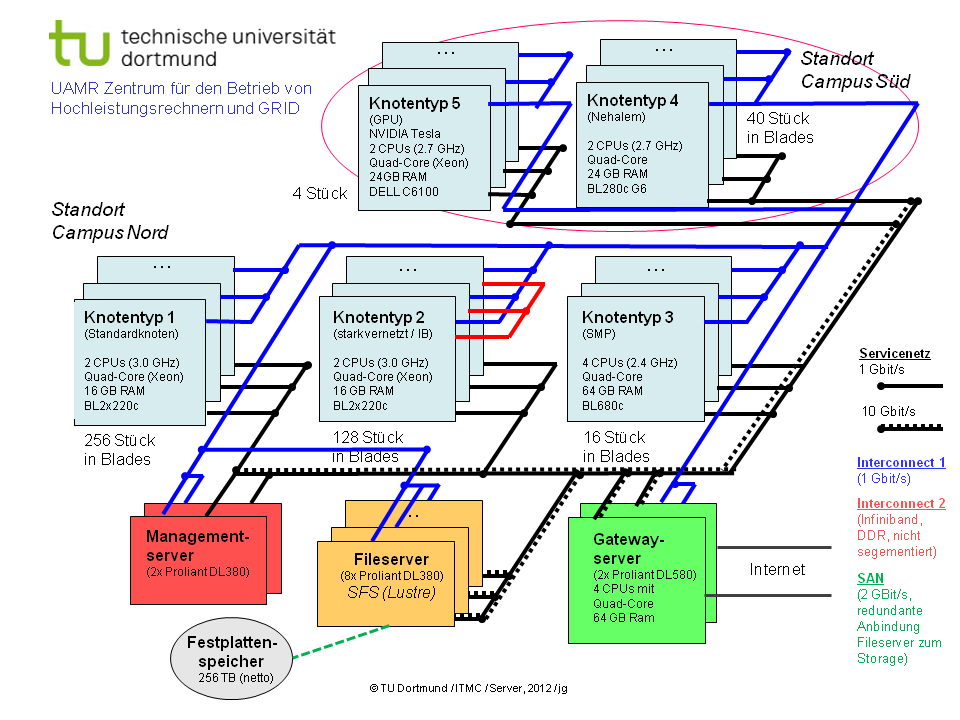
\includegraphics[width=0.9\textwidth]{./Plots/03_MonteCarlos/LiDO.png}
    \caption{Schematische Darstellung des Rechenclusters LiDO.}
    \label{LiDo}
\end{figure}


Über die beiden Gateway-Server erhält man Zugriff auf die Rechenknoten und den Speicher.
Wie in Abb.\ref{LiDo} zu sehen ist, gibt es verschiedene Knotentypen, die sich in der Zahl der maximalen Jobs pro Queue und Nutzer unterscheiden und über ein Queuingsystem erreichbar sind:

\begin{itemize}
 \item Die ib-Knoten sind für parallele Jobs reserviert, die die Infiniband interconnect nutzen
 \item eth-Knoten: Auf diesen Knoten werden serielle und parallele Jobs gerechnet, die die GigabitEthernet Connection nutzen
 \item quad-Knoten: Für Anforderungen an viel Speicher oder parallele OpenMP/Shared Memory Jobs werden die quad Knoten genutzt
 \item GPU: Rechnungen auf Graphikkarten finden hier statt.
 \item nehalem: neue Testknoten mit einer maximaler Walltime von 96h und mehr Arbeitsspecher als die eth-Knoten
\end{itemize}

Die meisten Knoten haben drei verschiedene Queues, die sich in ihrer maximal zur Verfügung stehenden Walltime unterscheiden.
Es gibt als die short Queues (eth, ib, quad) mit einer maximalen Walltime von 1h, die medium Queues (eth, eth\_nhm, ib, quad) mit einer Walltime von 8h und die long Queues mit einer maximalen Walltime von 48h. 
Falls es doch mal länger dauern sollte, gibt es noch die ultralong Queue (eth) mit einer maximalen Walltime von 2688h.
Um also einen Job zu starten, gibt man den benötigten Speicher und eine maximale Walltime an und submittet den Job in das Queuingsystem.

Für die MAGIC MC Produktion werden die eth-Knoten benutzt und pro Run 1000 Corsika Events produziert und weiter prozessiert. 
Ein Standardjob von 2Mio Corsika Events wird also in 2000 Runs mit je 1000 Events darin aufgeteilt und somit 2000 Runs nacheinander an das Queuingsystem submitted.


Im Moment wird auf dem LiDO folgendes Speichervolumen für die Daten nach den verschiedenen Programmen genutzt:

\begin{table}[h!]
    \centering
    \caption{Soviel Speichervolumen wird auf dem LiDo benutzt}
    \label{tab:bsp}
    \begin{tabular}{ccccccc}
        \toprule
        Programm & Corsika & Reflector & Camera & Sorcerer & Star & Superstar\\
        \midrule
        Speichervolumen [TB] & 49 & 36 & 9 & 1.3 & 0.5 & 0.5\\
        \bottomrule
    \end{tabular}
\end{table}

Alternativ kann auch noch der PhiDo Cluster für Testproduktionen, bzw. früher für dezidierte Protonsimulationen benutzt werden. 
Dieser Cluster stellt 1200 CPUs und 200TB(ZAHLEN NACHGUCKEN) Speicher zur Verfügung, hat allerdings auch eine größere Auslastung, was dazu führt, dass eine komplette Produktion wesentlich länger dauert.



\subsection{Wenn die MC fertig sind...Keine Ahnung, ob das interessant ist...}
\label{sec:Wenn die MCs fertig sind}
Sobald eine Produktion an MCs fertig gerechnet ist, werden die Daten ins Grid kopiert.
Das heißt im Moment werden sie auf Computer im Rechenzentrum in Spanien PIC kopiert, welche zum Grid gehören und dort gespeichert, sodass sie immer über eine Internetseite erreichbar sind.
Die Struktur, in der die MCs gespeichert sind, ist so: 

MonteCarlo / Chipsatz der beiden Teloskope / PSF und Mirror fraction / Teilchentyp / Zenitbereich / Observationsart / Standart der Software / Level der Prozessierung / Versionsnummer \newline

\url{http://data.magic.pic.es/Data/MonteCarlo_Stereo/M1_DRS4_1039_M2_DRS4_1039/M1_PSF10.1_MF0.60_M2_PSF8.6_MF0.66/gammas/za05to35/ringwobble/std20140317/superstar/mc_v07/}


%Achten Sie bei ihren Plots auf ausreichend große Achsenbschriftungen, ausreichende Schriftdicken und gut unterscheidbare Farben.
% Im Idealfall haben Sie im Plot und der Arbeit die gleiche Schriftgröße und Schriftart.
% Dies lässt sich durch Erstellen des Plots in der korrekten Größe und einbinden mit dem optionalen Argument \texttt{scale=1} erreichen. Ein Beispiel sehen Sie in Abbildung \ref{fig:bsp}.

% Nutzen Sie wenn möglich Vektorgrafiken (pdf) und nur in Ausnahmen Rastergrafiken wie .png oder .jpg.
% Setzen Sie Punkte hinter Abbildungsunterschriften.
% 
% \begin{figure}[!h]
%     \centering
%     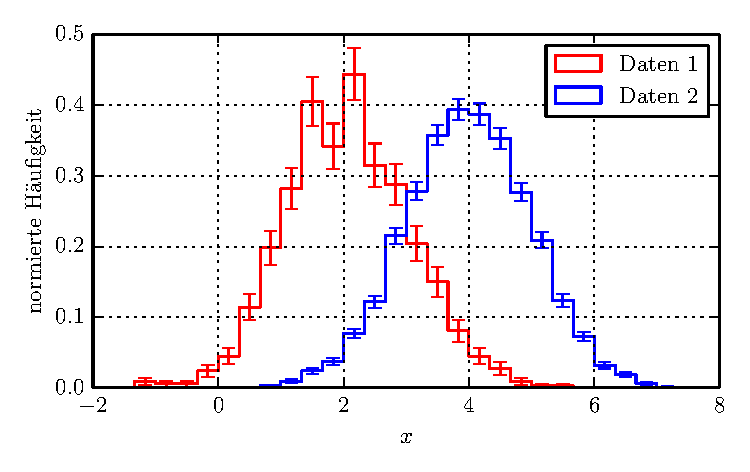
\includegraphics[scale=1]{./Plots/Histogramm.pdf}
%     \caption{Ein Histogramm mit Fehlerbalken für zwei Datensätze, Schriftgröße und -art entsprechen der des Dokuments.}
%     \label{fig:bsp}
% \end{figure}
% 
% \section{Tabellen}
% 
% Tabellen sollten so einfach wie möglich aufgebaut sein, verzichten Sie auf zu viele Linien. In fast allen Fällen reichen drei horizontale Linien aus, jeweils über und unter der Tabelle und zwischen den Spaltenüberschriften und der eigentlichen Tabelle.
% 
% Das Paket \texttt{booktabs} stellt hierfür die Befehle \verb_\toprule_, \verb_\midrule_ und 
% \verb_\bottomrule_ zur Verfügung.
% Das Paket \texttt{siunitx} stellt eine extrem mächtige neue Spalteneinstellung bereit: \texttt{S}, mit ihr können Zahlen und Einheiten sehr sauber und gut ausgerichtet gesetzt werden.
% 
% Diese Vorlage geht von Tabellenüberschriften aus, möchten Sie dagegen Tabellenunterschriften entfernen Sie das entsprechende optionale Argument für die Dokumentenklasse in der Präambel.
% 
% Eine Beispiel ist Tabelle \ref{tab:bsp}.
% 
% \begin{table}[!h]
%     \centering
%     \caption{Beispieltabelle mit willkürlichen Werten, für die Zahlenwerte wurde die S-Option aus SIunitx verwendet, für die Einheitenspalte die s-Option.}
%     \label{tab:bsp}
%     \begin{tabular}{l S[table-format=3.2] S[table-format=3.2(2)] s}
%         \toprule
%         Variable    & {Theoriewert} & {gemessener Wert} & {Einheit}\\
%         \midrule
%         Druck       & 1,23      & 1,31(5)   & \pascal \\
%         Temperatur  & 273,15    & 273,5(2) & \kelvin \\
%         \bottomrule
%     \end{tabular}
% \end{table}

\chapter{Analyse der AGN Mrk 421 mit \textit{MARS}}
\label{chapter:Analyse}
Sowohl die Programme zur Kalibration und Bildparameterbestimmung als auch die Standard-Analyseprogramme sind im \textit{MARS} (MAGIC Analysis and Reconstruction Software)-Paket enthalten.
Dieses Softwarepaket ist eine Sammlung von ROOT-Skripten und Macros.\cite{MARS}

In den folgenden Kapiteln werden die wichtigsten Programme zur Gamma-Hadron-Separation (\autoref{sec:GH-Separation}), Lichtkurven-Berechnung (\autoref{sec:Lichtkurve}) und Spektrums-Rekonstruktion (\autoref{sec:Unfolding}) kurz erklärt.
Danach wird die Analyse der AGN Mrk~421 durchgeführt (siehe \autoref{Mrk421_Analyse}).
Der Datensatz des gesamten Jahres 2012 wird auf Grund von Änderungen der PSF und Hardwareänderungen in vier Teile geteilt und einzeln analysiert. 
In \autoref{LC_Alles} werden dann alle Ergebnisse zu einer gesamten Lichtkurve zusammengefasst.


\section{Signal-Untergrund-Trennung und Energieschätzung}
\label{sec:GH-Separation}
Im Folgenden wird auf die Methode der Signal-Untergrund-Trennung, die Energieschätzung sowie die Rekonstruktion der Quellposition eingegangen.  
Dabei wird die Methode des Random-Forests, welcher zur Gamma-Hadron-Separation und zur Rekonstruktion der Quellposition genutzt wird, erklärt, sowie die Benutzung von Look-Up-Tabellen, mit denen die Energie eines Ereignisses rekonstruiert wird.


\subsection{Gamma-Hadron-Separation}
Da das Signal-Untergrund-Verhältnis zwischen Gamma-Schauern aus der Quelle und hadronischen Schauern kleiner als 1:1000 ist (sogar für helle Quellen), werden gute Verfahren benötigt, um das Signal vom Untergrund zu trennen.
In der Standard-MAGIC-Analysekette übernehmen die Programme \textit{Coach} und \textit{Melibea} diese Aufgabe. 
Es wird zu diesem Zweck ein Random Forest (RF) genutzt. \cite{RandomForestForMAGIC}
Dieser RF basiert auf einem Ensemble an Entscheidungsbäumen mit zufällig ausgewählten Parametern in ihren Knoten.
Um einen solchen RF zu trainieren, wird ein Trainingsset aus MCs und Untergrunddaten benötigt, von denen die Klassenzugehörigkeit (Signal oder Untergrund) genau bekannt ist.

Jedes Ereignis wird durch die in \autoref{sec:Star-ImageCleaning} beschriebenen Bildparameter charakterisiert.
Im Ausgangsknoten eines jeden Entscheidungsbaumes befindet sich das komplette Sample mit allen Bildparametern.
Dieser Knoten wird dann in zwei Nachfolgeknoten geteilt, indem in einem Bildparameter geschnitten wird.
Bei diesem Splittingprozess werden die  Parameter für den Schnitt zufällig aus einer vorher begrenzten Menge gezogen und der Parameter mit dem minimalen Gini-Index zum Schneiden benutzt.

Mit Hilfe des Gini-Index' kann die Ungleichheit der beiden Verteilungen als Funktion des Schnittes angegeben werden, der gerade angewendet wurde.
Ist der Gini-Index von einem Knoten null, so ist in diesem Knoten nur noch eine Klasse vorhanden.
% So bedeutet ein kleiner Gini-Koeffizient, dass die Verteilungen ähnlich sind und ein großer, dass sie ungleich sind. 

Dieses Schneiden geschieht so lange bis die Anzahl der Ereignisse in einem Knoten zu gering wird, oder in einem Knoten nur noch eine Klasse vertreten ist.
In diesen Endknoten (Terminal Nodes) werden dann die Ereignisse mit einem Label (Gamma oder Hadron) versehen. 
Befindet sich in einem Endknoten noch eine Mischung beider Klassen, wird ein Mittelwert vergeben.
So folgt jedes Ereignis einem Pfad durch die i verschiedenen Bäume und wird von allen klassifiziert.
Danach wird ihm ein finales Label, die Hadroness $h$, zugewiesen:

\begin{equation}
 h(Ereignis)=\frac{ \sum_{i=1} ^{n_{B\ddot{a}ume}} l_i(Ereignis)}{n_{B\ddot{a}ume}}
\end{equation}

Es ist möglich in \textit{Coach} alle Variablen auszuwählen, die zum Training der RFs für die GH-Separation, aber auch für die \texttt{Disp}-Bestimmung sowie zum Bauen der Look-Up-Tables zur Energierekonstruktion benötigt werden.
Bei der GH-Separation sind dies elf verschiedene Variablen wie zum Beispiel \texttt{Width} oder \texttt{Length}.
Des Weiteren ist es möglich, die Anzahl der Bäume auszuwählen, sowie den Zenitbereich, in dem diese trainiert werden sollen.

\subsection{Energierekonstruktion mit Hilfe von Look-Up-Tables}
Die Energie der Primärteilchen ist proportional zur Anzahl der Cherenkovphotonen im Schauer und somit auch zum Parameter \texttt{size}.
Allerdings ist \texttt{size} abhängig vom Zenitwinkel, der Lage des Schauers in der Kamera, dem Impact-Parameter und der Höhe des Schauermaximums.

Beruhend auf dieser Tatsache wird nun eine Tabelle erstellt.
Das MC Trainingsset wird in Bins für jeden Parameter, der für die Energierekonstruktion benutzt werden soll, aufgeteilt.
So wird eine mehrdimensionale Tabelle mit der gemittelten Energie der MC-Ereignisse, die zu jedem Bin gehört, erstellt.
Den realen Daten wird dann anhand ihrer Parameter das passende Energiebin in der Tabelle zugeteilt und so eine geschätzte Energie (\texttt{Estimated Energy}) zugeordnet.

Für Mono-Daten geschieht die Energierekonstruktion im Gegensatz dazu auch mit Hilfe eines RFs.


\subsection{Rekonstruktion der Quellposition}
Ziel ist es, die Herkunft des Primärteilchens zu rekonstruieren. 
Der Abstand zwischen dem Schauerschwerpunkt und der Quellposition auf der Hauptachse in der Kamera wird mit dem Parameter \texttt{Disp} bezeichnet.
Es gibt zwei Möglichkeiten, diesen Parameter zu rekonstruieren: Zum Einen sind dies Ghost Busting-Methoden, die die Asymmetrie des Schauers charakterisieren oder aber ein RF.

Bei den Ghost-Busting-Methoden wird die Asymmetrie zwischen Schaueranfang und Schauerende in der Kamera berücksichtigt.
Mit Hilfe des zeitlichen Verlaufs oder des dritten Moments entlang der Hauptachse wird entschieden, aus welcher Richtung der Schauer kommt.

Wird mit zwei Teleskopen observiert, ist die \texttt{Disp}-Rekonstruktion einfacher.
Wie in Abb.\ref{Disp} zu sehen ist, ist perfektes Ghost-Busting möglich.

\begin{figure}
    \centering
    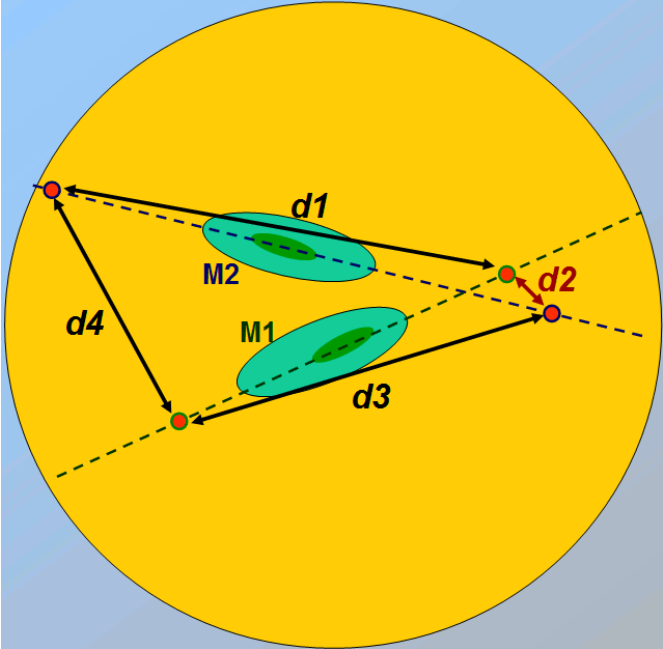
\includegraphics[width=0.5\textwidth]{./Plots/04_MrkAnalyse/Disp.png}
    \caption{Rekonstruktion des Parameters \texttt{Disp}. 
    Wegen der stereoskopischen Beobachtung kann entschieden werden, welche Herkunftsrichtung für den Schauer am wahrscheinlichsten ist.\cite{DispRekonstruktion}}
    \label{Disp}
\end{figure}

Nur eine der beiden möglichen Quellpositionen des einen Teleskops ist kompatibel mit einer der rekonstruierten Quellpositionen des anderen Teleskops. 
Die bevorzugte Position der Quelle ist die, die näher am Schnittpunkt der beiden Hauptachsen liegt und bestimmt \texttt{Disp} für beide Teleskope eindeutig.
Letztendlich wird der gewichtete Mittelwert der beiden wahrscheinlichsten rekonstruierten Quellpositionen genommen.
Ereignisse mit einer zu großen Differenz der beiden rekonstruierten Quellpositionen zueinander werden verworfen.



\section{Berechnung der Lichtkurve}
\label{sec:Lichtkurve}
Der Gammafluss, d.h. die Rate der Gammateilchen $\frac{dN}{dt}$ pro Einheitsfläche, ist Ausgangsgröße für die Lichtkurve:

\begin{equation}
 \Phi=\frac{d^2 N}{dS dt} 
\end{equation}
\begin{centering}
  \small{mit $N$: Anzahl der Teilchen, $S$: Fläche und $t$: Zeit.}
 \end{centering}
 
Dafür wird die Anzahl der detektierten Gammas, die effektive Observationszeit und die effektive Fläche des Detektors benötigt.
Nach der Energie differenziert ist diese Größe der differentielle Fluss pro Energie:

\begin{equation}
 \frac{d\Phi}{dE}=\frac{d^3N}{dSdtdE},
\end{equation}

bzw. der integrale Fluss:
\begin{equation}
 \Phi_{E>500GeV}=\int\limits_{\SI{500}{GeV}}^{\infty}\frac{d\Phi}{dE}dE.
\end{equation}


Die zeitliche Entwicklung des integralen Flusses wird als Lichtkurve bezeichnet.
% Das Binning muss dabei so gewählt werden, dass die Statistik in jedem Bin groß genug ist.
% , tageweise oder minutenweise... Je nachdem, ob gerade irgendwas spannendes passiert (Flares oder so).

\paragraph{Anzahl der Signalgammas}
Um die Anzahl der Gammateilchen aus der Quelle zu bestimmen, wird ein $\theta^2$-Histogramm benutzt.
Dies ist ein Histogramm der quadrierten Entfernungen zwischen der rekonstruierten Quellposition und der nominalen Quellposition.
Gammas aus der Quelle haben ein kleineres $\theta$, während der Background eine annähernd isotrope Verteilung liefert. 
Dies ist beispielhaft in \autoref{Crab_Theta2} gezeigt: schwarz ist die Verteilung der Signal-Ereignisse rot ist die Verteilung der Background-Ereignisse und blau die Differenz aus Signal und Background-Ereignissen. 

\begin{figure}
    \centering
    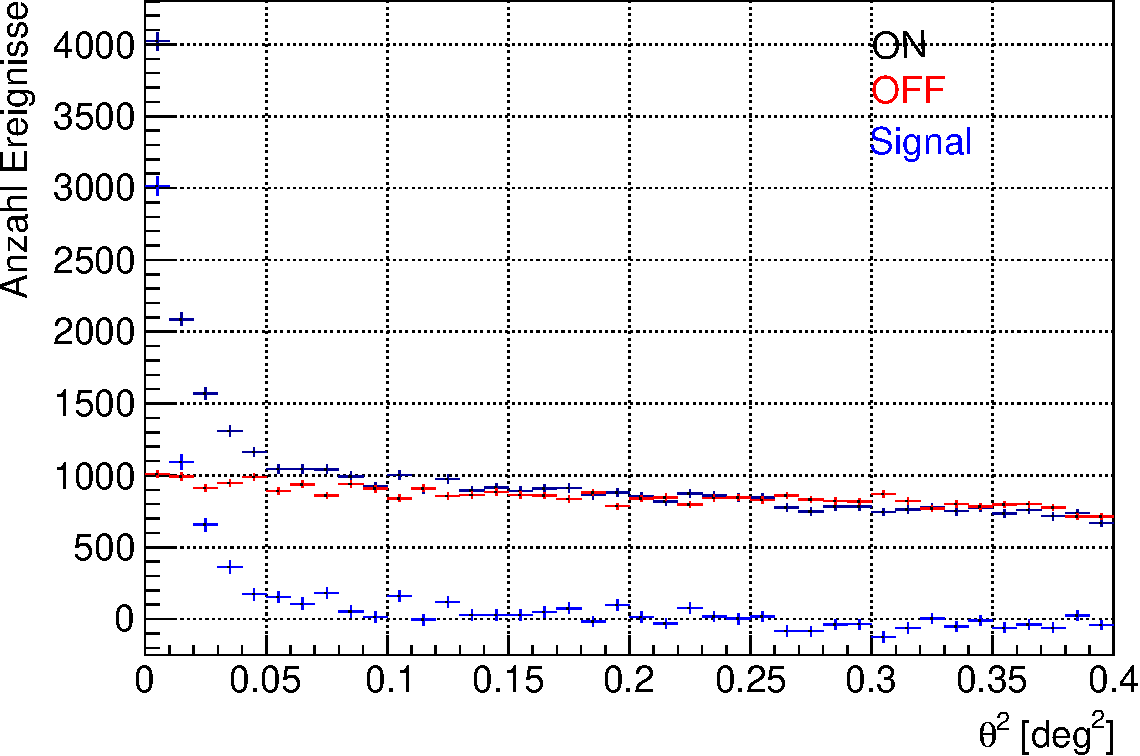
\includegraphics[width=0.8\textwidth]{./Plots/04_MrkAnalyse/Datenset2/Crab_Theta2.pdf}
    \caption{$\theta^2$-Verteilung von Crab-Daten aus dem Datenset 2. 
    Es ist zu sehen, dass die On- (Signal-) und die Background-Daten für $\theta^2 > 0,1$ miteinander übereinstimmen.
    Ereignisse aus der Quelle befinden sich wie erwartet bei $\theta^2 \approx 0$.
    }
    \label{Crab_Theta2}
\end{figure}
% BILDBILDBILD (abelardos talk in zeuthen, der auf der flute seite verlinkt ist)

Um die Anzahl der realen Signal-Ereignisse zu ermitteln, müssen von den Ereignissen aus der Quellrichtung noch die Background Ereignisse abgezogen werden und ein Schnitt in $\theta^2$ angewendet werden.

Dank der ``Wobble-Beobachtung`` ist eine simultane Datennahme von Signal- und Hintergrund möglich, d.h. das Teleskop ist nicht direkt auf die Quelle ausgerichtet, sondern die Quellposition ist $0.4°$ vom Kamerazentrum entfernt.
Wegen der Alt-Azimutalen Montierung rotiert die Quelle um das Zentrum in der Kamera und es ist möglich einen Punkt gegenüber der Quelle als Off-Position zu benutzen.
%Vorteil dieser Methode ist, dass es keine separate Off-Datennahme geben muss.
Es muss gewährleistet werden, dass die Off-Positionen symmetrisch verteilt sind, um Kamerainhomogenitäten entgegenzuwirken.
Allerdings tauchen bei dieser Methode die Quellgammas auch in der Off-$\theta^2$-Verteilung auf, haben aber ein großes $\theta^2$.
Eine Off-Position, die zu nahe an der Quelle ist, ist nicht zu empfehlen.

\paragraph{Effektive Beobachtungszeit}
Die effektive Beobachtungszeit berücksichtigt die Totzeit in der Datennahme.
Nach dem Aufnehmen eines Ereignisses ist die Elektronik mit der Verarbeitung der Daten beschäftigt und neue Ereignisse können nicht detektiert werden.
Die Totzeit ist abhängig vom Chip und beträgt bei den aktuellen DRS4-Chips $\approx 26\mu$s.

\paragraph{Effektive Fläche}
Als effektive Fläche wird die Fläche am Boden bezeichnet, die orthogonal zur Herkunftsrichtung der Schauerteilchen ist.
Die Größe dieser effektiven Fläche ist abhängig von der Energie und dem Zenitwinkel des Schauers.
In \textit{MARS} wird diese Größe mit Hilfe von MCs folgendermaßen berechnet:

\begin{equation}
 A_{eff}(E)=\frac{N_{\gamma, final}}{N_{\gamma, simulated}}A_{MC, total}
\end{equation}

Dafür wird eine bestimmte Anzahl an Gammas ($N_{\gamma, simulated}$) auf einer uniformen Fläche $A_{MC,total}$ simuliert. 
Die Größe $N_{\gamma, final}$ ist die Anzahl der Gammas, die alle Analyseschnitte überlebt hat.


\section{Entfaltung des Energiespektrums}
\label{sec:Unfolding}
Bei der Messung mit IACTs handelt es sich um eine indirekte Messung.
Die Energie des Schauer-auslösenden Teilchens ist nicht direkt messbar.
Die Bildparameter und damit auch die geschätzte Energie $E_{est}$ haben eine begrenzte Auflösung und erfordern die Methode der Entfaltung.

Die Probleme, die bei der Messung auftreten, sind:

\begin{itemize}
 \item Begrenzte Akzeptanz: Nicht alle Schauer, die Teilchen auslösen, können vom Teleskop detektiert werden.
 \item Indirekte Messung: Da eine direkte Messung nicht möglich ist, wird anhand von gemessenen Parametern, wie z.B. der Größe des Schauers in der Kamera, mit Hilfe eines RF die Energie geschätzt.
       Die Vorraussetzung dafür ist, dass diese real gemessenen Parameter stark mit der Energie korrelliert sind.
 \item Begrenzte Auflösung: Es ist nur möglich mit begrenzter Genauigkeit aus den Bildparametern die Energie zu rekonstruieren, d.h. es existiert eine Migration von Ereignissen.
       Wird die geschätzte Energie gegen die reale Energie aufgetragen, erhält man eine verschmierte Diagonale (siehe Abb.\ref{EnergyEst_EnergyTrue})
\end{itemize}

\begin{figure}
    \centering
    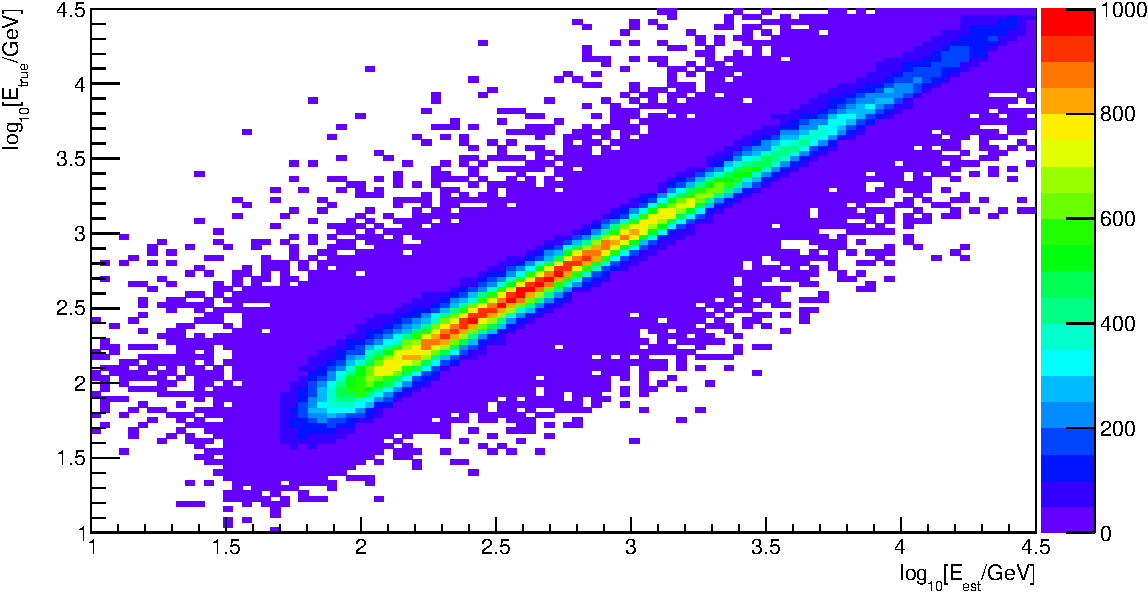
\includegraphics[width=0.8\textwidth]{./Plots/04_MrkAnalyse/EnergyEst_EnergyTrue.pdf}
    \caption{Geschätzte Energie gegen wahre Energie. Es ist erkennbar, dass keine perfekte Energierekonstruktion existiert.}
    \label{EnergyEst_EnergyTrue}
\end{figure}

Durch die Methode der Entfaltung können diese Probleme berücksichtigt werden. 
Das Problem lässt sich mit einer Fredholmschen Integralgleichung darstellen:

\begin{equation}
 g(y)= \int\limits_c^d M(x,y) f(x) dx + b(y)
\end{equation}
\begin{centering}
  \small{mit g(y): gemessene Verteilung, f(x): gesuchte Verteilung, M(x,y): Migrationsmatrix bestimmt auf MCs, b(y): Background-Verteilung}
 \end{centering}

Diese Gleichung lässt sich auch diskretisiert darstellen:

\begin{equation}
 g_i=\sum_j M_{ij}f_j+b_i,
\end{equation}

wobei $M_{ij}$ die Migrationsmatrix ist und damit die Wahrscheinlichkeit beschreibt, dass ein Ereignis in bin $j$ in bin $i$ gezählt wird.

Das Ziel der Entfaltung ist die wahre Verteilung $f$ zu finden.
Die Kovarianzmatrix der gesuchten Verteilung ergibt sich dann mit der Kovarianzmatrix der gemessenen Verteilung zu:

\begin{equation}
 \mathbf{V[\vec{f}]}=\mathbf{M}^{-1}\mathbf{V}[\vec{g}]\mathbf{(M}^{-1})^T.
\end{equation}

Da die Invertierung der Migrationsmatrix oft zu oszillierenden Lösungen führt, wird die Methode der kleinsten Quadrate angewandt.

\begin{equation}
 \chi_0^2=(\vec{g}-\mathbf{M}\vec{f})^T \mathbf{V}^{-1}[\vec{g}](\vec{g}-\mathbf{M}\vec{f}).
\end{equation}

Dies gilt nur für Gauß-verteilte Daten, also nicht für Bins mit kleinen Ereigniszahlen.
Für diese muss nun die Poisson-Statistik benutzt werden und der Log-Likelihood-Ausdruck minimiert werden:

\begin{equation}
 L_0(a)=\sum_i (g_i(a)-g_{i,m}\cdot \ln g_i(a)).
\end{equation}

Außerdem ist es nötig, eine Regularisierung einzuführen, um die kleinen Ausdrücke in der Migrationsmatrix, die während der Entfaltung verstärkt werden, zu unterdrücken.
Durch Einführung eines Regularisierungsterms werden Anforderungen an die Lösung gestellt, bei zu starker Regularisierung aber auch ein Bias eingeführt.

Im Allgemeinen wird Regularisierung durch Addition eines Regularisierungsterms gemacht, sodass:

\begin{equation}
 \chi^2=\chi_0^2 +\frac{\tau}{2} Reg(f).
\end{equation}

Verschiedene Arten der Regularisierung können in der Analyse gewählt werden.
Es ist auch möglich, eine Vorwärtsfaltung durchzuführen, wobei ein bestimmtes Modell als Annahme gewählt wird und freie Parameter dieses Modells bestimmt werden.
Zum Testen ist dies eine gute Alternative, allerdings keine richtige Entfaltung, da das Ergebnis modellabhängig bleibt und physikalische Phänomene verborgen bleiben.

\section{Mrk 421-Analyse}
\label{Mrk421_Analyse}
In diesem Abschnitt wird die Analyse der Daten beschrieben, wobei für jede der vier Datenepochen sowohl die Lichtkurve als auch das Spektrum gezeigt werden.
Dabei wird die Analyse des Datensets 2 der Daten exemplarisch für die Stereo-Analyse erklärt (\autoref{subsec:Datenset_2}), während die anderen Zeitabschnitte des Jahres mit stereoskopischer Beobachtung (\autoref{subsec:Datenset_1} und \autoref{subsec:Datenset_4}) analog ausgewertet werden.
Auf die Mono-Datenanalyse wird in \autoref{subsec:Datenset_3} eingegangen.
Zusammenfassend wird noch eine Lichtkurve aller Daten gezeigt.


\subsection{Überblick über die Daten}
Die Daten, die für diese Analyse zur Verfügung standen, sind Daten der Quelle Mrk~421, die 2012 aufgenommen wurden.
Die Daten gliedern sich folgendermaßen:

\begin{itemize}
 \item Datenset 1: 2012-02-25 - 2012-02-29
 \item Datenset 2: 2012-03-18 - 2012-04-27
 \item Datenset 3: 2012-05-23 - 2012-06-19 (Mono)
 \item Datenset 4: 2012-12-11 - 2012-12-23
\end{itemize}

Datenset 1 und Datenset 2 sind beides Stereobeobachtungen.
Die beiden Datensets unterscheiden sich in ihrer PSF (Point Spread Function), weswegen zwei verschiedene MC-Sets in der Analyse verwendet werden.
Die PSF beschreibt die Abbildungsqualität der Spiegel, bzw. wie gut sie ausgerichtet sind.
Je größer die PSF ist, umso schlechter sind die Abbildungseigenschaften und umso verschmierter ist die Reflexion einer Punktquelle.

Beim 3. Datenset handelt es sich um Mono-Daten. 
Aufgrund der defekten MAGIC-I-Kamera und der geplanten Upgrade-Pause, wurde nur MAGIC-II betrieben.

Im 4. Datenset war das Upgrade abgeschlossen, die alte MAGIC-I-Kamera durch eine neue Kamera ersetzt und es wurden wieder Stereo-Beobachtungen durchgeführt.
Aufgrund der Hardware-Veränderungen und einer anderen PSF wurden wieder neue MCs produziert.

Die Analyse des zweiten Datensets befindet sich in \autoref{subsec:Datenset_2} und die des ersten Datensets in \autoref{subsec:Datenset_1}.
Danach erfolgt die dritte Analyseperiode mit Stereobeobachtungen (Datenset 4) in \autoref{subsec:Datenset_4}.
Die Mono-Analyse wird zuletzt in \autoref{subsec:Datenset_3} beschrieben.


\subsection{Datenset 2}
\label{subsec:Datenset_2}
Anhand der genommenen Mrk 421-Daten, zehn Tage zwischen dem 18.3.2012 (MJD: 56004.1) und dem 27.4.2012 (MJD: 56042.0), wird nun die Stereo-Analyse erklärt.

Diese Daten wurden in einem Zenitwinkelbereich zwischen 12° und 30° genommen (siehe Abb.\ref{Datenset2_fZD}).

\begin{figure}
    \centering
    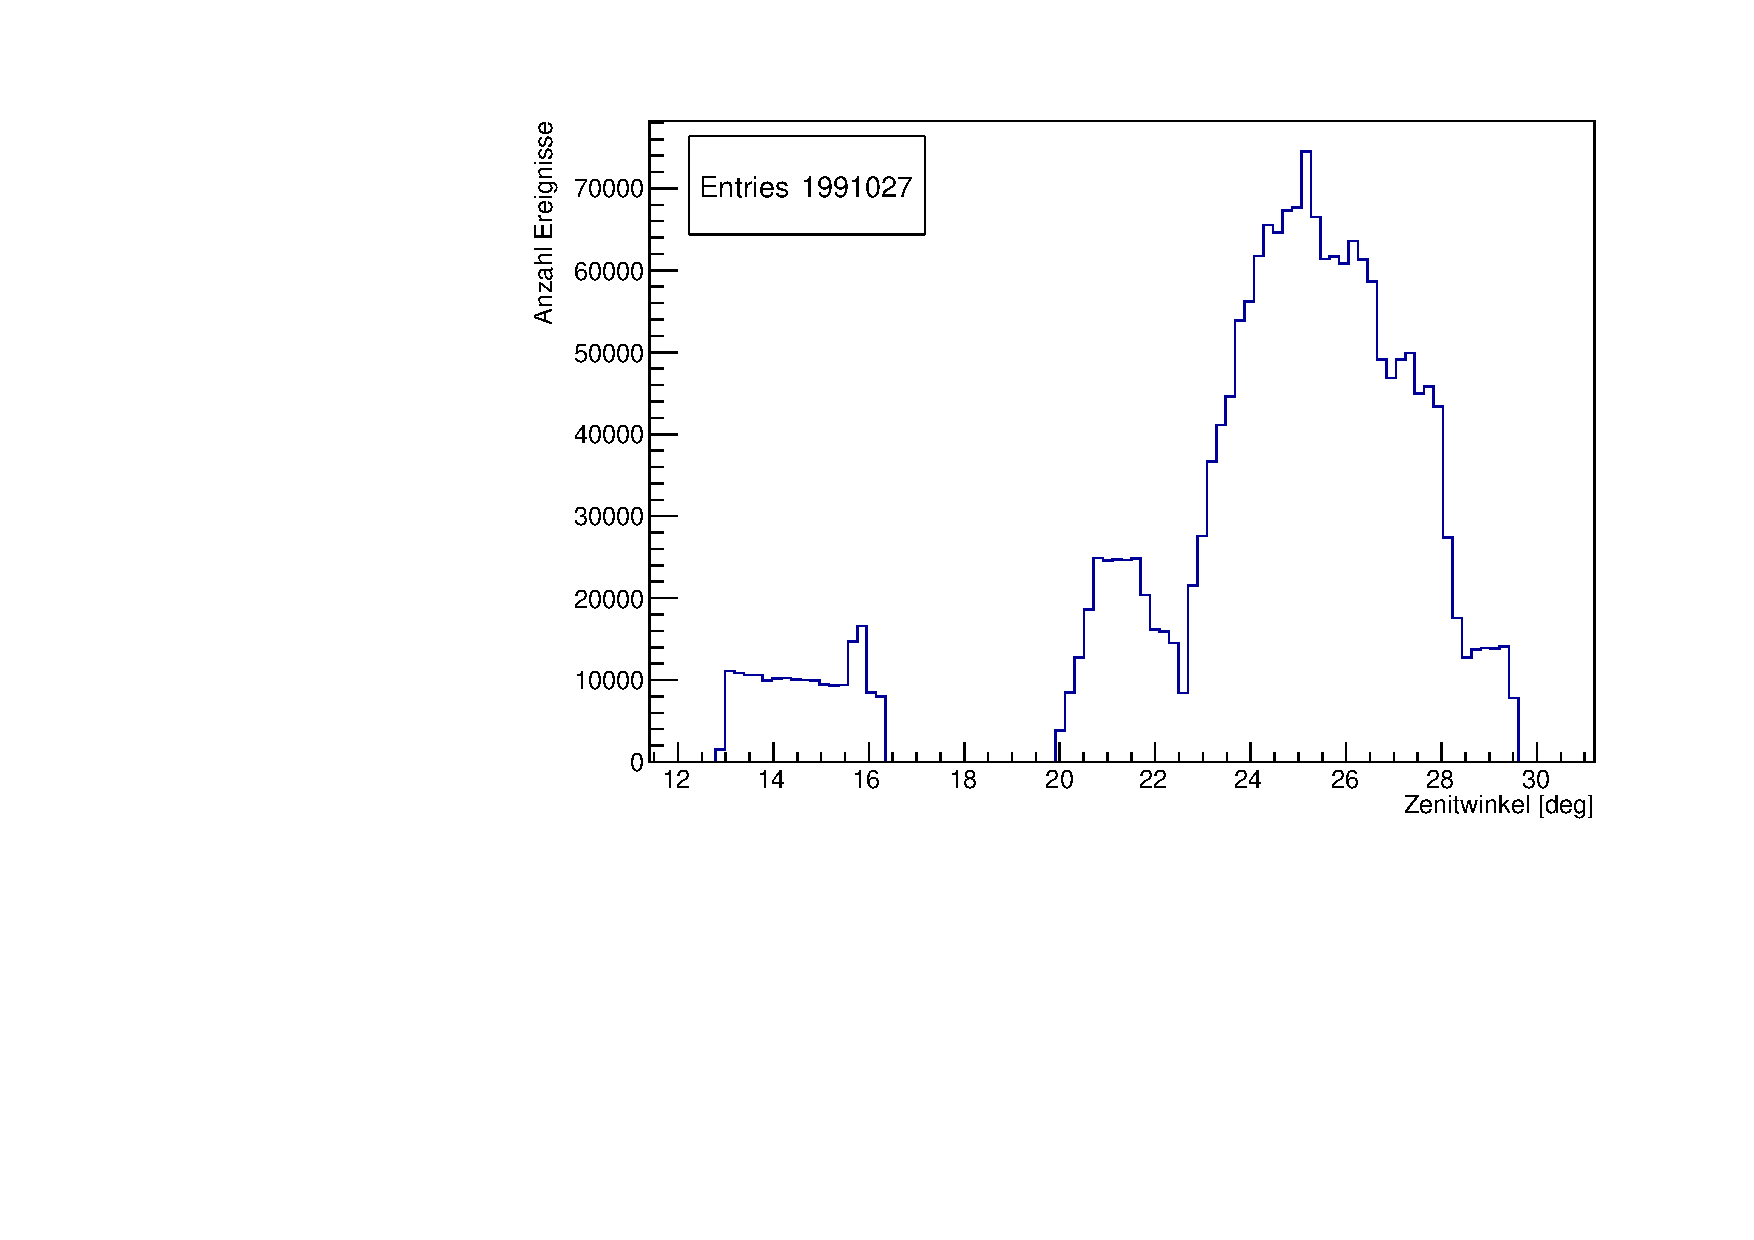
\includegraphics[width=0.7\textwidth]{./Plots/04_MrkAnalyse/Datenset2/Datenset2_Mrk421_MPointingPos_fZd.pdf}
    \caption{Zenitverteilung der genommenen Mrk 421-Daten zwischen dem 18.3.2012 und dem 27.4.2012.}
    \label{Datenset2_fZD}
\end{figure}


Da dieser Datensatz die meisten Daten beinhaltet, wird die Analyse exemplarisch hiermit durchgeführt.

Als Background-Daten dienen Daten anderer Quellen, welche in der gleichen Zeitspanne wie die zu analysierenden Daten liegen.
Dadurch wird gewährleistet, dass das Teleskop die gleichen Eigenschaften, wie z.B. PSF, hat wie bei der Datennahme der zu analysierenden Quelle. 

Mit Hilfe von Crab-Daten werden die Einstellungen für die Lichtkurvenbestimmung bestimmt, da Crab als Standardkerze dient und einen bekannten stabilen Fluss hat. 


\subsubsection{Daten-Auswahl und Qualitätchecks}
Zunächst werden die auf \textit{Superstar}-Level prozessierten Daten einem Datencheck unterzogen, um die Daten herauszufiltern, die bei guten Bedingungen genommen wurden.
Gute Bedingungen sind durch dunkle Nächte, gutes Wetter, wenig Störlicht durch z.B. Autoscheinwerfer und keine Hardware- oder Softwareprobleme gekennzeichnet.

Um dunkle Bedingungen zu gewährleisten wurde zunächst ein Cut im Direct Current (DC) (MAGIC-I < $\SI{500}{nA}$, MAGIC-II < $\SI{800}{nA}$) durchgeführt.
Danach wurden mit Hilfe des \textit{MARS} Macros \textit{Quate} alle Daten mit einem Zenitwinkel < 35° ausgewählt, Runs mit einer Länge unter $\SI{10}{s}$ und Runs mit einer Abweichung des Pointings von 15arcmin verworfen.
Außerdem wurden die Mittelwerte der Rate, der Parameter \texttt{Number of Islands}, \texttt{Concentration}, \texttt{Width} und \texttt{Length} gebildet und ebenfalls Ausreißer aussortiert um eine gute Qualität der Daten zu gewährleisten.

Diese Kriterien für den Datencheck wurden für die Mrk 421-Daten, die Crab-Daten und die Background-Daten angewendet.

In der Tabelle \ref{tab:Datenset2-Mrk421} ist aufgelistet, an welchen Tagen Mrk 421-Daten nach dem Datencheck für die Analyse zur Verfügung stehen.


\begin{table}[!h]
\centering
\caption{Übersicht über alle nach dem Datencheck zur Verfügung stehenden Daten von Mrk~421 aus Datenset 2.}
\label{tab:Datenset2-Mrk421}
\begin{tabular}{ll}
  \toprule
  Monat & Tage\\
  \midrule
  \midrule
März & 18., 22., 28.\\
April & 11., 13., 15., 19., 21., 23., 25. \\
  \bottomrule
\end{tabular}
\end{table}

Tabelle \ref{tab:Datenset2} zeigt wieviele Minuten Daten, Background-Daten und Crab-Daten den Datencheck überstanden haben. 
Auf eine tageweise Auflistung der Background- und Crab-Daten wird verzichtet.

\begin{table}[!h]
\centering
\caption{Übersicht über alle an nach dem Datencheck zur Verfügung stehenden Daten von Mrk~421-, Crab- und Background aus Datenset 2.}
\label{tab:Datenset2}
\begin{tabular}{lc}
  \toprule
  Quelle & Observationszeit [min]\\
  \midrule
  \midrule
  Mrk 421 & 272\\
  \midrule
  Crab & 161\\
  \midrule
  0FGLJ0631 & 77 \\
  1ES1011 & 492 \\
  1ES1426 & 424 \\
  PG1553 & 971 \\
  PKS1222 & 247 \\
  SegueJ & 3252 \\
  \bottomrule
\end{tabular}
\end{table}

Für diesen Teil der Analyse werden die in Dortmund produzierten Standard-MC-Daten im Zenitbereich 5°-35° genommen, in denen die alte MAGIC-I Kamera simuliert wurde.
Die PSF für MAGIC-I beträgt hierbei $\SI{10,5}{mm}$ und die Mirror Fraction 0.58, während diese Werte für MAGIC-II $\SI{10,2}{mm}$ für die PSF und 0.70 für die Mirror Fraction sind.

Es ist zu beachten, dass für alle Daten (Mrk 421/Crab/Background) und die MCs das gleiche Cleaning benutzt wird, da zu dieser Zeit zwei verschiedene Cleaning-Schwellen im Next-Neighbor-Cleaning gebräuchlich waren.
Die Schwellwerte für die Kern und Nachbarpixel betragen in diesen Daten 6, bzw. 3.


\subsubsection{\textit{Coach} und \textit{Melibea}}
Für das Training des RF für die GH-Separation und die \texttt{Disp}-Bestimmung sowie das Erstellen der Look-Up-Tables zur Energierekonstruktion ist es wichtig, dass in jedem Zenitbin ausreichend Background- und MC-Daten vorhanden sind.
Es wird ein Zenitbereich von 10-35° ausgewählt.
Wie in Abb.\ref{Datenset2_Zenitverteilung_Off} und Abb.\ref{Datenset2_Zenitverteilung_MC} zu sehen ist, ist diese Voraussetzung erfüllt.

\begin{figure}
    \centering
    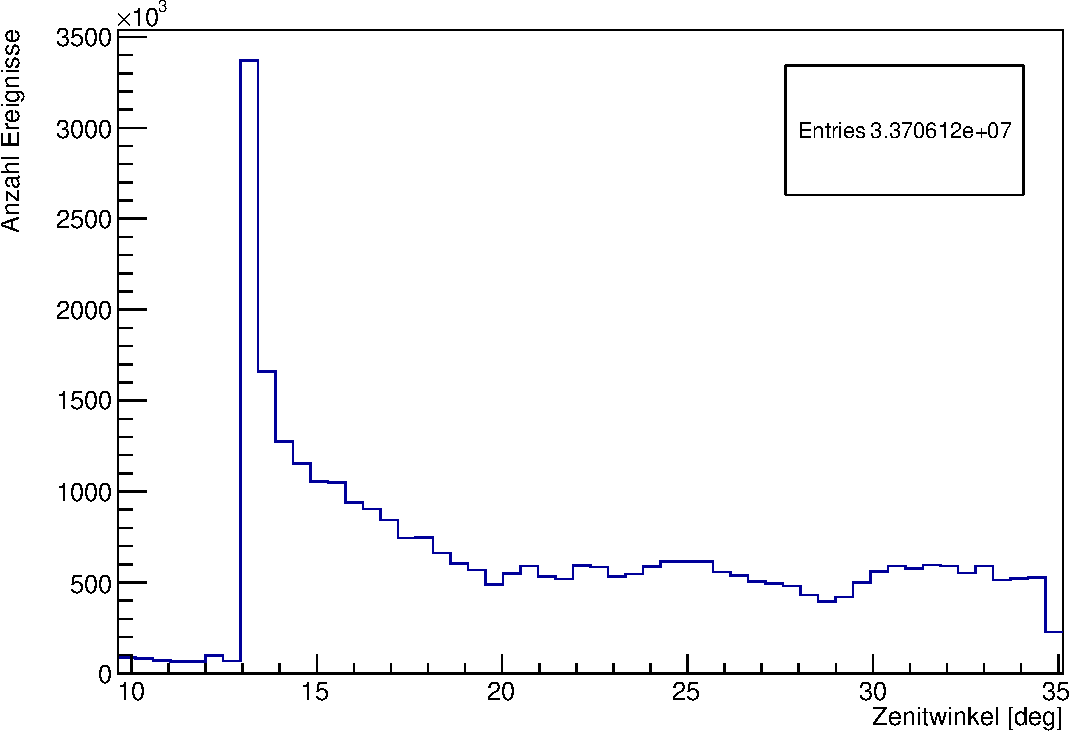
\includegraphics[width=0.7\textwidth]{./Plots/04_MrkAnalyse/Datenset2/Datenset2_Background_MPointingPos1_fZd.pdf}
    \caption{Zenitverteilung der Background-Daten zwischen dem 18.3.2012 und dem 27.4.2012.}
    \label{Datenset2_Zenitverteilung_Off}
\end{figure}

\begin{figure}
    \centering
    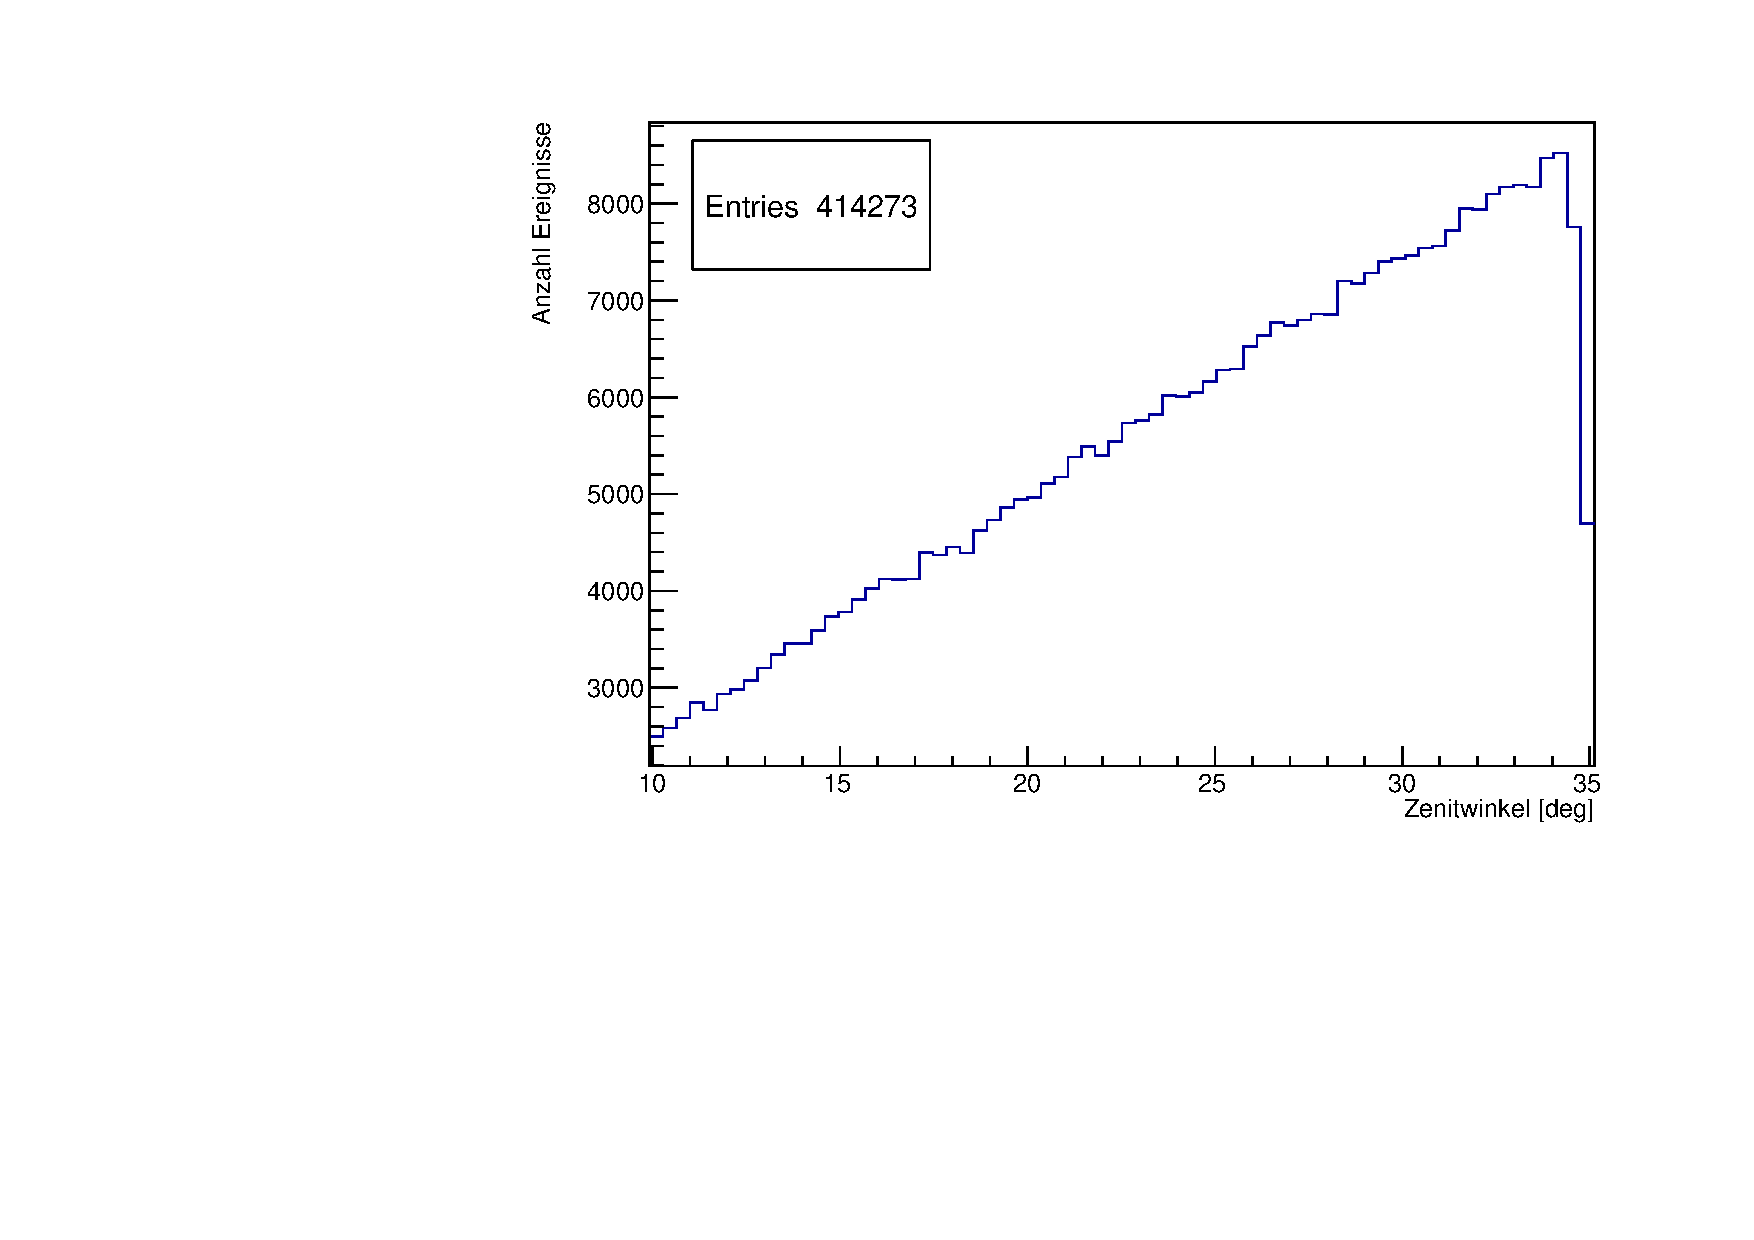
\includegraphics[width=0.7\textwidth]{./Plots/04_MrkAnalyse/Datenset2/Datenset2_MC_MPointingPos1_fZd.pdf}
    \caption{Zenitverteilung des Trainingssets der MC.}
    \label{Datenset2_Zenitverteilung_MC}
\end{figure}

Der MC-Datensatz wurde in zwei Teile geteilt.
Der eine Teil, das Trainings-Set, wird zusammen mit den Background-Daten zum Trainieren des RF für die GH-Separation und für die \texttt{Disp}-Abschätzung benutzt, sowie zum Aufstellen der Look-Up-Tables für die Energie.
Der andere Teil wird später zur Bestimmung der effektiven Fläche zur Entfaltung benutzt.

Sobald das Training der RFs und das Erstellen der Look-Up-Tables in \textit{Coach} beendet ist, werden in \textit{Melibea} die Daten nach Gamma- und Hadron-Ereignis klassifiziert und jedem Ereignis eine geschätzte Energie und ein \texttt{Disp}-Wert zugeordnet.
Das gleiche geschieht auch mit den Crab-Daten und dem anderen Teil der MCs, dem Test-Set.


\subsubsection{Lichtkurve von Crab}
Wie in \autoref{sec:Lichtkurve} beschrieben, wird nun sowohl für die Crab-Daten als auch für die Mrk 421-Daten eine Lichtkurve erstellt.
Da der Fluss von Crab stabil und bekannt ist, werden mit Hilfe der Crab-Daten die passenden Parameter (Hadroneffizienz und $\theta$-Quadrat-Effizienz) für die Lichtkurven-Bestimmung in diesem Zeitraum für Mrk~421 ausgewählt.

Wie in \autoref{Datenset2_Flute_Plots_Crab} zu sehen ist, ist es möglich mit \textit{Flute} neben der Lichtkurve (vgl. Abb.\ref{Datenset2_LC_Crab}) auch noch einen $\theta^2$-Plot (vgl. Abb.\ref{Datenset2_theta^2_Crab}), sowie die spektrale Energieverteilung (vgl. Abb.\ref{Datenset2_SED_Crab}) zu berechnen.

\begin{figure}
  %-----------------------------Figure 1--------------------------------------------------------%
  \begin{subfigure}{0.45\linewidth}
  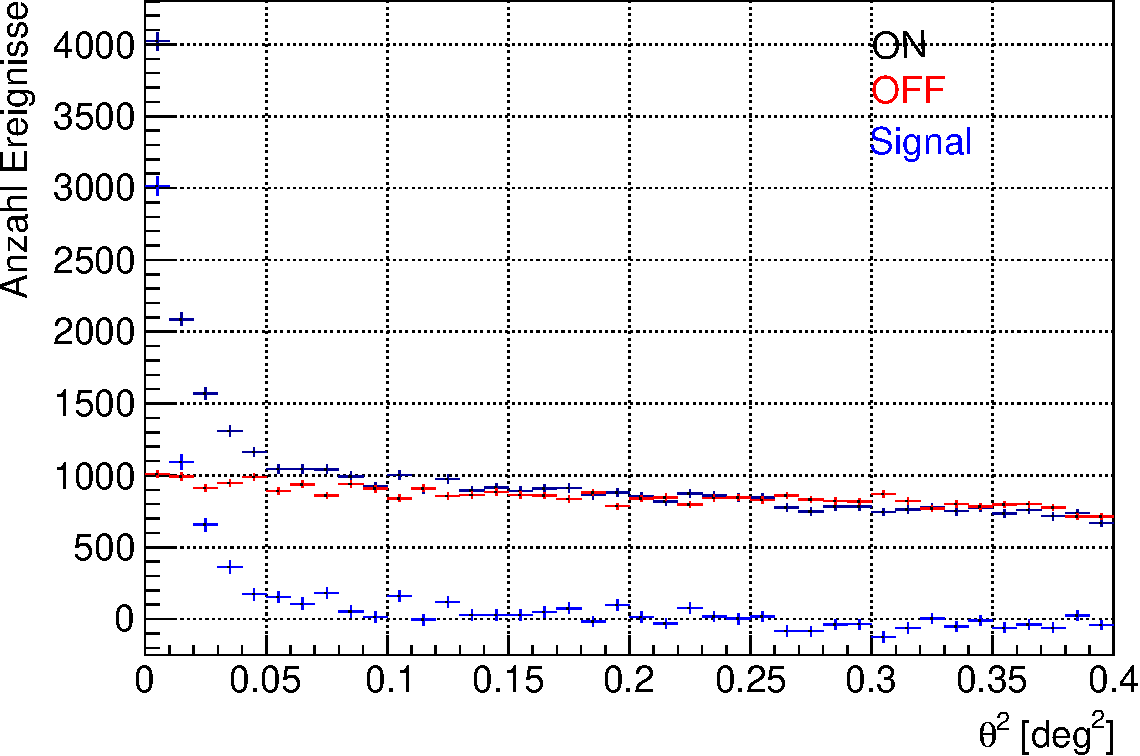
\includegraphics[width=\textwidth]{./Plots/04_MrkAnalyse/Datenset2/Crab_Theta2.pdf}
  \caption{$\theta^2$-Plot für Crab für alle Wobble-Positionen}
  %für den Energiebereich zwischen 5.5 GeV und 55.43TeV
  \label{Datenset2_theta^2_Crab}
  \end{subfigure}
  \hfill
  %-----------------------------Figure 2--------------------------------------------------------%
  \begin{subfigure}{0.45\linewidth}
  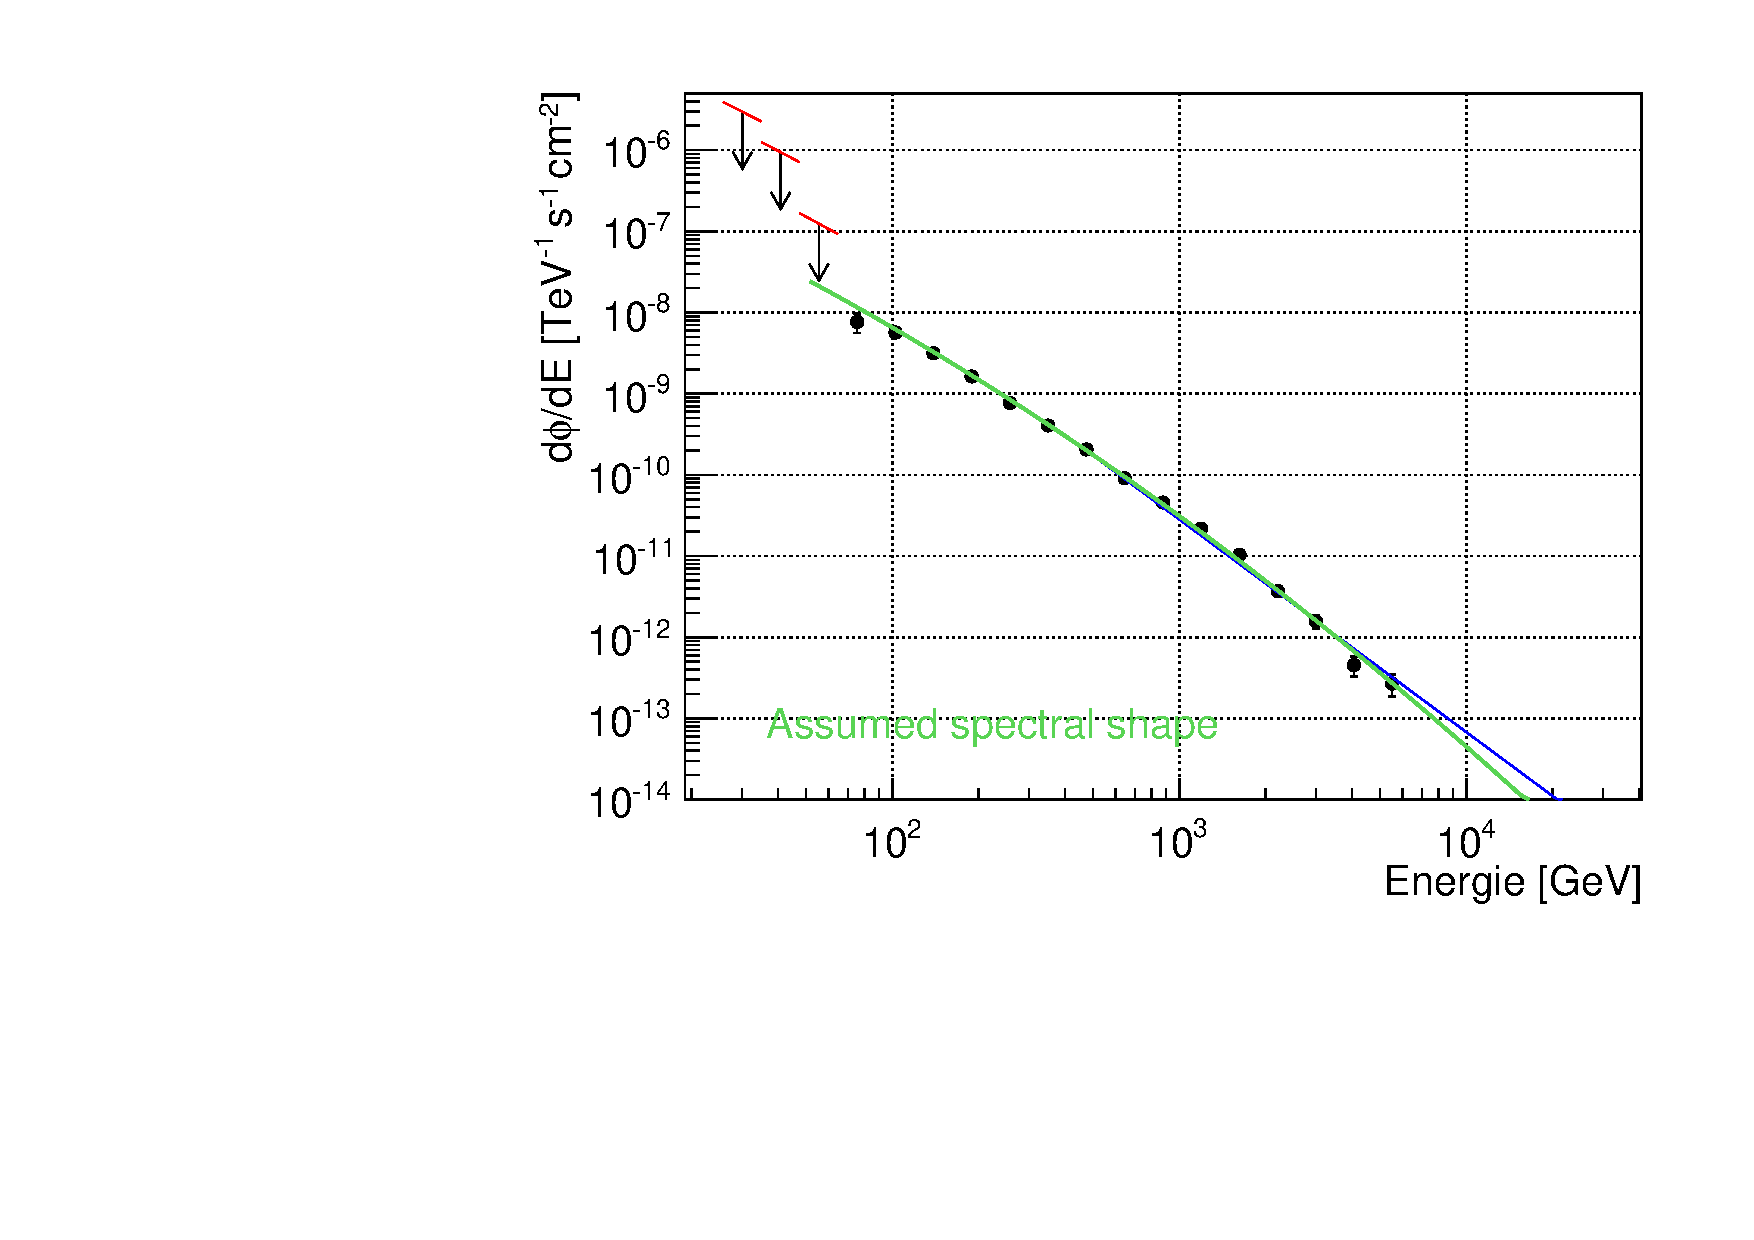
\includegraphics[width=\textwidth]{./Plots/04_MrkAnalyse/Datenset2/Crab_dFdE.pdf}
  \caption{Differentielles Energiespektrum}
  \label{Datenset2_SpectralShape_Crab}
  \end{subfigure}
  \hfill
  %-----------------------------Figure 3--------------------------------------------------------%
  \begin{subfigure}{0.45\linewidth}
  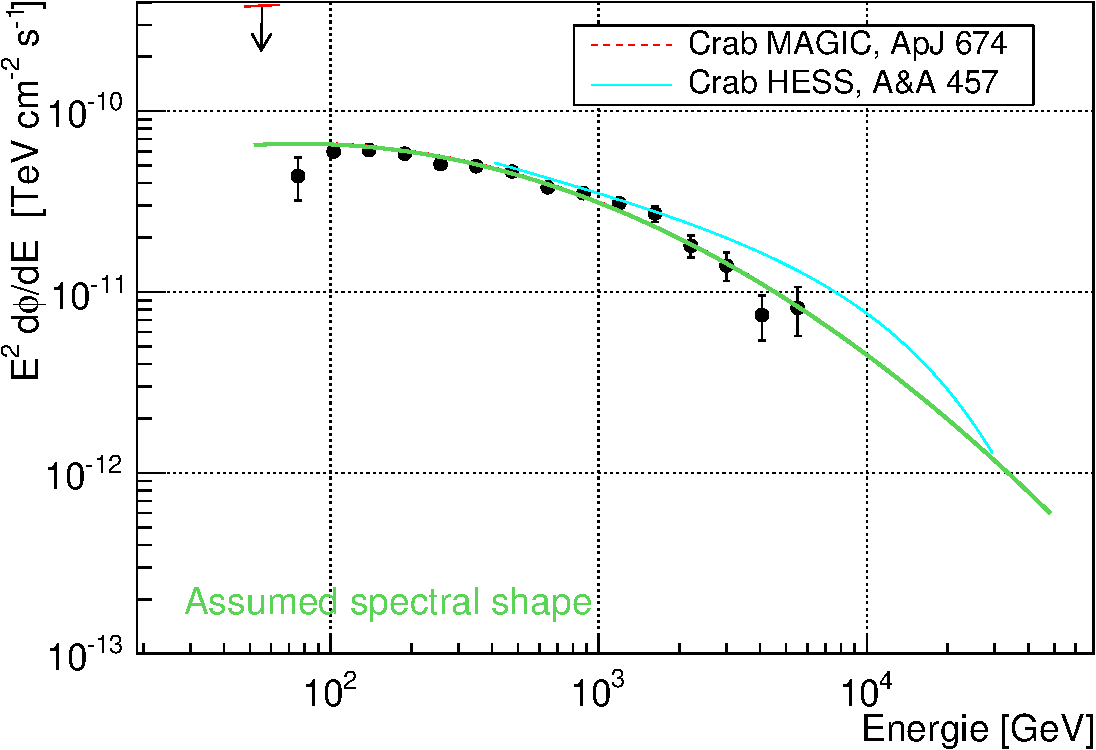
\includegraphics[width=\textwidth]{./Plots/04_MrkAnalyse/Datenset2/Crab_SED.pdf}
  \caption{Spektrale Energieverteilung}
  \label{Datenset2_SED_Crab}
  \end{subfigure}
  \hfill
  %-----------------------------Figure 4--------------------------------------------------------%
  \begin{subfigure}{0.45\linewidth}
  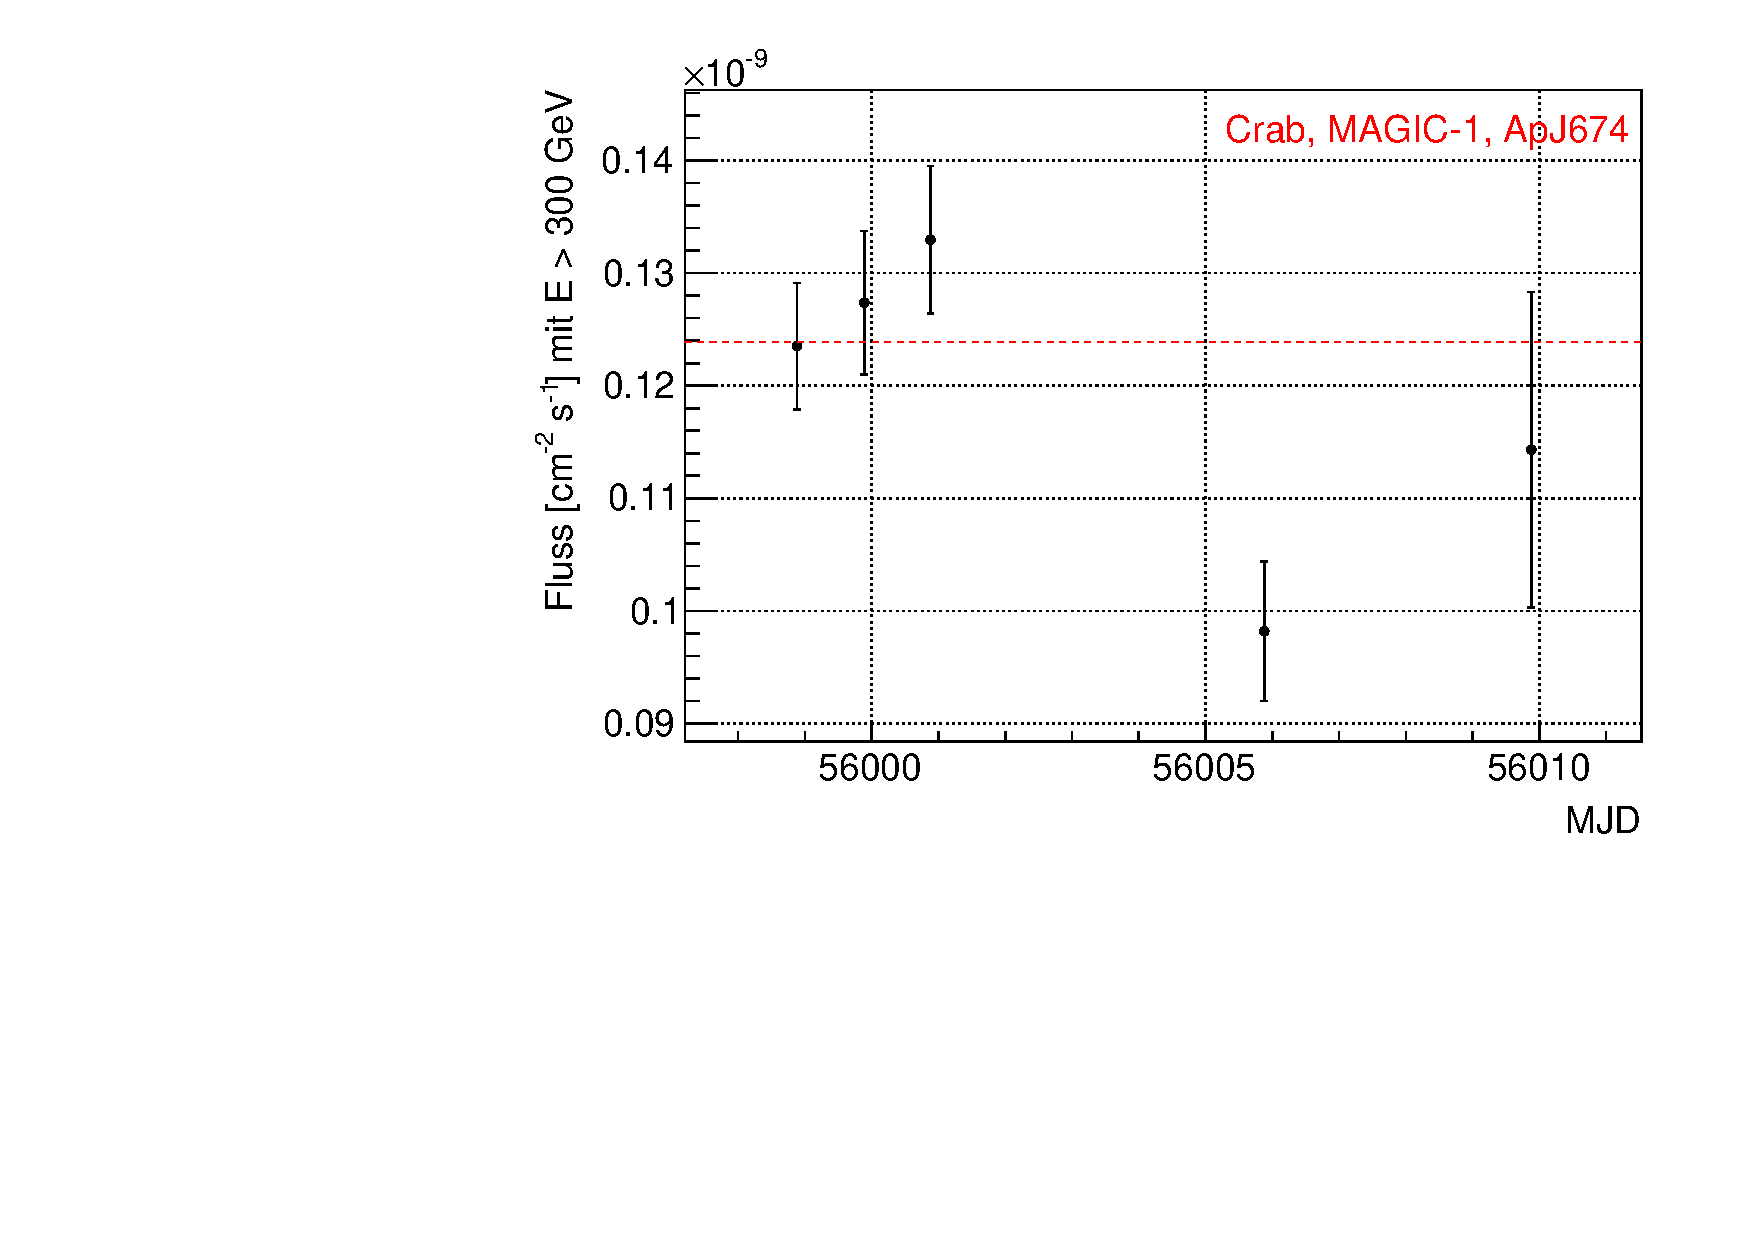
\includegraphics[width=\textwidth]{./Plots/04_MrkAnalyse/Datenset2/Crab_LC.pdf}
  \caption{Lichtkurve von Crab mit mittlerem Fluss von Crab}
  \label{Datenset2_LC_Crab}
  \end{subfigure}
  \hfill
  %----------------------------------------------------------------------------------------------%
\caption{\textit{Flute}-Plots für Crab}
\label{Datenset2_Flute_Plots_Crab}
\end{figure}

In \autoref{Datenset2_theta^2_Crab} ist der $\theta^2$-Plot für Crab zu sehen. Für kleine $\theta$ ist die Anzahl der Signal-Ereignisse wie zu erwarten sehr hoch.

In \autoref{Datenset2_SpectralShape_Crab} ist das differentielle Energiespektrum zu sehen.
In blau ist das von HESS gemessene Spektrum von Crab eingezeichnet.

\autoref{Datenset2_SED_Crab} zeigt die spektrale Energieverteilung, d.h. das mit $E^2$ gewichtete Spektrum aus \autoref{Datenset2_SpectralShape_Crab}.
Das in der Literatur angegebene Spektrum ist durch eine rot gestrichelte Linie gekennzeichnet, die unter dem angenommenen Spektrum, dargestellt als grüne Linie, liegt.
Zum Vergleich ist ebenfalls wieder ein von HESS gemessenes Spektrum eingezeichnet.

Wie in Abb.\ref{Datenset2_SpectralShape_Crab} und in Abb.\ref{Datenset2_SED_Crab} zu sehen ist, passt das angenommene Spektrum gut zu den Daten, bzw. zum bekannten Crab-Spektrum.
Dieses angeonommene Spektrum ist in den beiden Abbildungen durch die grüne Linie gekennzeichnet.
Angenommen wurde:

\begin{equation}
\frac{dN}{dE}=\left(\frac{x}{\SI{300}{GeV}}\right)^{-2.31-0.26\cdot log_{10}(x/\SI{300}{GeV})}\si{TeV\,cm^{-2}\,s^{-1}}.
 %pow(x/300.,-2.31-0.26*log10(x/300.))
\end{equation}

Die Lichtkurve in Abb.\ref{Datenset2_LC_Crab} zeigt, dass der Crab-Fluss in diesem Zeitraum um den mittleren Crab-Fluss schwankt.
Die Parameter, die zum Erstellen der Lichtkurve in \textit{Flute} verwendet wurden, erweisen sich also als vernünftig.

\subsubsection{Lichtkurve von Mrk 421}
Es wird nun mit den gleichen Effizienz-Einstellungen wie für Crab eine Lichtkurve für Mrk 421 angefertigt.

\begin{figure}
    \centering
    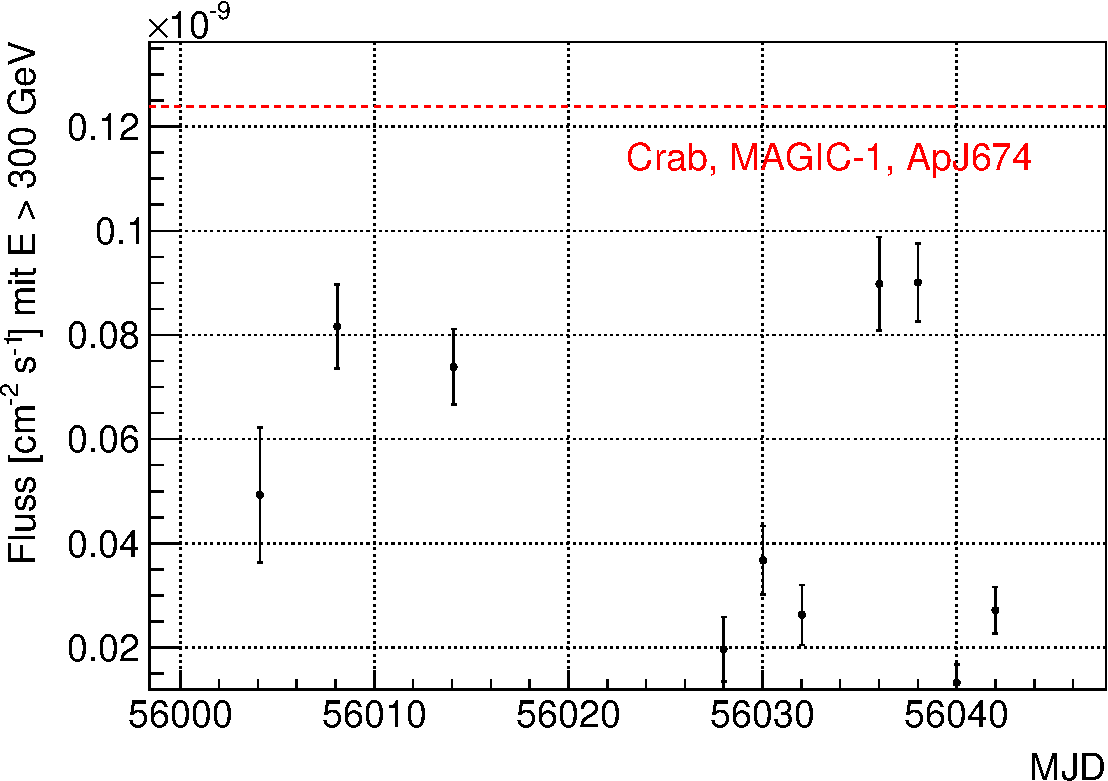
\includegraphics[width=0.8\textwidth]{./Plots/04_MrkAnalyse/Datenset2/LC_Mrk421.pdf}
    \caption{Lichtkurve von Mrk 421 im Zeitraum vom 18.3.2012 bis zum 25.4.2012.}
    \label{Datenset2_LC_Mrk421}
\end{figure}

Abb.\ref{Datenset2_LC_Mrk421} zeigt, dass der Fluss von Mrk 421 im Vergleich zu Crab wesentlich niedriger ist.
Er schwankt etwa um den halben Crab-Fluss.
Auch die spektrale Energieverteilung sieht anders aus (vgl. Abb.\ref{Datenset2_SED_Mrk421}), da ein anderes Spektrum angenommen wurde:

\begin{equation}
\frac{dN}{dE}=\left(\frac{x}{\SI{300}{GeV}}\right)^{-2.75-0.26 \cdot log_{10}(x/\SI{300}{GeV})}\si{TeV\,cm^{-2}\,s^{-1}}
\end{equation}


\begin{figure}
    \centering
    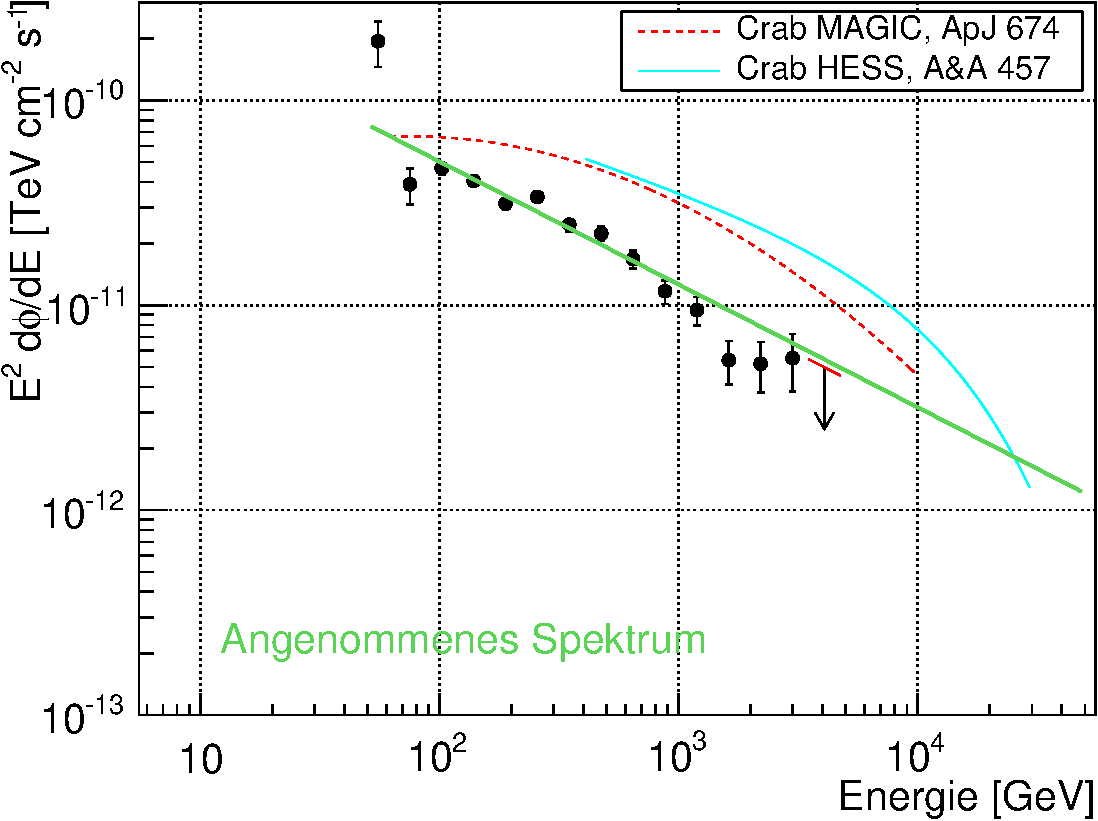
\includegraphics[width=0.8\textwidth]{./Plots/04_MrkAnalyse/Datenset2/SED_Mrk421.pdf}
    \caption{Spektrale Energieverteilung von Mrk 421.}
    \label{Datenset2_SED_Mrk421}
\end{figure}


\subsubsection{Spektrum von Crab}
Mit Hilfe von \textit{CombUnfold} wird nun das Spektrum von Crab entfaltet.
\autoref{Datenset2_CombunFold_Crab} zeigt das entfaltete Spektrum von Crab mit Literaturwert \todo{REFERENZ}.

\begin{figure}
    \centering
    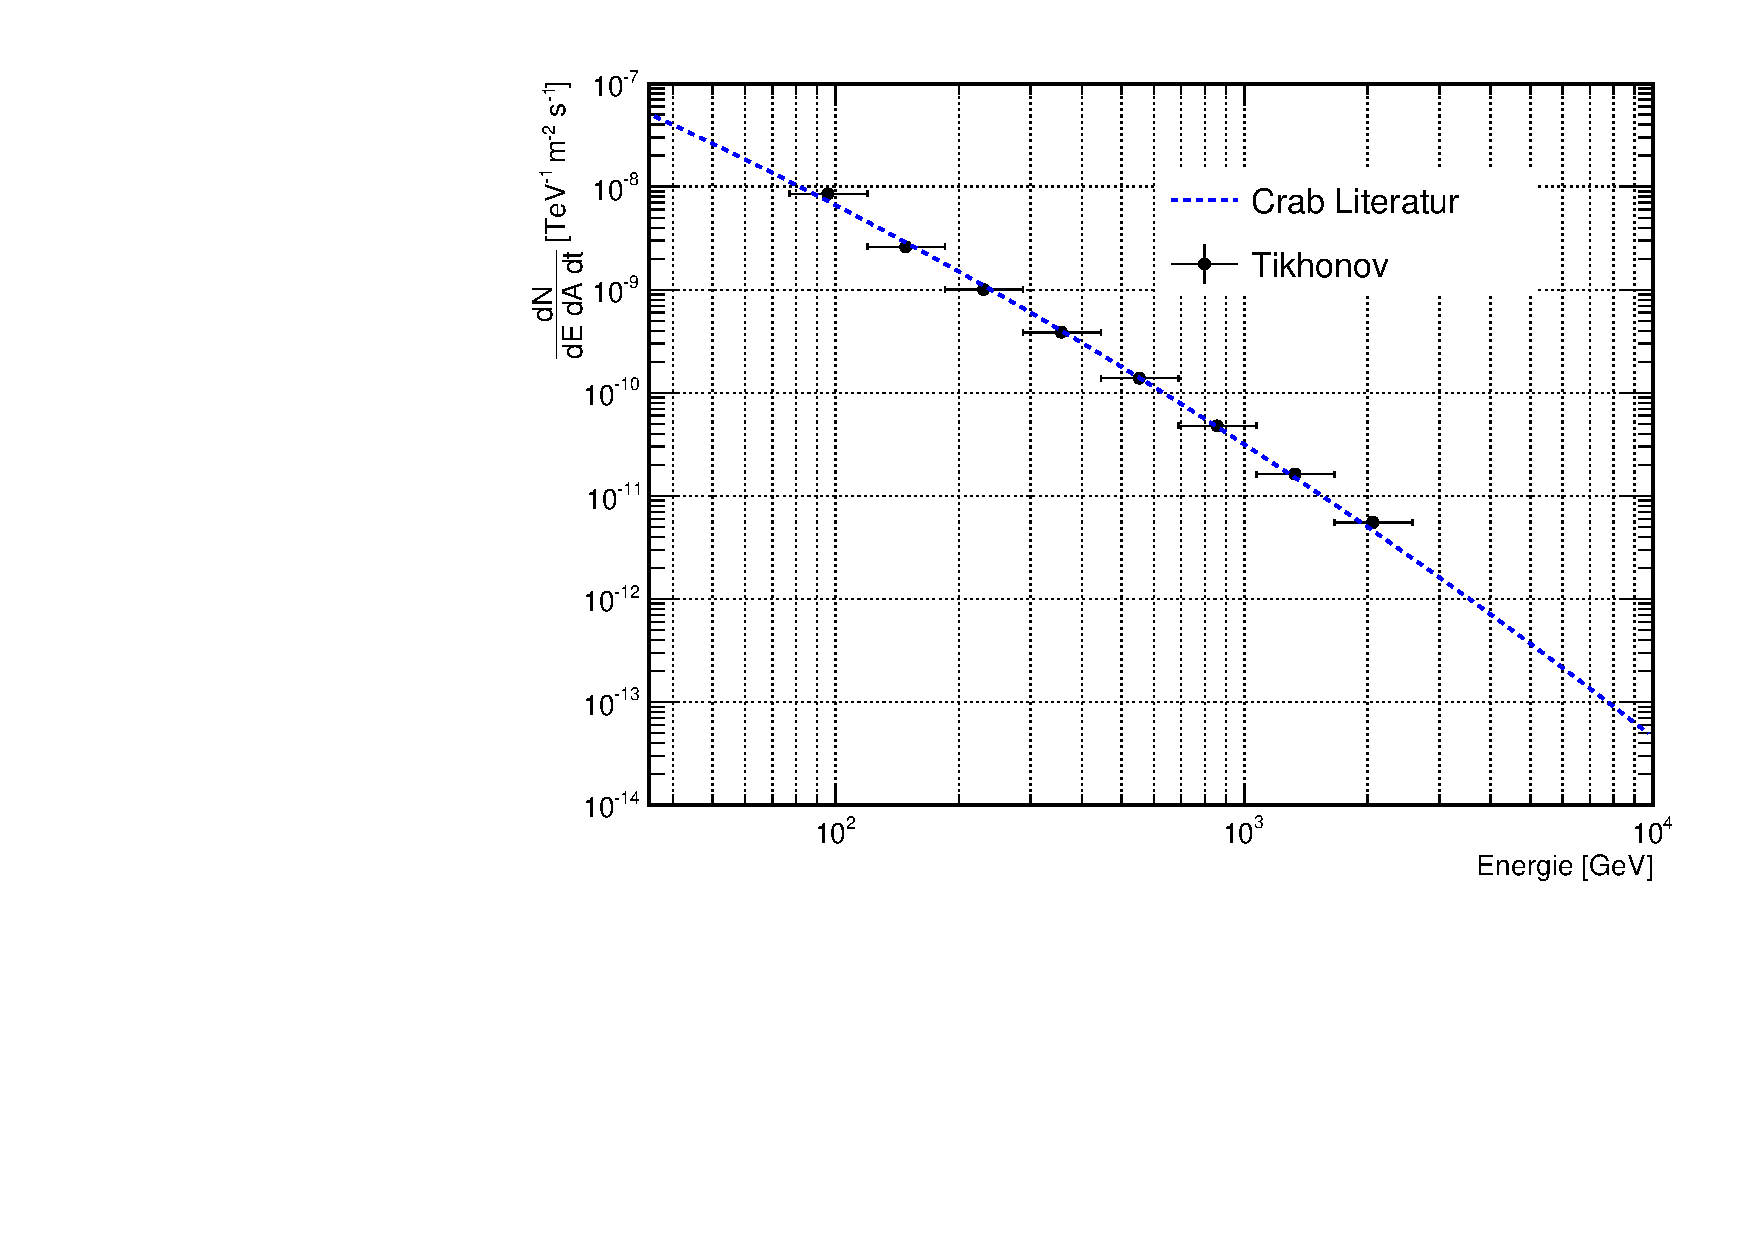
\includegraphics[width=0.8\textwidth]{./Plots/04_MrkAnalyse/Datenset2/Crab_mit_Literatur.pdf}
    \caption{Entfaltetes Crab-Spektrum im Zeitraum vom 18.3.2012 bis zum 25.4.2012 mit Literaturwerten.}
    \label{Datenset2_CombunFold_Crab}
\end{figure}

Es zeigt sich, dass die entfalteten Datenpunkte mit Tikhonov-Regularisierung sehr gut zum Literaturwert passen.

\subsubsection{Spektrum von Mrk 421}
\autoref{Datenset2_CombunFold_Mrk421} zeigt das entfaltete Spektrum von Mrk 421 mit fünf verschiedenen Regularisierungsmethoden.
Wie man sieht, zeigen die entfalteten Datenpunkte keine großen Abweichung voneinander. 
Lediglich bei kleinen Energien unterscheiden sich die Ergebnisse etwas.

\begin{figure}
    \centering
    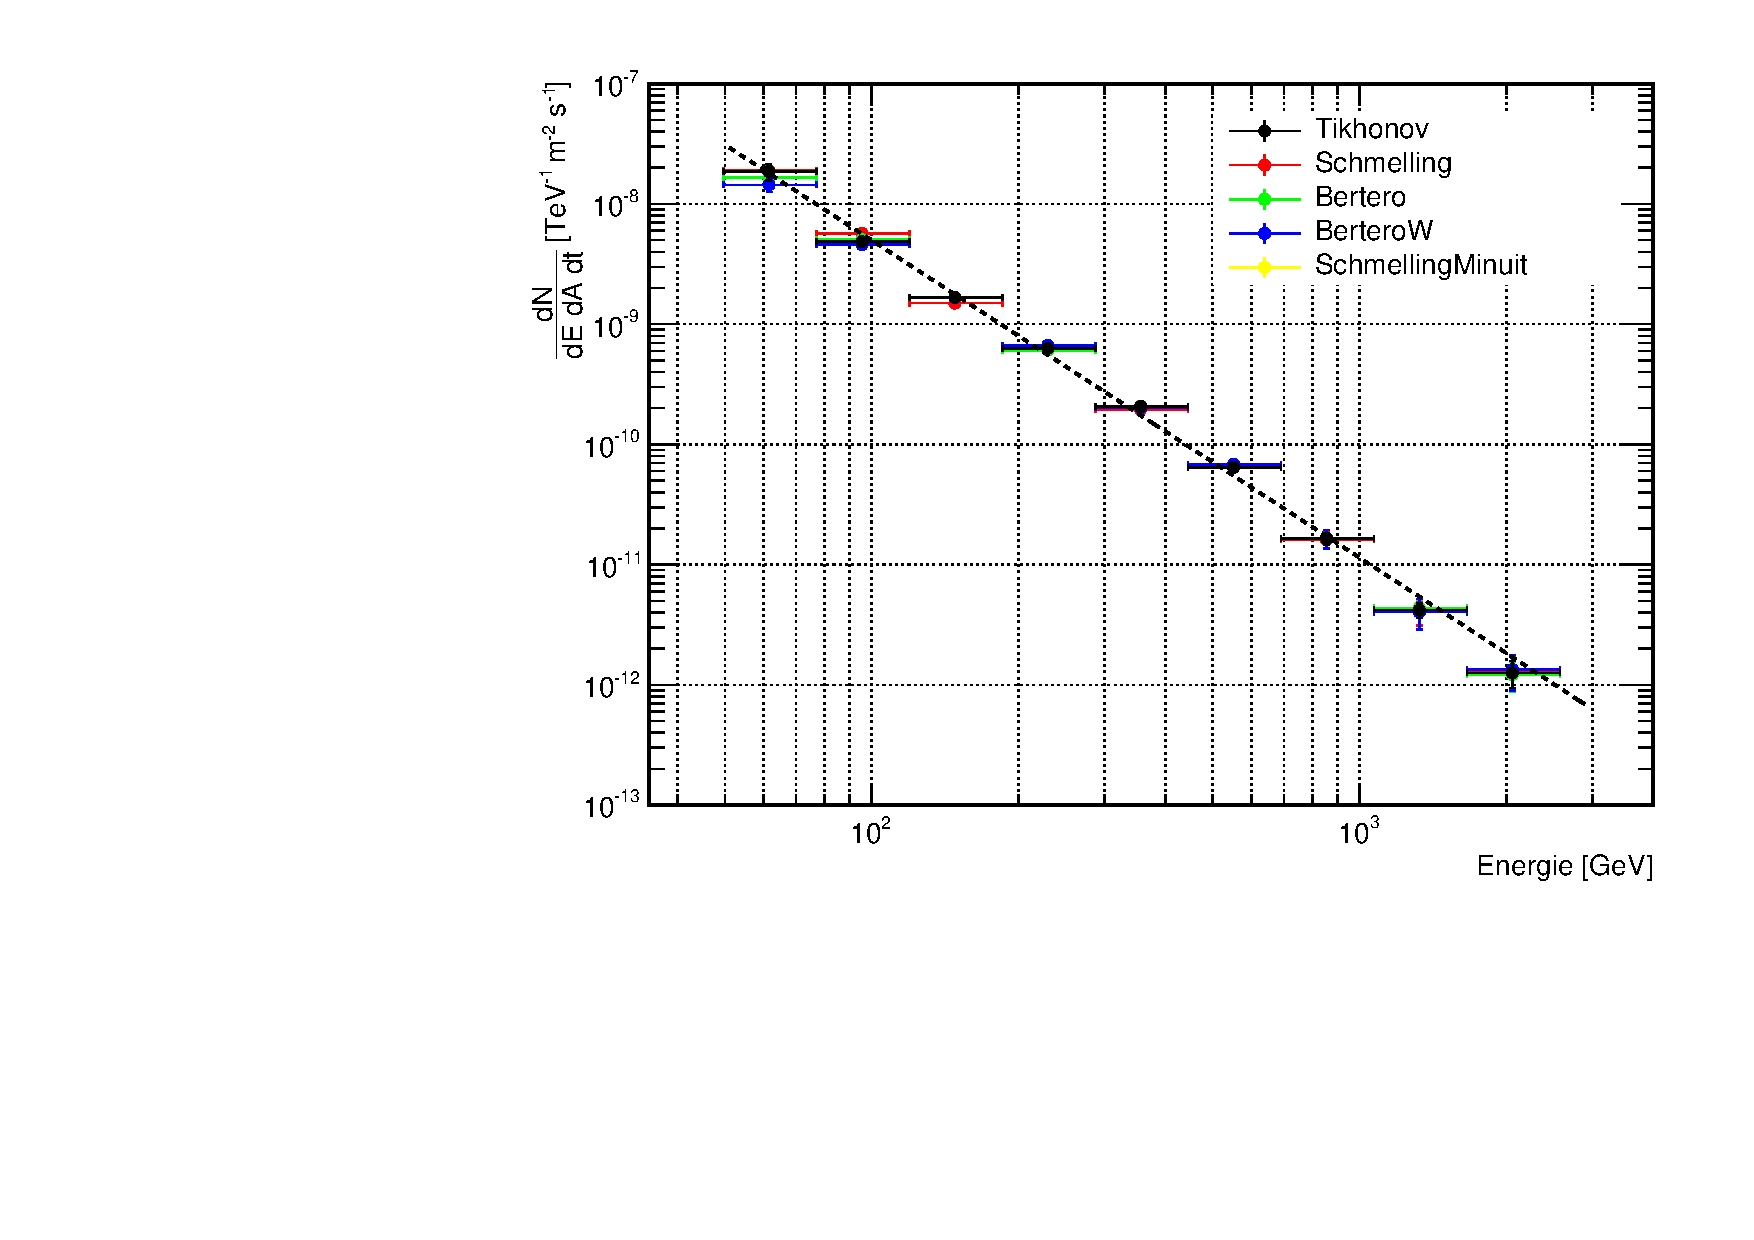
\includegraphics[width=0.8\textwidth]{./Plots/04_MrkAnalyse/Datenset2/Spektrum_Mrk421.pdf}
    \caption{Entfaltetes Mrk 421-Spektrum im Zeitraum vom 18.3.2012 bis zum 25.4.2012 mit allen möglichen Regularisierungsmethoden.}
    \label{Datenset2_CombunFold_Mrk421}
\end{figure}

Es wurde der Fit, der in der Entfaltung mit Tikhonov-Regularisierung erstellt wurde, zusätzlich dargestellt, da diese Regularisierungsmethode in den meisten Fällen die besten Ergebnisse lieferte.
Folgende Funktion wurde angenommen:

\begin{equation}
 \frac{dN}{dE\,dA\,dt}=f_0\left( \frac{E}{r} \right)^\alpha.
\end{equation}

Der Fit lieferte das Ergebnis:

\begin{equation}
 \frac{dN}{dE\,dA\,dt}=(2,74 \pm 0,06) \cdot 10^{-10}\left( \frac{E}{\SI{0,3}{TeV}} \right)^{-2.64 \pm 0,03} \si{TeV^{-1}\,s^{-1}\,cm^{-2}}.
\end{equation}


\FloatBarrier

\subsection{Datenset 1}
\label{subsec:Datenset_1}
Der folgende Teil beschreibt die Analyse der Daten vom 25.2.2012 und 29.2.2012.
Da diese Daten eine andere PSF haben als die Daten aus dem Datenset 2, gibt es eigene MCs dafür und die Daten müssen getrennt von Datenset 2 analysiert werden.
Die Daten an diesen zwei Tagen haben ebenfalls einen Zenitbereich unter 35°.

\subsubsection{Datencheck}
Der Datencheck für diese Daten geschieht analog zum Datencheck des Datensets 2. 
Tabelle \ref{tab:Datenset1-Mrk421} zeigt an welchen Tagen Mrk 421-Daten den Datencheck überstanden haben und für die Analyse zur Verfügung stehen. 

\begin{table}[!h]
\centering
\caption{Übersicht über alle nach dem Datencheck zur Verfügung stehenden Daten von Mrk~421 aus Datenset 1.}
\label{tab:Datenset1-Mrk421}
\begin{tabular}{ll}
  \toprule
  Monat & Tage\\
  \midrule
  \midrule
Februar & 25., 29.\\
  \bottomrule
\end{tabular}
\end{table}


Tabelle \ref{tab:Datenset1} zeigt wieviel Mrk 421-/Crab- und Background-Daten den Datencheck überstanden haben.


\begin{table}[!h]
\centering
\caption{Übersicht über alle nach dem Datencheck zur Verfügung stehenden Daten von Mrk~421, Crab und Background aus Datenset 1.}
\label{tab:Datenset1}
\begin{tabular}{lc}
  \toprule
  Quelle & Obersvationszeit [min]\\
  \midrule
  \midrule
  Mrk 421 & 70\\
  \midrule
  Crab & 20\\
  \midrule
  0FGLJ0631 & 3 \\
  1ES1011 & 172 \\
  HB89 & 87 \\
  PG1553 & 115 \\
  PKS1222 & 106 \\
  SegueJ & 401 \\
  \bottomrule
  \bottomrule
\end{tabular}
\end{table}

\subsubsection{Lichtkurve}
Mit Hilfe von Crab-Daten wurden wieder die Einstellungen für die Lichtkurve von Mrk 421 bestimmt.
Es wurde nur an einem Tag zwischen dem 25.2.2012 und dem 29.2.2012 Crab beobachtet.
Deswegen beinhaltet die Lichtkurve von Crab nur $\SI{20}{min}$ an Crab-Daten (vgl. \autoref{Datenset1_LC_Crab}).

\begin{figure}
    \centering
    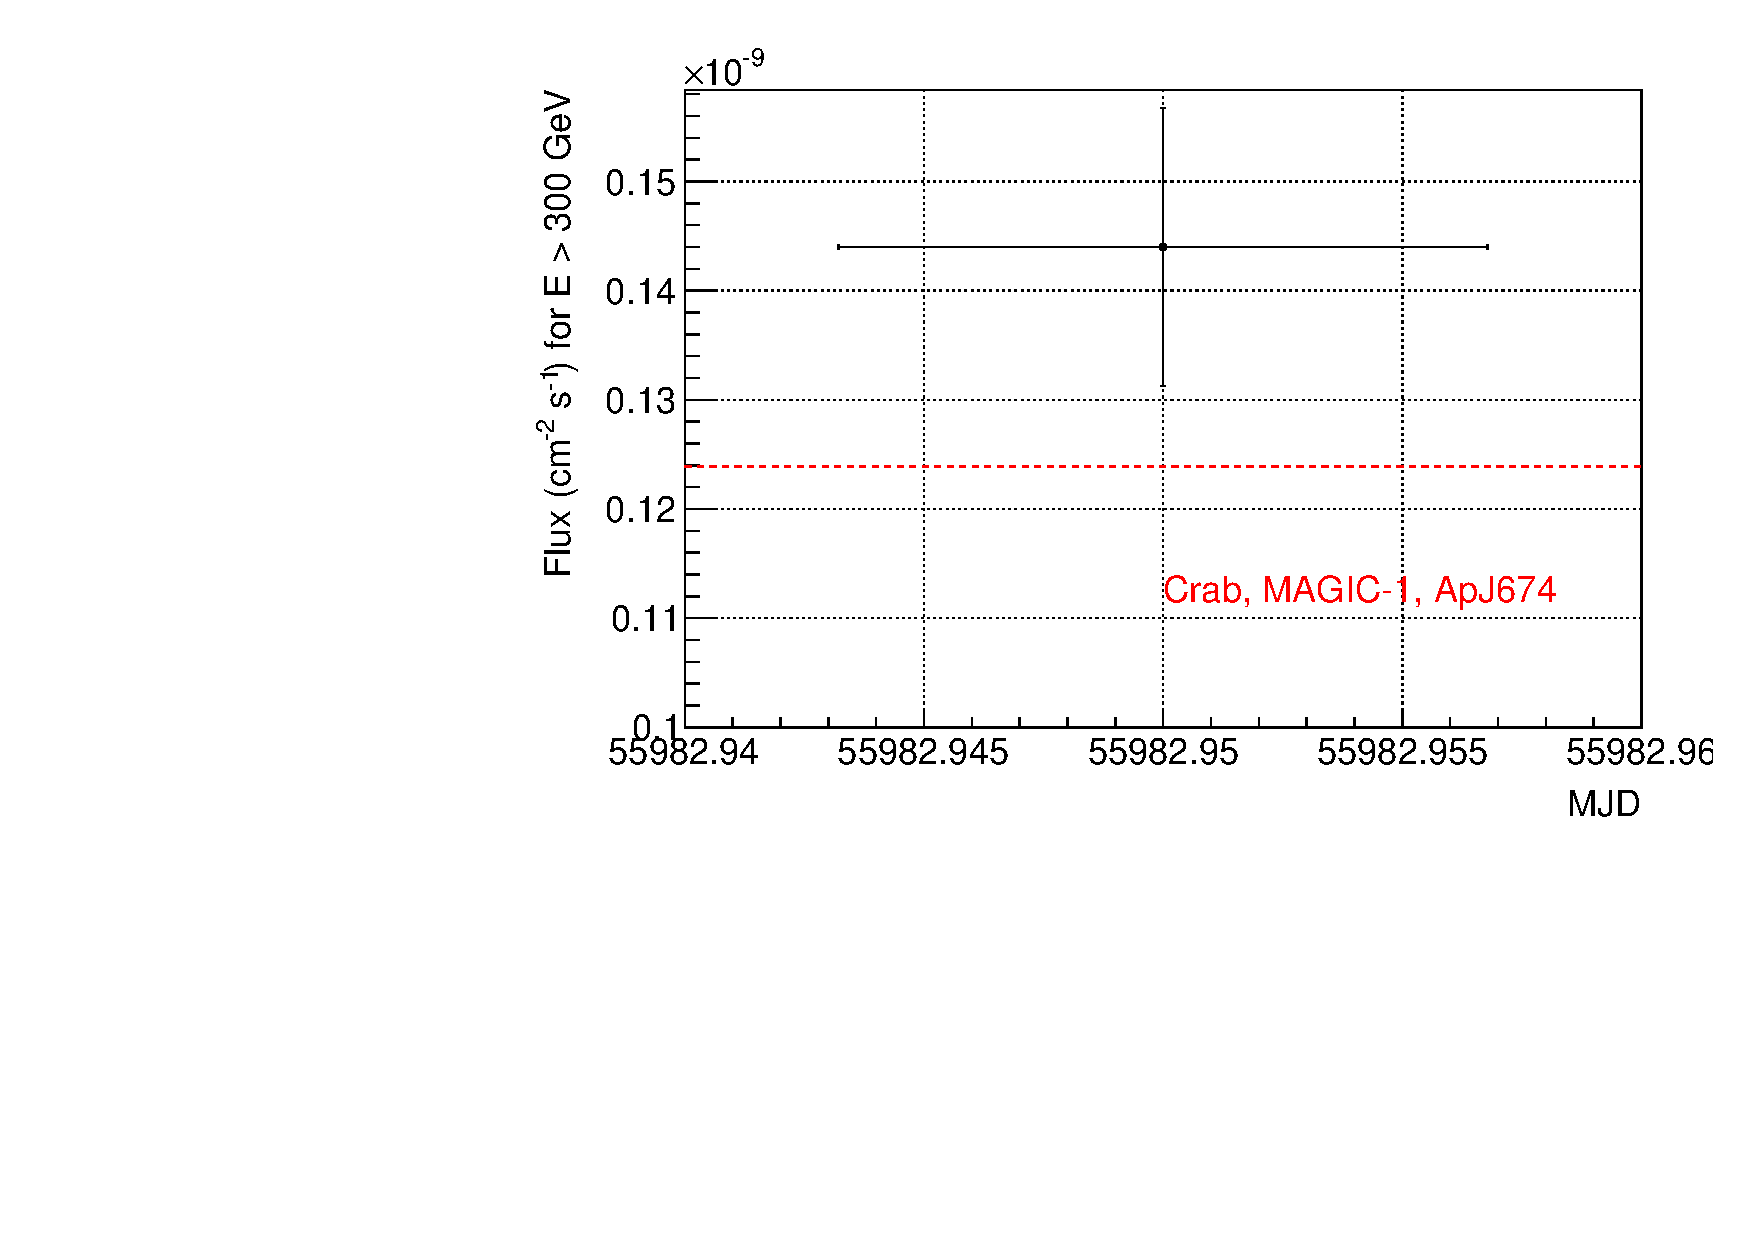
\includegraphics[width=0.8\textwidth]{./Plots/04_MrkAnalyse/Datenset1/Datenset1_LC_Crab.pdf}
    \caption{LC von Crab im Zeitraum vom 25.2.2012 bis zum 29.2.2012.}
    \label{Datenset1_LC_Crab}
\end{figure}

Die Lichtkurve von Mrk 421 befindet sich in Abb.\ref{Datenset1_LC_Mrk421}.

\begin{figure}
    \centering
    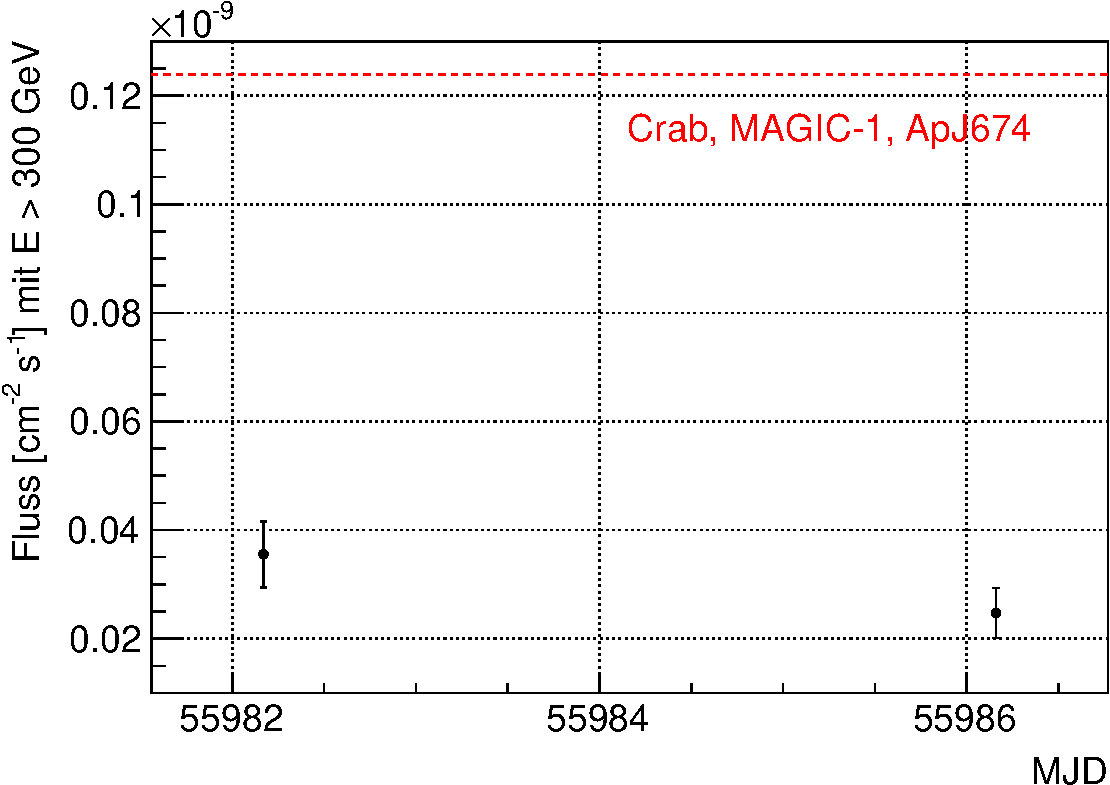
\includegraphics[width=0.8\textwidth]{./Plots/04_MrkAnalyse/Datenset1/Datenset1_LC_Mrk421.pdf}
    \caption{Lichtkurve von Mrk 421 im Zeitraum vom 25.2.2012 bis zum 29.2.2012.}
    \label{Datenset1_LC_Mrk421}
\end{figure}

Es ist zu sehen, dass der Fluss an diesen beiden Tagen verglichen mit den ersten Tagen aus Datenset 2 sehr niedrig ist.



\FloatBarrier

\subsubsection{Spektrum}
Analog zu Datenset 2 wurde auch wieder ein Spektrum bestimmt.
Das Resultat befindet sich in Abb.\ref{Datenset1_Spektrum_Mrk421}

\begin{figure}
    \centering
    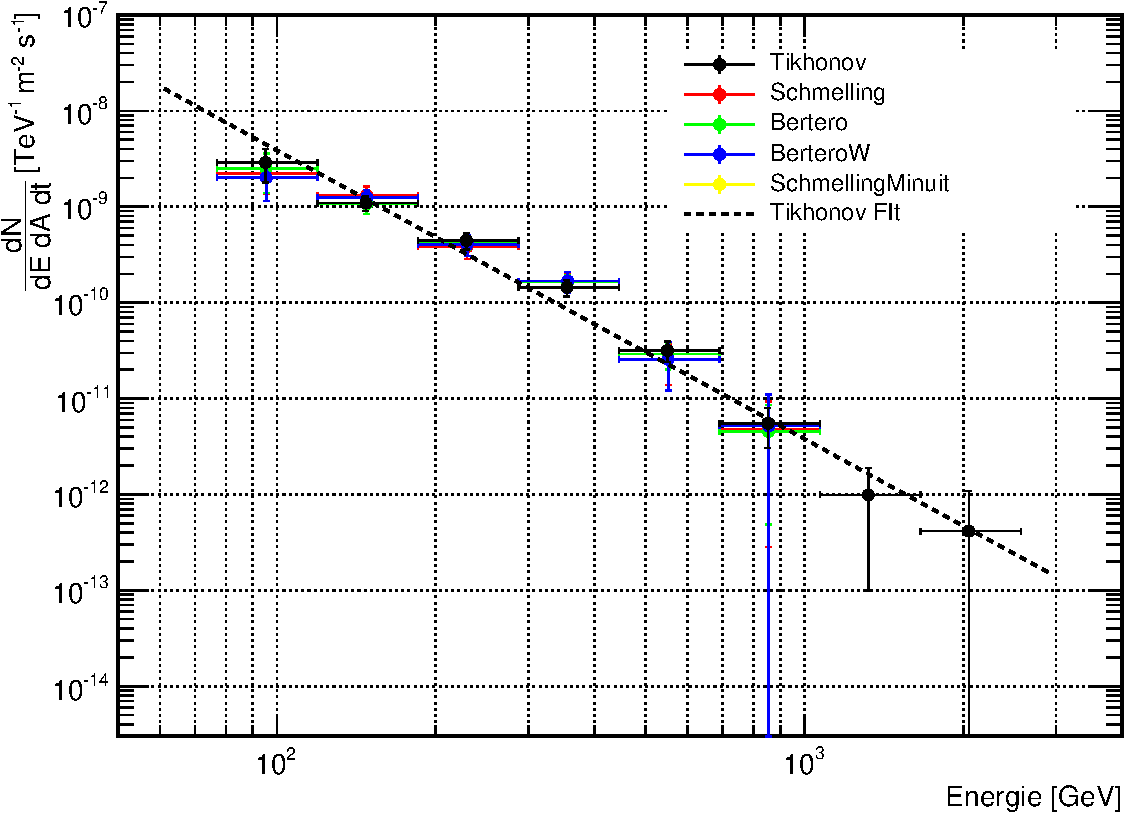
\includegraphics[width=0.8\textwidth]{./Plots/04_MrkAnalyse/Datenset1/Spektrum_Mrk421.pdf}
    \caption{Entfaltetes Spektrum von Mrk 421 im Zeitraum vom 25.2.2012 bis zum 29.2.2012.}
    \label{Datenset1_Spektrum_Mrk421}
\end{figure}

Es ist zu sehen, dass die Entfaltungen ohne Tikhonov-Regularisierung im hohen Energiebereich nicht mehr funktionieren.
Auch bei kleinen Energien unterscheiden sie sich etwas.
Aufgrund des großen Energiebereichs, in dem die Entfaltung mit Tikhonov-Regularisierung Ergebnisse liefert, wird wieder dieser Fit der Punkte eingezeichnet.
Der Fit lieferte folgendes Ergebnis:

\begin{equation}
 \frac{dF}{dE}=(1,42 \pm 0,11) \cdot 10^{-11}\left( \frac{E}{0,3 \si{TeV}} \right)^{-3.01\pm 0,14} \si{TeV^{-1}\,s^{-1}\,cm^{-2}}.
\end{equation}

Aufgrund der kurzen Observationszeit wurde keine Entfaltung der Crab-Daten vorgenommen.

\FloatBarrier

\subsection{Datenset 4}
\label{subsec:Datenset_4}
Dieses Datenset beinhaltet die ersten Daten, die von Mrk 421 nach dem Austausch der MAGIC-I-Kamera genommen wurden. 
Genauso wie Datenset 1 umfasst dieses Datenset nur wenige Tage. 
An drei Tagen wurde Mrk 421 im Stereo-Modus observiert. 

\subsubsection{Datencheck}
Der Datencheck für diese Daten geschieht analog zum Datencheck des Datensets 2. 
Tabelle \ref{tab:Datenset4} zeigt, welche Mrk 421-/Crab- und Background-Daten nach dem Datencheck übrig sind und Tabelle \ref{tab:Datenset4-Mrk421} an welchen Tage die Mrk 421-Daten genommen wurden.

\begin{table}[!h]
\centering
\caption{Übersicht über alle an nach dem Datencheck zur Verfügung stehenden Daten von Mrk~421 aus Datenset 4.}
\label{tab:Datenset4-Mrk421}
\begin{tabular}{ll}
  \toprule
  Monat & Tage\\
  \midrule
  \midrule
Dezember & 15., 19., 23.\\
  \bottomrule
\end{tabular}
\end{table}


\begin{table}[!h]
\centering
\caption{Übersicht über alle an nach dem Datencheck zur Verfügung stehenden Daten von Mrk~421, Crab und Background aus Datenset 4.}
\label{tab:Datenset4}
\begin{tabular}{lc}
  \toprule
  Quelle & Observationszeit [min]\\
  \midrule
  \midrule
  Mrk 421 & 74\\
  \midrule
  Crab & 852\\
  \midrule
  1ES0229 & 221 \\
  NGC1275 & 112 \\
  SegueA & 900  \\
  \bottomrule
  \bottomrule
\end{tabular}
\end{table}

\subsubsection{Lichtkurve}
Die Lichtkurve von Crab befindet sich in \autoref{Datenset4_LC_Crab}. 
Es ist zu sehen, dass diese Lichtkurve mit dem mittleren Fluss von Crab gut übereinstimmt.
Die Lichtkurve von Mrk 421 in \autoref{Datenset4_LC_Mrk421} 
Wie zu sehen ist, liegen auch hier die Flüsse niedrig.

\begin{figure}
    \centering
    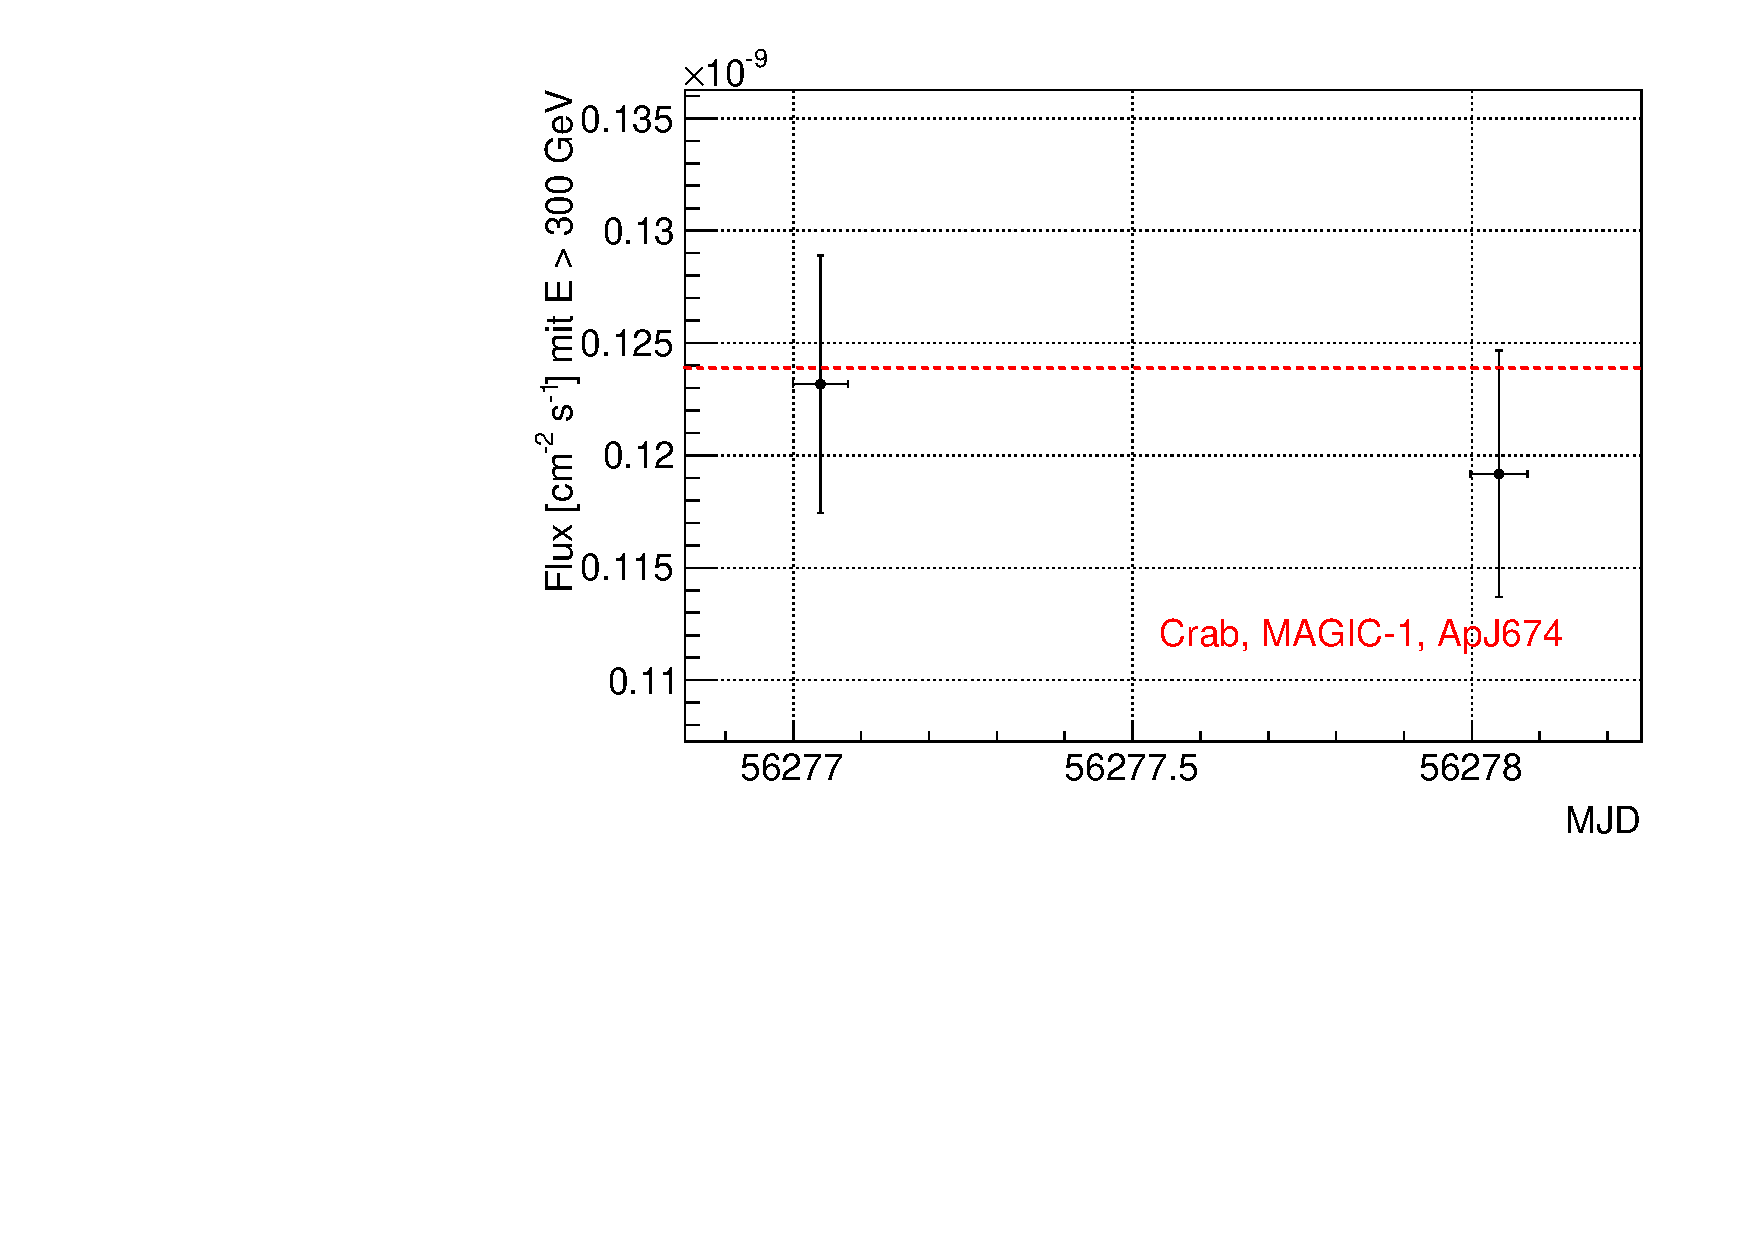
\includegraphics[width=0.8\textwidth]{./Plots/04_MrkAnalyse/Datenset4/Datenset4_LC_Crab.pdf}
    \caption{Lichtkurve Crab im Zeitraum vom 15.12.2012 bis zum 23.12.2012.}
    \label{Datenset4_LC_Crab}
\end{figure}

\begin{figure}
    \centering
    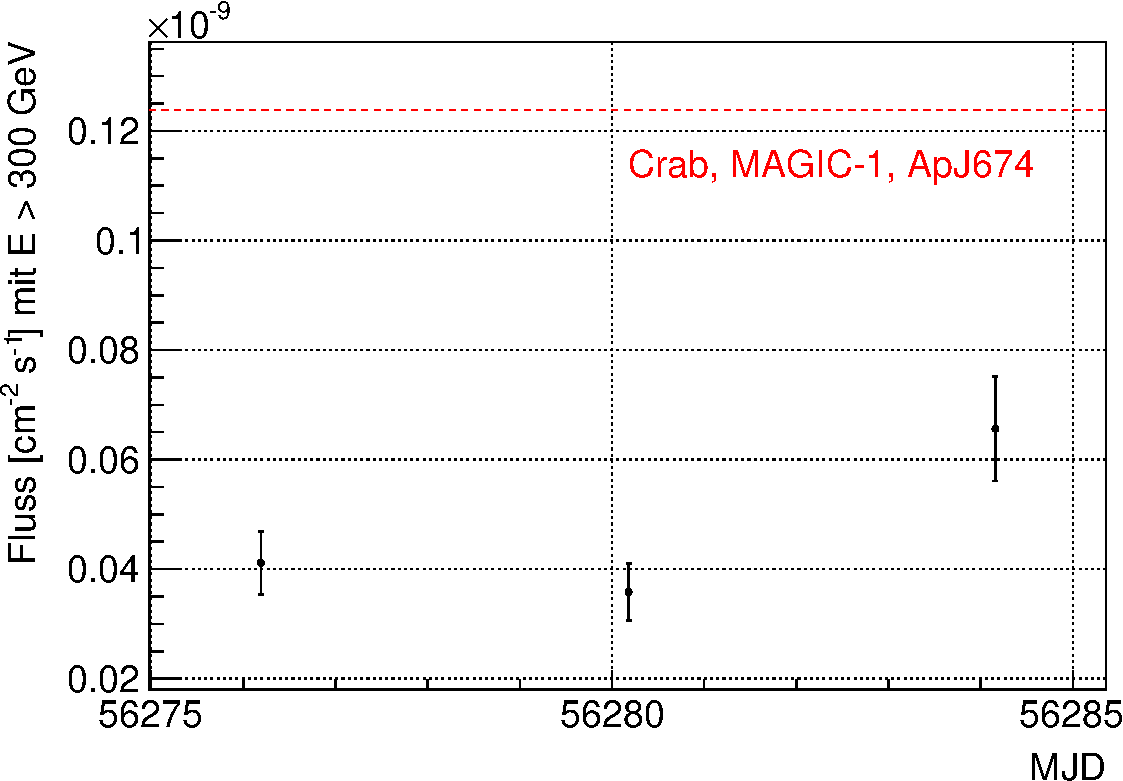
\includegraphics[width=0.8\textwidth]{./Plots/04_MrkAnalyse/Datenset4/Datenset4_LC_Mrk421.pdf}
    \caption{Lichtkurve Mrk 421 im Zeitraum vom 15.12.2012 bis zum 23.12.2012.}
    \label{Datenset4_LC_Mrk421}
\end{figure}


\subsubsection{Spektrum}
Das entfaltete Spektrum von Mrk 421 befindet sich in Abb.\ref{Datenset4_Spektrum_Mrk421}.

\begin{figure}
    \centering
    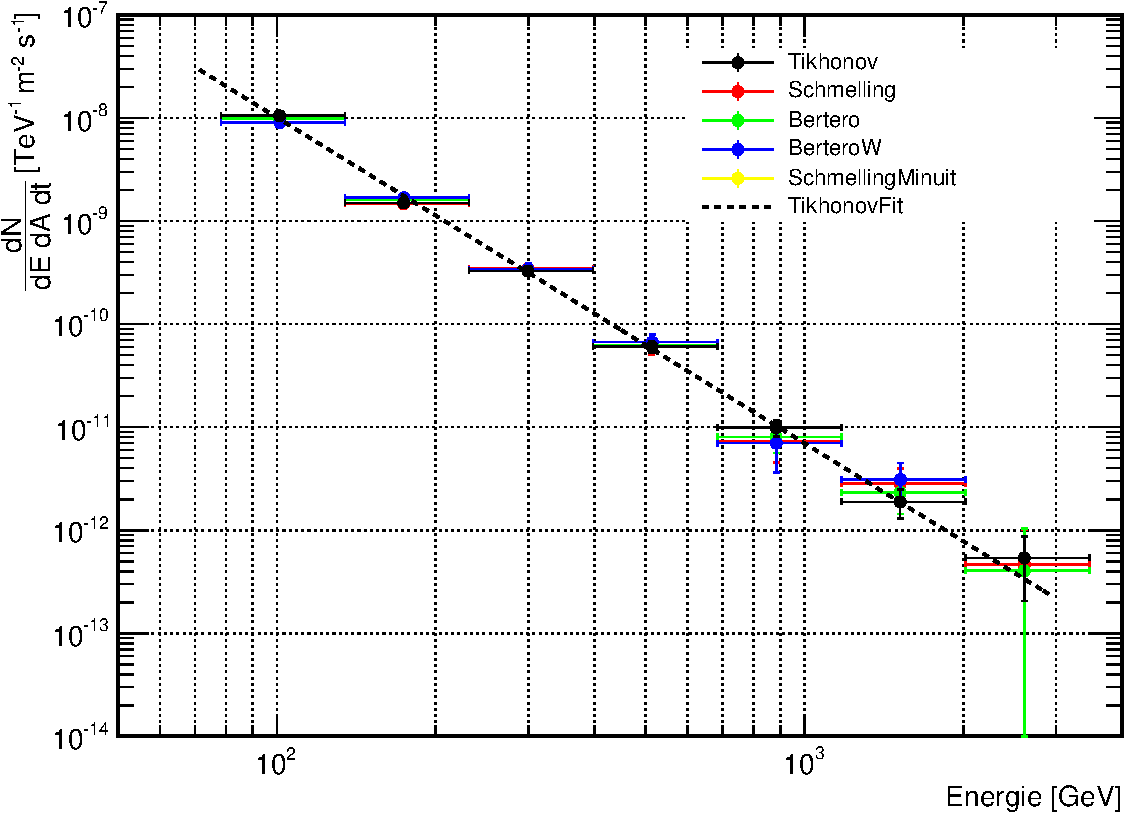
\includegraphics[width=0.8\textwidth]{./Plots/04_MrkAnalyse/Datenset4/Datenset4_Spektrum_Mrk421.pdf}
    \caption{Entfaltetes Spektrum von Mrk 421 im Zeitraum vom 15.12.2012 bis zum 23.12.2012.}
    \label{Datenset4_Spektrum_Mrk421}
\end{figure}

Der Fit des entfalteten Spektrums mit Tikhonov-Regularisierung liefert folgendes Ergebnis:

\begin{equation}
 \frac{dF}{dE}=(3,14 \pm 0,15) \cdot 10^{-10}\left( \frac{E}{0,3 \si{TeV}} \right)^{-3.16\pm 0,07} \si{TeV^{-1}\,s^{-1}\,cm^{-2}}.
\end{equation}


\FloatBarrier

\subsection{Datenset 3}
\label{subsec:Datenset_3}

\subsubsection{Datencheck}
Der Datencheck für die Mono-Daten geschieht analog zum Datencheck der anderen Datensets.
Die Analyse beruht auf Daten auf Star-Level und nicht Superstar-Level wie vorher.
Tabelle \ref{tab:Datenset3-Mrk421} und Tabelle \ref{tab:Datenset3} zeigen, welche Mrk 421-und Background-Daten nach dem Datencheck übrig sind.
Ein Beobachtung von Crab gab es zu diesem Zeitraum nicht.

\begin{table}[!h]
\centering
\caption{Übersicht über alle nach dem Datencheck zur Verfügung stehenden Daten von Mrk~421 aus Datenset 3.}
\label{tab:Datenset3-Mrk421}
\begin{tabular}{ll}
  \toprule
  Monat & Tage\\
  \midrule
  \midrule
Mai & 23., 25., 26., 27.\\
Juni & 15,. 19. \\
  \bottomrule
\end{tabular}
\end{table}


\begin{table}[!h]
\centering
\caption{Übersicht über alle nach dem Datencheck zur Verfügung stehenden Daten von Mrk~421, Crab und Background aus Datenset 3}
\label{tab:Datenset3}
\begin{tabular}{lc}
  \toprule
  Quelle & Observationszeit [min]\\
  \midrule
  \midrule
  Mrk 421 & 333\\
  \midrule
  1ES1959 & 360 \\
  AE-Aqr & 54  \\
  HD215227 & 649 \\
  M87 & 64 \\
  \bottomrule
  \bottomrule
\end{tabular}
\end{table}

\subsubsection{Energieschätzung}
Im Vergleich zu der Stereo-Analyse müssen für die Mono-Analyse ältere Programme benutzt werden.
Die RFs für die \texttt{Disp}-Bestimmung und Gamma-Hadron-Separation werden mit Hilfe von \textit{Osteria} erstellt.
Im Gegensatz zur Standardanalyse werden keine Look-Up-Tables zur Energieschätzung benutzt, sondern ebenfalls ein RF.

\subsubsection{Lichtkurve}
Nachdem den Ereignissen eine Hadroness, ein \texttt{Disp}-Wert sowie eine geschätzte Energie zugeordnet worden sind, wird nach Anwendung eines Hadroness-Schnittes wieder eine Lichtkurve erstellt.
Dies geschieht mit Hilfe des Programms \textit{Fluxlc}.
Obwohl keine Crab-Daten zur Verfügung standen, um die Einstellungen für die Lichtkurve mit einem bekannten Fluss zu überprüfen, wird eine Lichtkurve für Mrk 421 erstellt.
Abb.\ref{Datenset3_LC_Mrk421} zeigt die Lichtkurve für Mrk 421.

\begin{figure}
    \centering
    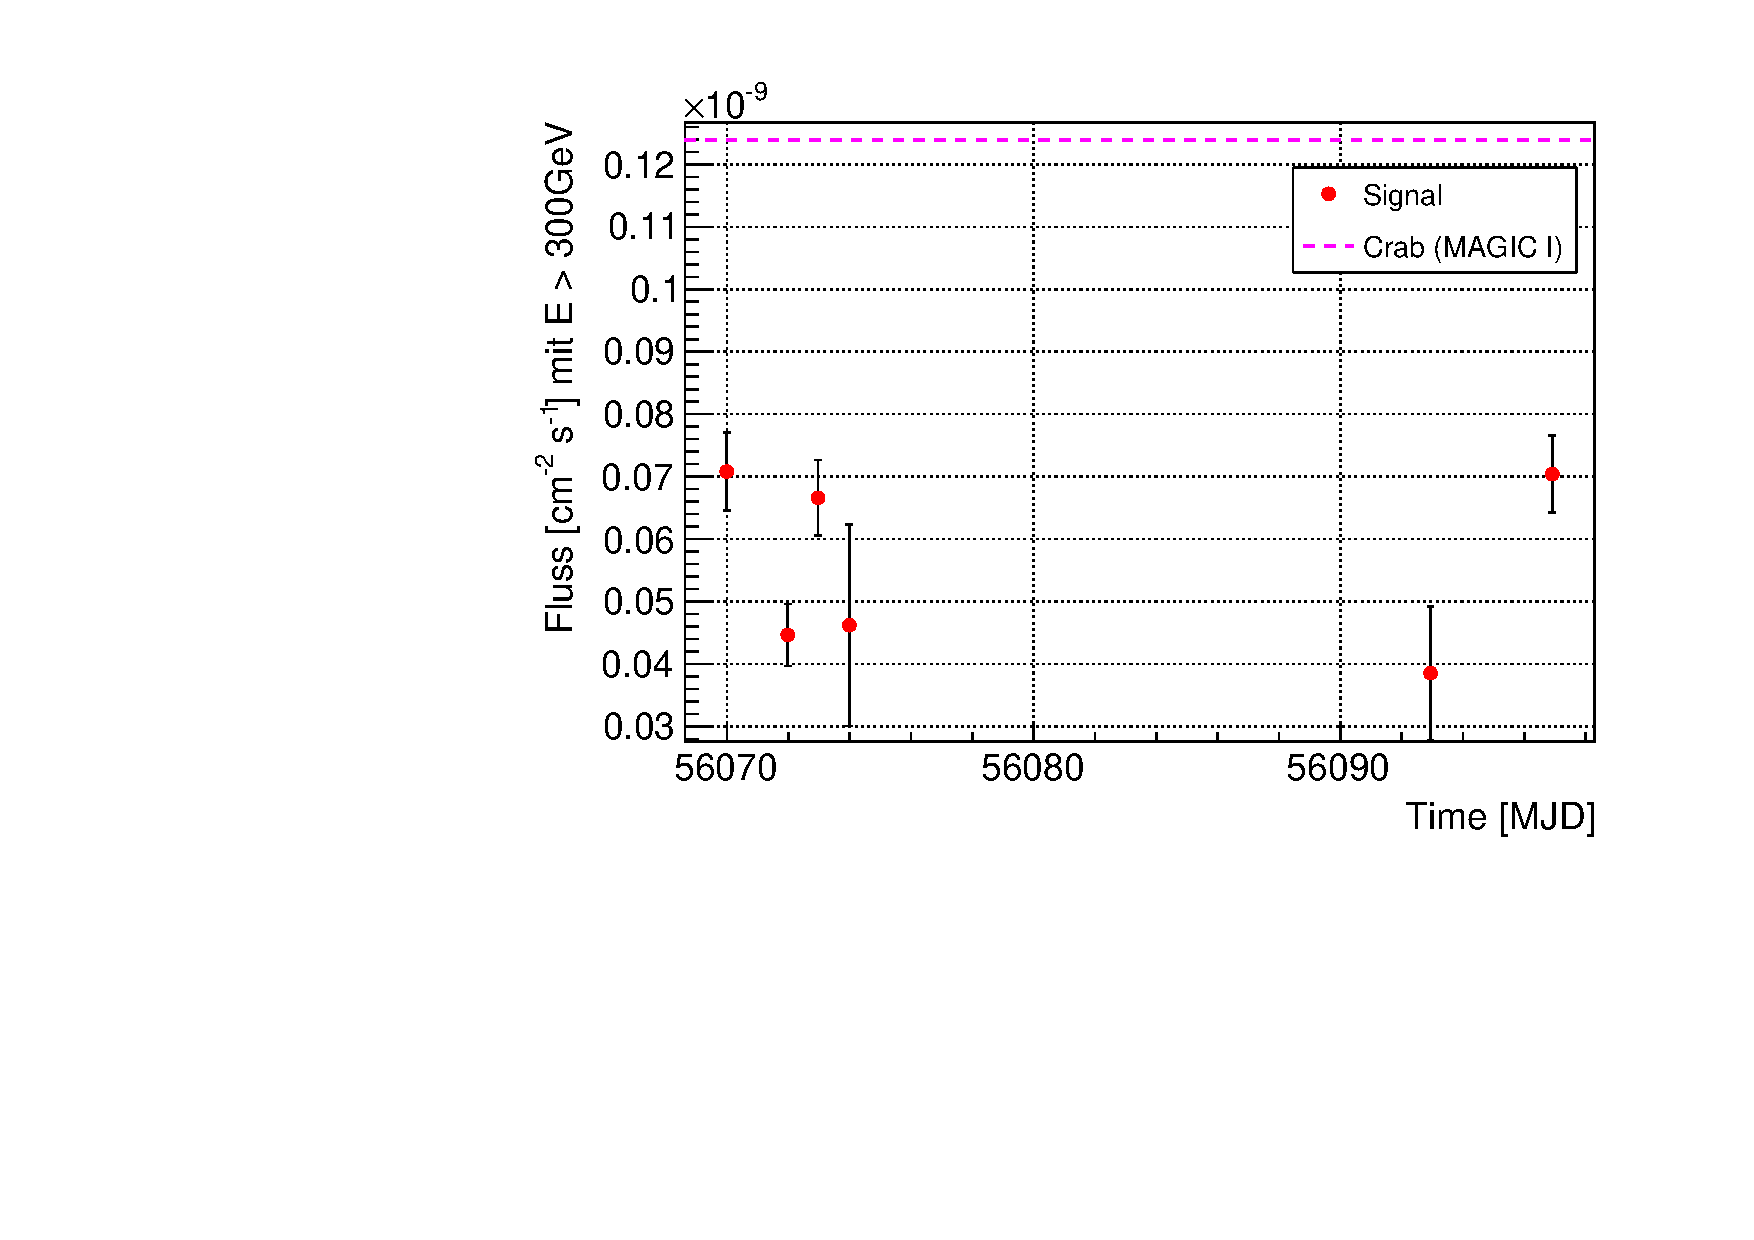
\includegraphics[width=0.8\textwidth]{./Plots/04_MrkAnalyse/Datenset3/Datenset3_Mrk421_LC.pdf}
    \caption{Lichtkurve von Mrk 421 im Zeitraum vom 23.05.2012 bis zum 19.05.2012.}
    \label{Datenset3_LC_Mrk421}
\end{figure}

Es zeigt sich, dass der Fluss von Mrk 421 in diesem Zeitbereich genau wie in den anderen Zeitbereichen ebenfalls sehr niedrig ist.


\subsubsection{Spektrum}

Wie in Abb.\ref{Datenset3_Spektrum_Mrk421} zu sehen ist, werden die Daten abschließend wieder entfaltet.

\begin{figure}
    \centering
    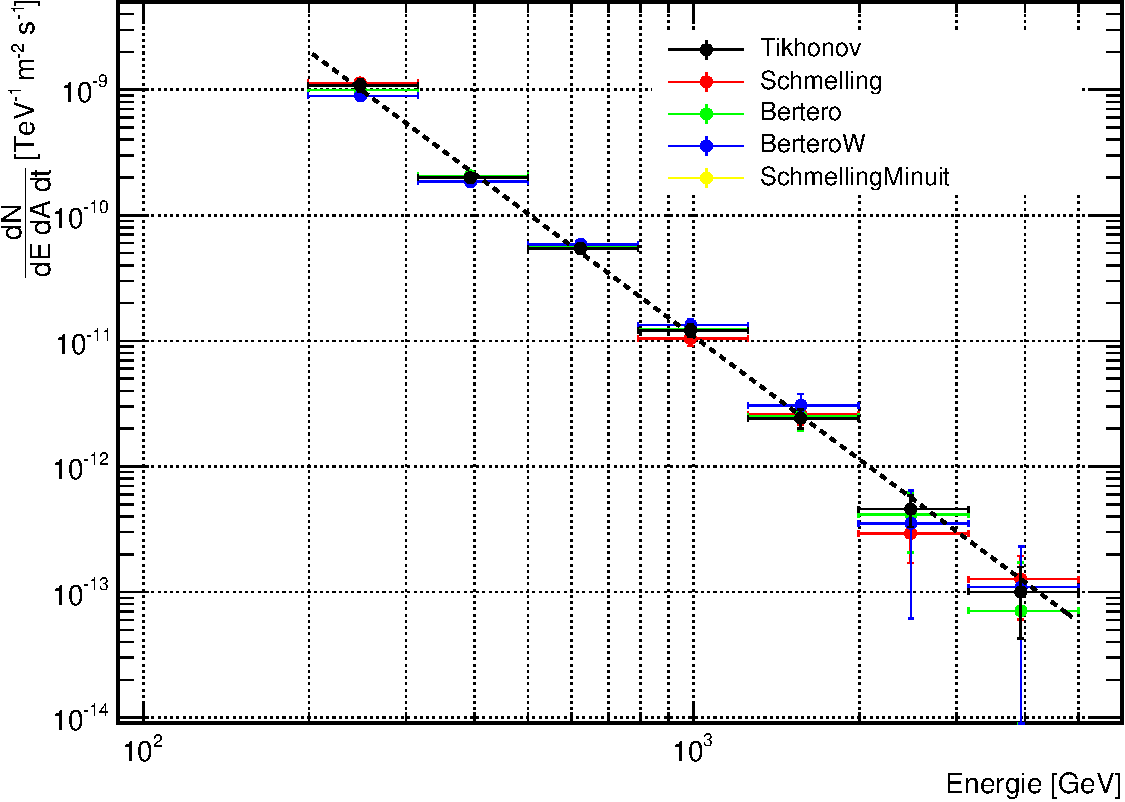
\includegraphics[width=0.8\textwidth]{./Plots/04_MrkAnalyse/Datenset3/Datenset3_Mrk421_Spektrum.pdf}
    \caption{Spektrum Mrk 421.}
    \label{Datenset3_Spektrum_Mrk421}
\end{figure}

Der Fit an die Datenpunkte nach einer Entfaltung mit Tikhonov-Regularisierung liefert folgendes Ergebnis:

\begin{equation}
 \frac{dF}{dE}=(5,42 \pm 0.23) \cdot 10^{-10}\left( \frac{E}{\SI{0,3}{TeV}} \right)^{(-3.25 \pm 0.09)} \si{TeV^{-1}\,s^{-1}\,cm^{-2}}.
\end{equation}

\FloatBarrier


\section{Zusammenfassung der Ergebnisse und Vergleich der Datensets}
\label{LC_Alles}

Nachdem für jedes Datenset einzelne Lichtkurven erstellt worden sind, sieht man in Abb.\ref{Alles_LC_Mrk421} nun alle Daten in einer Lichtkurve dargestellt.
Da zwischen dem 20.06.2012 und dem 10.12.2012 keine Daten von Mrk 421 genommen wurden, weil die MAGIC-I-Kamera außer Betrieb war und das Upgrade durchgeführt wurde, befindet sich eine große Lücke in der Lichtkurve.

\begin{figure}
    \centering
    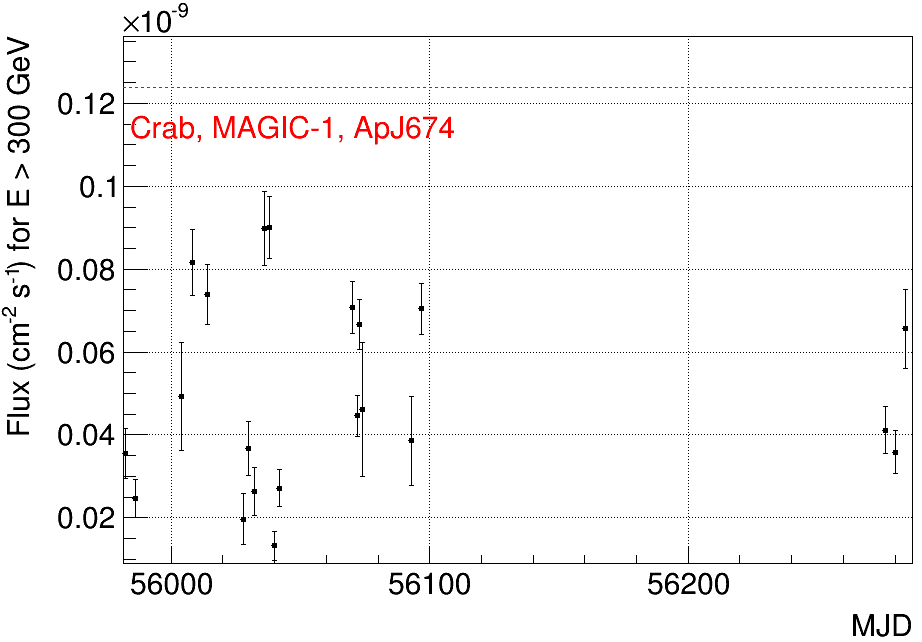
\includegraphics[width=0.8\textwidth]{./Plots/04_MrkAnalyse/Alles_LC.png}
    \caption{LC Mrk 421.}
    \label{Alles_LC_Mrk421}
\end{figure}

Es ist zu sehen, dass alle Datenpunkte etwa auf dem gleichen niedrigen Niveau liegen.
Der Fluss von Crab wird zu keinem Zeitpunkt erreicht.
Physikalisch interessante Phänomene wie Flares wurden im gesamten Jahr 2012 von MAGIC nicht beobachtet.
%Im April 2013 trat beispielsweise ein Flare auf.
Verglichen mit dem gesamten Fluss von MAGIC zwischen Dezember 2004 und Dezember 2009 in \cite{DissBackes} ist der Fluss 2012 auf einem niedrigen Niveau.
Im Dezember 2006 war er an vielen Tagen genauso niedrig.

Im Gegensatz zu den Flares 2007 und 2008, bei denen der Fluss bis zu 20 mal so hoch war wie zu ruhigen Zeiten \cite{DissBackes}, ist der Fluss 2012 konstant niedrig.

Ein Vergleich mit dem Fluss zwischen Januar und Mai 2009 \cite{DissDiego} liefert ebenfalls das Ergebnis, dass sich sich Mrk 421 in einem ruhigen Zustand befindet.

In Tabelle \ref{tab:SpektraleIndizes} befinden sich die spektralen Indizes der Entfaltung der einzelnen Datensets.
Die spektralen Indizes der Datensets 1,3 und 4 beschreiben ein steiles Spektrum mit relativ niedrigem hochenergetischem Fluss.
Datenset 2 hat einen kleineren spektralen Index, d.h. das Spektrum ist härter, wobei der Fluss wie oben erwähnt, den Crab-Fluss nicht erreicht.


\begin{table}[!h]
\centering
\caption{Vergleich der spektralen Indizes und Flusskonstanten der einzelnen Datensets.}
\label{tab:SpektraleIndizes}
\begin{tabular}{lll}
  \toprule
  Datenset & Normierung $\left[\si{TeV^{-1}\,cm^{-2}\,s^{-1}}\right]$ & spektraler Index\\
  \midrule
  \midrule
Datenset 1 & $(1,42\pm 0,11)\cdot 10^{-10}$ & -3,01 $\pm$ 0,14 \\
Datenset 2 & $(2,74\pm 0,06)\cdot 10^{-10}$ & -2,64 $\pm$ 0,03 \\
Datenset 3 & $(5,42\pm 0,23)\cdot 10^{-10}$ & -3,25 $\pm$ 0,09 \\
Datenset 4 & $(3,14\pm 0,15)\cdot 10^{-10}$ & -3,16 $\pm$ 0,07 \\
  \bottomrule
\end{tabular}
\end{table}


\chapter{Multiwellenlängen-Untersuchungen}
\label{chapter:MWL}
In diesem Kapitel werden neben der MAGIC Lichtkurve noch Lichtkurven anderer Experimente in anderen Wellenlängen dargestellt, die im Rahmen einer Multiwellenlängen -Kampagne (MWL-Kampagne)  genommen wurden und mit den MAGIC Daten verglichen.
Es stehen dazu Daten im Energiebereich zwischen Radiowellen und Very High Energy Gamma Rays zur Verfügung.
Die MWL-Kampagne fand zwischen dem 23.12.2011 und dem 01.06.2012 statt und war die Fortsetzung einer früheren MWL-Kampagne von 2009.
Genauso wie während der Vorgängerkampagne befindet sich innerhalb der Beobachtungszeit kein Flare.
Das Ziel dieser Kampagne ist, den Fluss und die spektrale Entwicklung der Breitband-Emission über eine lange Zeitspanne zu untersuchen, wobei jeweils tageweise Daten genommen wurden.
Während es viele Untersuchungen zu den Emissionsszenarien bei Flares gibt (siehe z.B. \cite{Mrk421Flare}), wurde der ruhige Zustand von Mrk 421 nicht sehr ausführlich untersucht (abgesehen von \cite{MWL2009}).
Mit Hilfe von diesen Daten, können grundlegende Emissionsprozesse untersucht werden.

Blazare wie Mrk 421 sind in allen Wellenlängen sehr variabel.
Die Spektrale Energieverteilung (SED) wird von der Jet-Emission dominiert und besitzt eine zweihöckrige Struktur.
Der erste Höcker findet sich bei niedrigen Energien [Radio, optisch, Röntgenstrahlen] und der andere bei höheren Energien [Röntgen, Gamma, VHE].
Während der Ursprung des niederenergetischen Höckers Synchrotron-Emission von relativistischen Elektronen ist, ist der Ursprung des hochenergetischen Höckers noch nicht genau bekannt.
Sowohl leptonische als auch hadronische Modelle versuchen die Struktur zu erklären.
Um Modelle für den hochenergetischen Höcker zu bestimmen, sind weiterhin Beobachtungen in verschiedenen Wellenlängen nötig. 
 

\section{Teilnehmende Experimente an der MWL-Kampagne}
Von den folgenden Experimenten, die sich an dieser Kampagne beteiligt haben, stehen für diese Analyse Daten zur Verfügung:

\begin{itemize}
 \item MAGIC: eigene Analyse
 \item \textit{Swift}/XRT: \textit{Swift} ist ein Satellitenexperiment mit dem Ziel GRBs zu detektieren und zu untersuchen.
  Dabei liegt die Priorität darauf, den Ursprung von GRBs zu finden, die Entwicklung der GRBs und die Wechselwirkung mit der Umgebung zu untersuchen und die GRBs zu klassifizieren.
  Dazu sind drei Instrumente an Bord, die in verschiedenen Wellenlängen sensitiv sind. 
  Mit \textit{Swift} können Gammastrahlung, Röntgenstrahlung, UV-Strahlung und optisches Licht detektiert werden.
  Mit Hilfe des Burst Alert Telescope (BAT) werden Teilchen mit Energien zwischen $\SI{15}{keV}$ und $\SI{150}{keV}$ untersucht.
  Das UV/Optical Telescope (UVOT) detektiert im sichtbaren und im UV-Bereich (170-$\SI{600}{nm}$).
  Die für diese Analyse vorliegenden Daten sind vom Xray Telescope (XRT), womit Röntgenstrahlung mit einer Energie zwischen $\SI{0,3}{keV}$ und $\SI{10}{keV}$ detektiert wird.\cite{Swift}
 \item OVRO: Das Owens Valley Radio Observatory (OVRO) befindet sich in der Nähe von Bishop in Kalifornien im Osten der Sierra Nevada.
  Es ist ein Radioteleskop mit einem Durchmesser von $\SI{40}{m}$, welches bei $\SI{15}{GHz}$ operiert.
  Ziel dieses Experimentes ist das Monitoring von ca. 1200 Blazaren.
  Dabei wird jede Quelle in einem Abstand von zwei Tagen regelmäßig beobachtet.
  Diese Daten werden dann mit den Daten, die mit \textit{Fermi} von den gleichen Quellen aufgenommen wurden, verglichen und Korrelationen in der Variabilität gesucht.
  Letztendlich ist ein genaueres Verständnis von Emissionsprozessen in AGNs das Ziel.\cite{OVRO}
 \item Metsahovi: Metsahovi ist ein Radioteleskop mit einem Spiegeldurchmesser von $\SI{14}{m}$. 
  Es befindet sich in Finnland, in Kirkkonummi, und beobachtet Frequenzen zwischen $\SI{2}{GHz}$ und $\SI{150}{GHz}$.
  Mit dem Teleskop werden hauptsächlich extragalaktische Quellen beobachtet, aber auch die Sonne und es nimmt an VLBI (Very Large Baseline Interferometry)-Beobachtungen teil.\cite{Metsahovi}
 \item Optische Teleskope: Für diese Analyse stehen die Daten einiger optischer Teleskope zur Verfügung, deren Datennahme unter Einsatz des R-Filters geschah.
  Im Folgenden werden diese Teleskope aufgelistet:
 \begin{itemize}
  \item Crimean: Das Crimean Astrophysical Observatory befindet sich in Nauchny auf der Krim, Ukraine, und beherbergt verschiedene optische Teleskope.\cite{Crimean}
  \item KVA: Das Kungliga Vetenskaplika Academy (KVA)-Teleskop befindet sich genauso wie die MAGIC Teleskope auf dem Roque de los Muchachos auf La Palma.
    Es handelt sich um ein Teleskop mit einem Spiegeldurchmesser von $\SI{35}{cm}$.
    Die Daten sind alle im Johnson R-Band genommen.\cite{KVA}
  \item Perkins: Das Perkins Telescope ist ein $\SI{72}{inch}$ ($\SI{1,83}{m}$)-Teleskop, das zum Lowell Observatory in Arizona, USA, gehört.
    Mit diesem Teleskop werden vor allem Wide-Field-Bilder aufgenommen und es dient der Multi-Objekt-Spektroskopie.
    Unter anderem soll mit diesem Teleskop auch die variable Natur von Blazaren untersucht werden.\cite{Perkins}
  \item ROVOR: Das Remote Observatory for Variable Object Research (ROVOR) gehört zur Brigham Young University.
    Es handelt sich um ein optisches Teleskop mit einem Spiegeldurchmesser von $\SI{16}{inch}$ ($\SI{0,41}{m}$) und es befindet sich $\SI{12}{km}$ nordwestlich von Delta (Utah).
    Es wurde gebaut um variable Objekte wie AGNs dauerhaft zu monitoren und damit die existierenden Modelle für AGNs zu verbessern.
    ROVOR nimmt am Gamma Ray Burst Coordinate Network (GCN) teil und beobachtet die Afterglows im optischen Wellenlängenbereich.\cite{ROVOR}
  \item St. Petersburg: Das Pulkovo Astronomical Observatory befindet sich südlich von St. Petersburg auf einer Höhe von $\SI{75}{m}$ über NN.\cite{StPetersburg}
  \item TeB: Das Bradford Robotic Telescope ist Teil des Observatorio del Teide auf Teneriffa, Kanarische Inseln. 
    Es befindet sich auf einer Höhe von $\SI{2400}{m}$ und wird robotisch betrieben.\cite{TeB}
  \item NMSkies: New Mexico Skies bietet einen Standort und Support für dort aufgestellte Remote Teleskope. 
    Das Teleskop NMSkies GRAS-001 befindet sich in Mayhill, New Mexico, USA.\cite{NMSkies}
 \end{itemize}

 \item \textit{Fermi}: Das Large Area Telescope (LAT) befindet sich an Bord des \textit{Fermi} Gamma-Ray Space Telescope und detektiert sowohl Gamma-Strahlen als auch geladene kosmische Strahlen.
  Das Teleskop beinhaltet einen Antikoinzidenzdetektor, durch den das Photon im Gegensatz zur geladenen kosmischen Strahlung wechselwirkungsfrei fliegt. 
  Danach wechselwirkt es mit Atomen in einer der Schichten aus Wolfram-Folie und produziert ein Elektron-Positron-Paar, welches getrackt wird.
  Die finale Energie dieses Elektron-Positron-Paars wird dann in einem Kalorimeter gemessen.
  Das Entdecken und Überwachen von variablen Quellen und GRBs sowie die Erstellung von aktuellen Katalogen von hochenergetischen Quellen gehören zu den Hauptzielen von \textit{Fermi}.\cite{Fermi} 
\end{itemize}

\section{Vergleich der Lichtkurven}
In \autoref{LC_MWL} befinden sich die Lichtkurven der verschiedenen Experimente, die im Zeitraum zwischen dem 23.12.11 (MJD: 55918) und dem 01.06.12 (MJD: 56079) gemessen wurden.

\begin{sidewaysfigure}
%\begin{sidewaysfigure}
%\begin{figure}
    \centering
    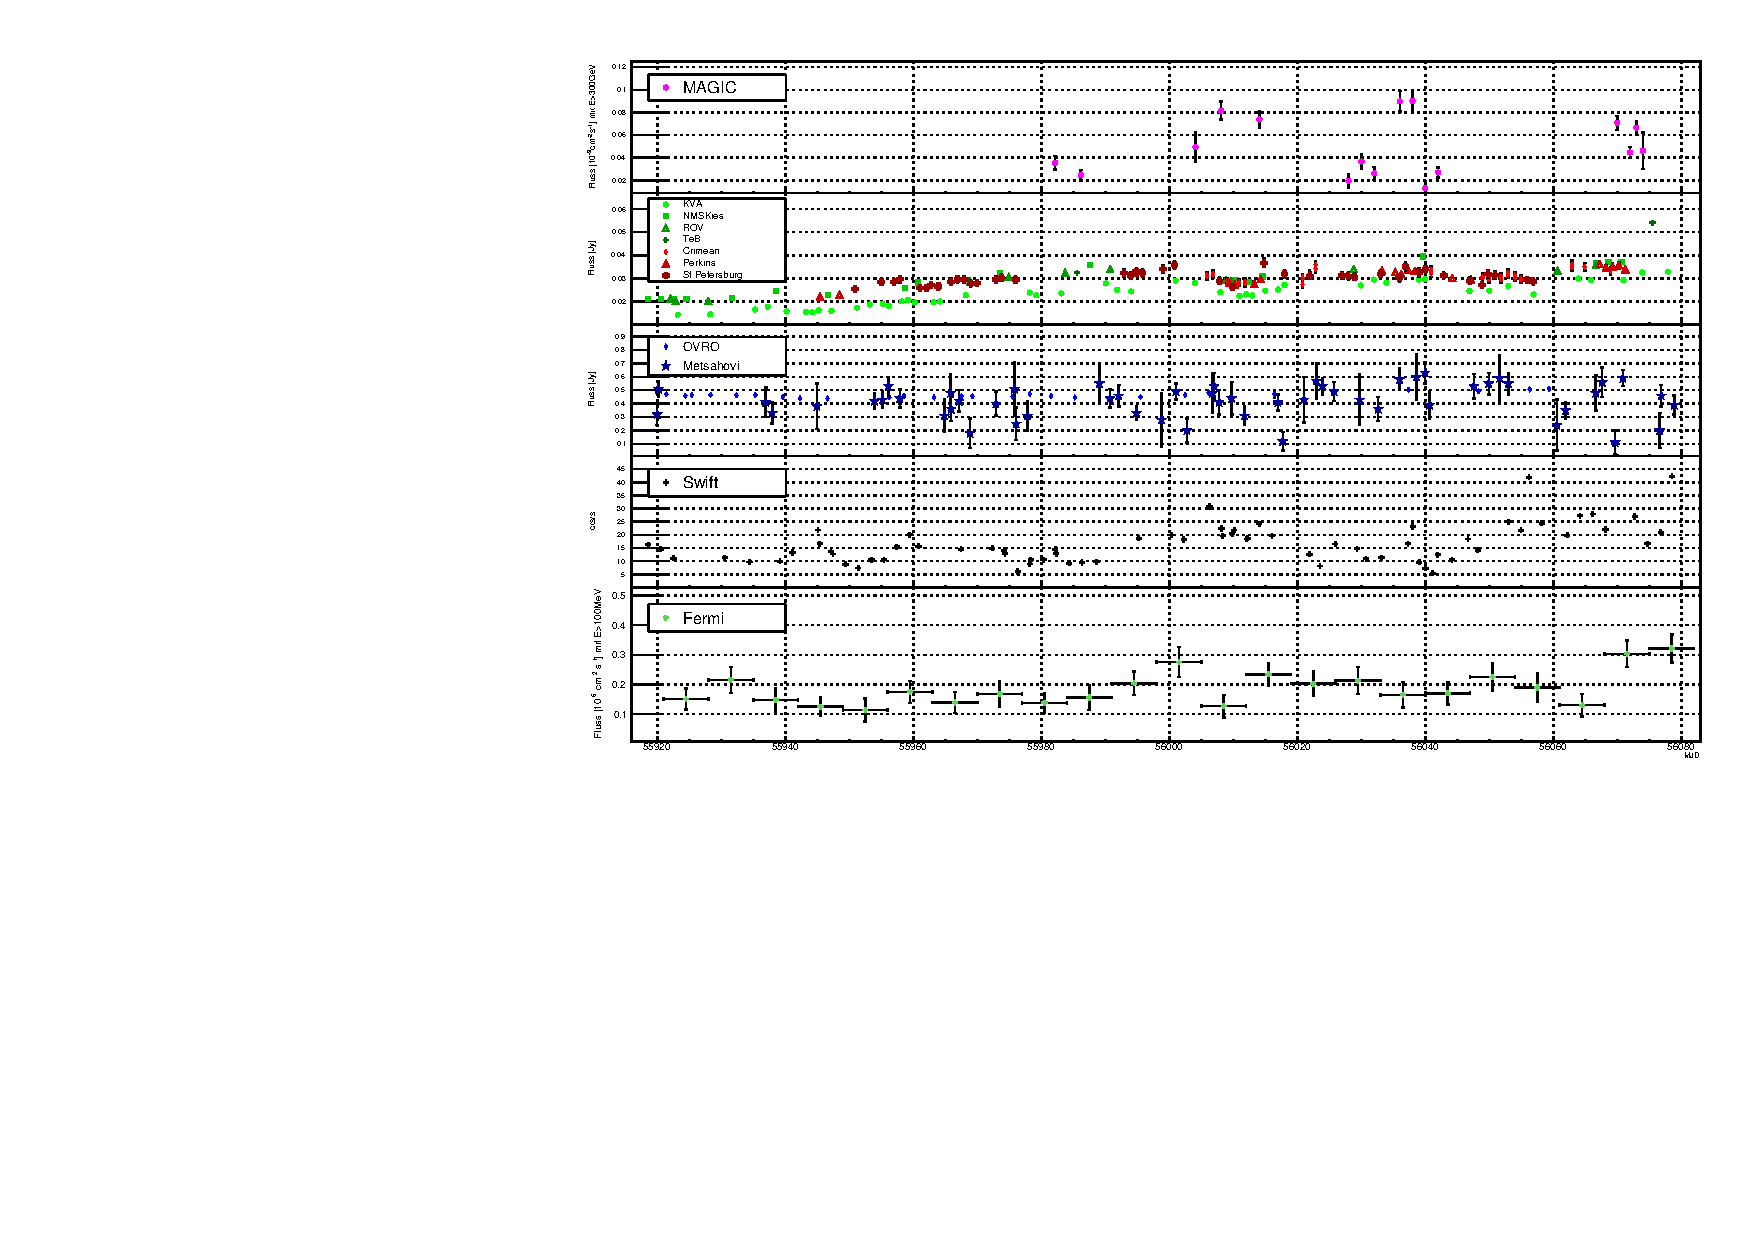
\includegraphics[width=1\linewidth]{./Plots/05_MWL/LC_final.pdf}
    \caption{Alle Lichtkurven, die während der MWL-Kampagne aufgenommen wurden: von oben nach unten: VHE, Optische Teleskope, Radio, Röntgen, Gamma}
    \label{LC_MWL}
%\end{figure}
\end{sidewaysfigure}

Leider hat MAGIC an nur 16 Tagen davon Daten genommen, weswegen die Lichtkurve im Vergleich zu den anderen Experimenten recht kurz ist, bzw. große Lücken aufweist.
Auf den ersten Blick weist die Lichtkurve eine variable Struktur auf, was in \autoref{sec:Variabilitätsuntersuchung} noch getestet wird.

Die optischen Lichtkurven der verschiedenen Teleskope liegen insgesamt auf einem ähnlichen Niveau, wobei KVA immer etwas niedriger ist.
Die meisten Daten stammen von KVA (Beobachtung an 48 Tagen), dem St. Petersburger Teleskop (Beobachtung an 46 Tagen) und dem Crimean Astrophysical Observatory (Beobachtung an 35 Tagen).
Die Variabilität im Fluss zwischen den verschiedenen Teleskopen ist ähnlich. 
Einige Schwankungen sind zu erkennen und zum Ende der Lichtkurve nimmt das Niveau etwas zu.

Im Radiobereich sind bei den OVRO-Daten kaum Variabilitäten zu erkennen. 
Die Daten von Metsahovi unterliegen größeren Schwankungen, sind aber auch mit einem größeren Fehler behaftet.
Quantativ wird dieses Verhalten in \autoref{sec:Variabilitätsuntersuchung} gezeigt.

Die Daten des Röntgenteleskops \textit{Swift}, welches eine sehr konstante Datennahme aufweist, zeigen einen eher variablen Fluss, was im Folgenden noch überprüft wird.

Die Daten von \textit{Fermi}-LAT sind gemittelte Resultate von einer Woche, zeigen also keine täglichen Schwankungen.
Aufgrund des Mittelns und der dadurch Nicht-Vergleichbarkeit mit den anderen Experimenten wird im Folgenden keine Variabilität berechnet.

Insgesamt kann man erkennen, dass die Variabilität in der VHE-Lichtkurve auf Zeitskalen von ca. einem Tage auftritt, während der Fluss im optischen oder Röntgenbereich eher innerhalb einer Woche ansteigt und wieder abnimmt. 
Die Radiolichtkurven weisen keine sichtbaren Variabilitäten auf.

\section{Variabilitätsuntersuchung}
\label{sec:Variabilitätsuntersuchung}
Obwohl es in der Zeit der MWL-Kampagne zu keinem Flare kam, sind die Daten von Mrk421 variabel.
Um quantifizieren zu können, wie variabel die Daten sind, wird für jeden Energiebereich die Fractional Variability nach \cite{Vaughan} ausgerechnet.
Der Wert für die Fractional Variability $F_{var}$ wird mit $S$: der Standardabweichung der N Flussmessungen, $\langle \sigma_{err} \rangle$: dem mittleren quadrierten Fehler und $\langle x \rangle^2$: dem Quadrat des mittleren Photonflusses berechnet:

\begin{equation}
 F_{var}=\sqrt{\frac{S^2-\langle \sigma_{err} \rangle^2}{\langle x \rangle^2}}.
\end{equation}

Der Fehler davon ist \cite{FehlerVariability} entnommen: 

\begin{equation}
 \Delta F_{var}=\sqrt{F_{var}^2+err(\sigma_{NXS}^2)}-F_{var}
\end{equation}

mit $err(\sigma_{NXS}^2)$ aus \cite{Vaughan}:

\begin{equation}
 err(\sigma_{NXS}^2)=\sqrt{\left(\sqrt{\frac{2}{N} \frac{\langle \sigma_{err}^2 \rangle}{\langle x \rangle^2}} \right)^2 + \left( \sqrt{\frac{\langle\sigma_{err}^2 \rangle}{N} \frac{2F_{var}}{\langle x \rangle}} \right)^2}.
\end{equation}

Damit die Berechnung von $F_{var}$ stabil ist, wird eine Mindestanzahl von 20 gemessenen Datenpunkten empfohlen.
Obwohl die MAGIC-Daten nur aus 16 gemessenen Punkten bestehen, wird trotzdem zum Vergleich einmal die Variabilität ausgerechnet.
Die berechneten Werte für die Variabilität $F_{var}$ mit Fehler $\Delta F_{var}$ sowie die Anzahl der Messpunkte $N$ befindet sich in \autoref{tab:Variabilitäten}, bzw. in \autoref{LC_Variabilities}.


\begin{table}[!h]
\centering
\caption{Anzahl der Messpunkte, sowie die berechneten Variabilitäten für die verschiedenen Lichtkurven.}
\label{tab:Variabilitäten}
\begin{tabular}{llccc}
  \toprule
  Wellenlänge & Experiment & N & $F_{var}$ & $\Delta F_{var}$\\
  \midrule
  \midrule
  Radio & Metsahovi & 55 & 0,1390 & 0,0319 \\
  &OVRO & 27 & 0,0381 & 0,0036 \\
  optisch &KVA & 48 & 0,2227 & 0,0031 \\
  &St. Petersburg & 46 & 0,0768 & 0,0067 \\
  &Crimean & 35 & 0,0586 & 0,0075 \\
  Röntgen & \textit{Swift} & 70 & 0,4428 & 0,0015\\
  Gamma & MAGIC & 16 & 0,4913 & 0,0380 \\
  \bottomrule
\end{tabular}
\end{table}


\begin{figure}
    \centering
    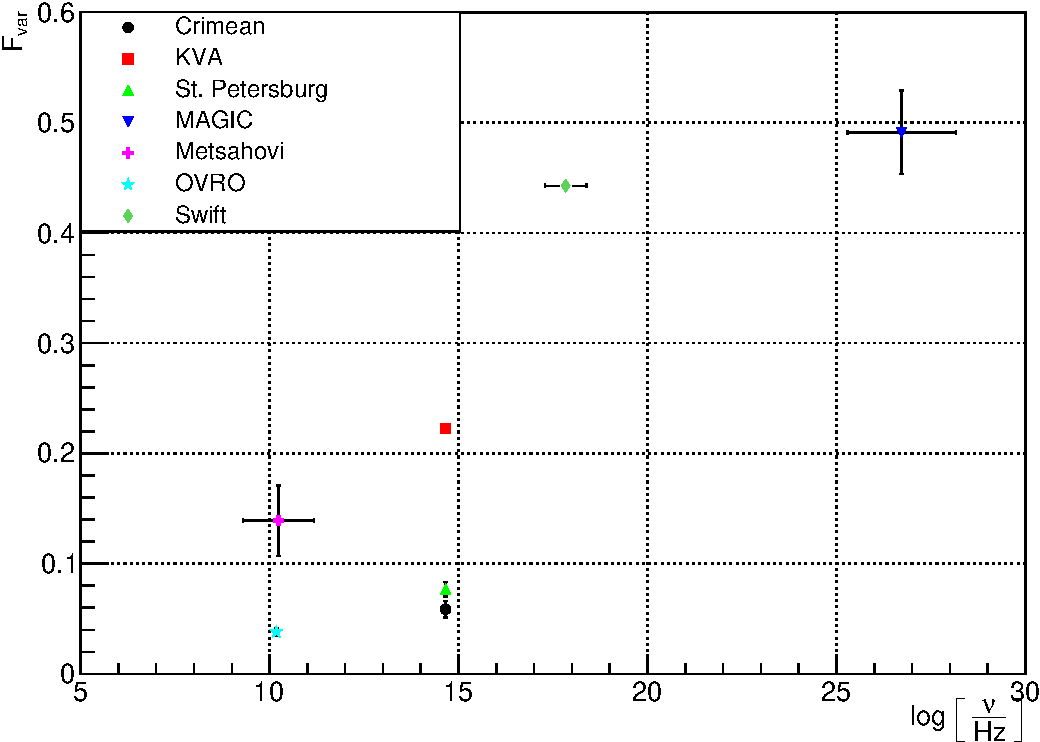
\includegraphics[width=0.9\textwidth]{./Plots/05_MWL/PlotVariabilities.pdf}
    \caption{Darstellung der Variabilitäten in den verschiedenen Wellenlängen.
    Es ist zu erkennen, dass mit steigender Frequenz die Variabilität zunimmt.
    Die Variabilität der Röntgen- und der Gammastrahlung ist auf einem ähnlichen Niveau.}
    \label{LC_Variabilities}
\end{figure}

\autoref{LC_Variabilities} zeigt die Variabilitäten in den einzelnen Wellenlängen, wobei die Breite des x-Balkens den Energiebereich angibt, in dem die jeweiligen Instrumente messen.
\autoref{LC_Variabilities} zeigt, dass die Variabilität von Mrk421 im Radio- und im optischen Bereich sehr niedrig ist, während die AGN im Röntgen- und im Gamma-Bereich Variabilität aufweist, wobei beachtet werden muss, dass der Wert für MAGIC mit Vorsicht betrachtet werden muss, da die Anzahl der Datenpunkte niedrig ist.
Insgesamt lässt sich sagen, dass die Variabilitäten mit steigender Frequenz ebenfalls ansteigen.
Die hier berechneten Variabilitäten sind ähnlich zu den berechneten Werten für Mrk421 von 2009 \cite{MWL2009}.

\chapter{Zusammenfassung}
\label{chapter:Ergebnisse}
Im Rahmen dieser Arbeit wurde zunächst eine Einführung in die Astroteilchenphysik gegeben. 
Die kosmische Strahlung wurde beschrieben und Quelle dieser Strahlung vorgestellt.
Anschließend wurden mögliche Beschleunigungsmechanismen dargestellt.
Die Überleitung zum Gebiet der Gammaastronomie führt in das eigentliche Forschungsthema dieser Arbeit ein.
Dieses Thema umfasst die Analyse des Aktiven Galaktischen Kerns (AGN) Markarian~421, welcher nachfolgend vorgestellt wird.

Ein essenzieller Grundstein für diese Analyse sind die speziell angepassten Monte Carlo-Simulationsdaten.
Diese wurden im Zeitraum der Doktorarbeit in Dortmund für die gesamte MAGIC-Kollaboration produziert und an aktuelle Hardwareveränderungen des Teleskops angepasst.
Beginnend mit der Luftschauersimulation mit \textit{CORSIKA} werden nacheinander die Reflektor-Simulation und die Kamera- und Elektronik-Simulation vorgestellt.
Diese Programme benötigen spezielle Eingabeparameter, welche ebenfalls beschrieben werden.
Diesen reinen Simulationsprogrammen folgen die Kalibrationsprogramme. 
Nach dem Durchlaufen durch die Simulations- und die Kalibrationsprogramme liegen die Monte-Carlo-Simulationsdaten im gleichen Format vor, wie die realen Daten, welche der Kollaboration zur Verfügung stehen.
Um eine schnelle Produktion von ausreichend MC-Daten zu gewährleisten wird die an der TU Dortmund implementierte automatische Produktionskette genutzt.
Diese aus Skripten und einer Datenbank bestehende Kette wurde im Verlaufe der Doktorarbeit betreut und die Skripte an aktuelle Hardwareveränderungen angepasst.

Im Analyse-Teil dieser Arbeit wird die Bedeutung der MC-Simulationsdaten in den einzelnen Programmen herausgestellt.
Es wird zunächst die Methode des Random Forests in der Gamma-Hadron-Separation und in der Rekonstruktion der Quellposition vorgestellt.
Danach wird die Energierekonstruktion mit Hilfe von Look-Up-Tabellen erklärt.
Abschließend wird noch die Methode der Entfaltung kurz beschrieben.
Nachdem diese Methoden der Analyse vorgestellt wurden, erfolgt die Analyse der Daten der AGN Mrk~421 von 2012.
Diese Daten wurden während des Teleskop-Upgrades genommen und weisen deswegen eine größe Lücke in der Datennahme zwischen Juni und Dezember auf. 
Des Weiteren mussten die Daten aufgrund verschiedener Hardwareveränderungen und Spiegeleigenschaften in vier separate Datensätze getrennt werden, die jeweils vier separate MC-Datensätze erfordern.
Ein Datensatz besteht aus Mono-Beobachtung, da die alte Kamera von MAGIC-I ihren Geist aufgab und keine stereoskopische Beobachtung mehr möglich war, was wiederum zu einem speziell angepassten MC-Datensatz führte.
Aus der Analyse dieser einzelnen Datensätze folgt, dass die Quelle Mrk~421 2012 keine Flares aufweist.
Ihr Fluss liegt zwischen 24\% und 45\% des Flusses von Crab und somit auf einem für diese Quelle konstant niedrigem Niveau.

Anschließend an die Analyse der Daten mit MAGIC wurden die Daten einer Multiwellenlängenkampagne, die 2012 ebenfalls stattfand, ausgewertet.
Diese enthält Beobachtungen unterschiedlicher Instrumente wie bodengebundener Teleskope oder Satellitenexperimenten.
Die Lichtkurven der einzelnen Instrumente wurden in einem Diagramm dargestellt und ihre Variabilität untersucht.
Diese Untersuchung hat ergeben, dass die Quelle während der Multiwellenlängenkampagne vor allem variable Gamma- und Röntgenstrahlung emittiert.
Mit steigender Frequenz steigt auch die Variabilität.
Diese Ergebnisse sind vergleichbar zu den Ergebnissen, die eine MWL-Studie 2009 geliefert hat, wobei diese Studie die höchste Variabilität für Röntgenstrahlung gefunden hat.
Die hohe Variabilität für Röntgenstrahlung lässt Hinweise auf das SSC-Modell zu.
Allerding sind hadronische Modelle auch noch nicht ausgeschlossen, da eine erfolgreiche Beobachtung dieser Quelle mit Neutrinoteleskopen noch nicht gelang.

In Zukunft könnten solche Neutrinoteleskope Aufschlüsse über die Emissionsmodelle in extragalaktischen Quellen geben, sofern sie Neutrinos detektieren.
Dann könnte die Physik im Quelltyp der AGN besser verstanden werden.

Die essenzielle Wichtigkeit von MC-Simulationen in der Analyse der Daten erfordert eine zeitnahe Simulation.
Mit Hilfe einer weiterhin schnellen Produktion, die optimal an die Hardware angepasst ist, können gute Analyseergebnisse erzielt werden.
Technisch gesehen, könnte dies durch eine Aktualisierung der MC-Kette unter Benutzung einer aktuellen Programmiersprache und den Einbau von Fehlermeldungen geschehen.
Des Weiteren wäre es von großem Vorteil, die Laufzeit von \textit{CORSIKA} zu verringern, da dieses Programm mit Abstand die llängste Laufzeit benötigt.

%\appendix
% Hier beginnt der Anhang, nummeriert in lateinischen Buchstaben
%\chapter{Ein Anhangskapitel}

Hier könnte ein Anhang stehen, falls Sie z.B. Code, Konstruktionszeichnungen oder ähnliches mit in die Arbeit bringen wollen. Im Normalfall stehen jedoch alle Ihre Resultate im Hauptteil der Bachelorarbeit und ein Anhang ist überflüssig.

%\nocite{*}
\backmatter
\printbibliography

%\cleardoublepage
%\newpage
\thispagestyle{empty}
\section*{Eidesstattliche Versicherung}
Ich versichere hiermit an Eides statt, dass ich die vorliegende Bachelorarbeit mit dem Titel \enquote{\thetitle} selbst\-ständig und ohne unzulässige fremde Hilfe erbracht habe.
Ich habe keine anderen als die angegebenen Quellen und Hilfsmittel benutzt, sowie wörtliche und sinngemäße Zitate kenntlich gemacht. 
Die Arbeit hat in gleicher oder ähnlicher Form noch keiner Prüfungsbehörde vorgelegen.

\vspace*{1cm}

\rule{0.4\linewidth}{0.25pt}  \hfill \rule{0.4\linewidth}{0.25pt}\\
Ort, Datum \hfill Unterschrift\hspace*{9.1em}\\

\subsection*{Belehrung}
Wer vorsätzlich gegen eine die Täuschung über Prüfungsleistungen betreffende Regelung einer Hochschulprüfungsordnung verstößt, handelt ordnungswidrig.
Die Ordnungswidrigkeit kann mit einer Geldbuße von bis zu \SI[round-mode=places, round-precision=2]{50000}{€} geahndet werden. 
Zuständige Verwaltungsbehörde für die Verfolgung und Ahndung von Ordnungswidrigkeiten ist der Kanzler/die Kanzlerin der Technischen Universität Dortmund. 
Im Falle eines mehrfachen oder sonstigen schwerwiegenden Täuschungsversuches kann der Prüfling zudem exmatrikuliert werden \mbox{(\S63 Abs. 5 Hochschulgesetz -HG-).}

Die Abgabe einer falschen Versicherung an Eides statt wird mit Freiheitsstrafe bis zu 3 Jahren oder mit Geldstrafe bestraft.

Die Technische Universität Dortmund wird ggf. elektronische Vergleichswerkzeuge (wie z.B. die Software \enquote{turnitin}) zur Überprüfung von Ordnungswidrigkeiten in Prüfungsverfahren nutzen.

Die oben stehende Belehrung habe ich zur Kenntnis genommen.

\vspace*{1cm}

\rule{0.4\linewidth}{0.25pt}  \hfill \rule{0.4\linewidth}{0.25pt}\\
Ort, Datum \hfill Unterschrift\hspace*{9.1em}\\



\end{document}
